\label{ch:analysis}
\chapter{Dataset and Simulated Samples}
\section{Dataset}
This analysis uses $pp$ collision data collected from 2015 to 2018 at $\sqrt{s}=13$ TeV, corresponding to 139/fb of data as shown in Figure \ref{fig:int_lumi} and \ref{fig:mu_profile}. From this dataset, only those events in which the tracker, calorimeters, and muon spectrometer have good data quality are used.  For a given event, the solenoid and toroidal magnets must also be operating at their nominal field strengths. In addition to this, events must pass further quality checks to reject events where detector subsystems may have failed. These selections reject events that containing LAr noise bursts, saturation in the electromagnetic calorimeter, TileCal errors, and failures in event recovery due to tracker failures. Events with information missing from subsystems (usually due to busy detector conditions) are rejected.  Events must also contain a primary vertex with at least two associated tracks, where the primary vertex is selected as the vertex with the largest $\sum p_{T}^{2}$ over tracks associated with the vertex and $p_{T}>0.5$ GeV.


\begin{figure}[h!]
  \centering
  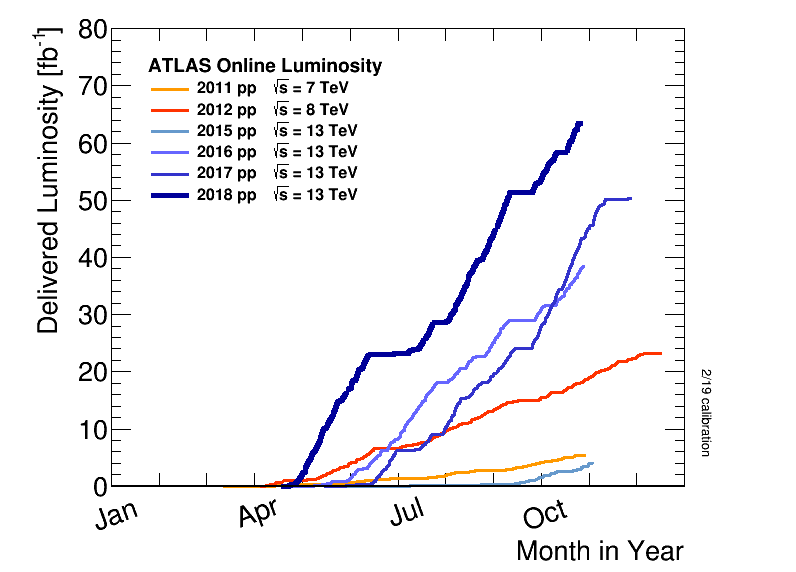
\includegraphics[width=\hsize]{figures/Analysis/lumi.png}
  \caption{Integrated luminosity for data collected from ATLAS from 2011 - 2018}. 
  \label{fig:int_lumi}
\end{figure} 
\FloatBarrier

\begin{figure}[h!]
  \centering
  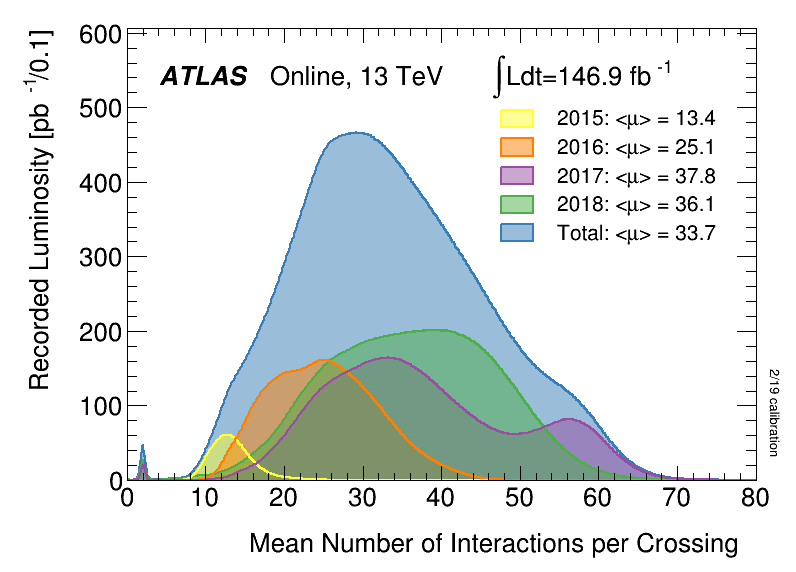
\includegraphics[width=\hsize]{figures/Analysis/mu_profile.png}
  \caption{Mean number of interactions per crossing for data collected from ATLAS from 2011 - 2018}. 
  \label{fig:mu_profile}
\end{figure} 
\FloatBarrier


\section{Simulated Samples}
Samples are simulated in order to model backgrounds, evaluate signal acceptance, optimize event selection and estimate systematic and statistical uncertainties. The dominant backgrounds for this analysis are $W/Z$ + jets, diboson ($WZ$/$WW$), $t\bar{t}$, single top and multijet production. 

$W/Z$+jet events are simulated using Sherpa 2.2.1 at NLO [cite [29]] and merged with the Sherpa parton shower using the ME+PS@NLO prescription \cite{me_ps}. These events are then normalized to NNLO cross sections. The $t\bar{t}$ and single-top backgrounds are generated with Powheg-Box with NNPDF3.0NLO PDF sets in the matrix element calculation [cite[35]]. For all processes, the parton shower, fragmentation, and underlying event are simulated using Pythia 8.320 with the A14 tune set[cite[ATL-PHYS-PUB-2014-02]]. Diboson processes are generated using Sherpa 2.2.1. 

Signal samples are simulated using MadGraph 5-2.2.2 [cite 42] and Pythia 8.186 with NNPDF230LO. RS Graviton samples are generated with $k/M_{PL}$=1. HVT Model A (B) samples are simulated with $g_{V}=1(3)$, as the difference in the width of the samples is smaller than detector resolution. Model C is generated by setting $g_{H}=1$ and $g_{f}=0$ to model VBF production of HVT bosons. Signals are generated for masses between 300 GeV and 5 TeV.

\section{Object Selection} 
\subsection{Electrons}
Electrons are reconstructed from electromagnetic showers in the LAr EM calorimeter. During reconstruction cells of $\Delta \eta \times \Delta \phi = 0.025 \times 0.025 $ are grouped into 3$\times$5 clusters. These clusters are then scanned for local maxima that seed electron clusters. These clusters must then be matched to ID track from the PV. This requirement minimizes non-prompt electron and fake electron backgrounds. Electrons must pass identification and isolation requirements. Electron identification (loose, medium, tight) classification is based on a multivariate discriminant that identifies electrons using a likelihood based method. For this analysis tight electrons are used. Electrons are also required to be isolated. The electrons are considered isolated if the quotient of the sum of the transverse momentum (of calorimeter energy deposits) in a cone around the electron of size $\Delta R = 0.2$ and the transverse momentum of the electron to be less than $0.015*p_{T}$ or 3.5 GeV, whichever is smaller. This requirement rejects non-prompt photons and other fake leptons. Electrons in this analysis are also required to have $p_{T} > 30$ GeV and $|\eta| < 2.47$. Electrons are also required to have $p_{T} > 30$ GeV.

Electrons are calibrated to determine data-driven scale factors using $J/ \Psi \rightarrow ee$, $Z \rightarrow ee$, $Z \rightarrow \ell \ell \gamma$ processes. These corrections account for the  non-uniform response of the detector which introduces modeling and reconstruction uncertainties. 

\subsection{Muons}
As muons traverse the entire detector, they are reconstructed from ID and MS tracks. For this analysis the muon identification and isolation working points are chosen to minimize the contributions from non-prompt muons. Towards this end, the medium muon identification working point is used. For this working point, two types of reconstructed muons are used: combined and extrapolated muons (CB and ME, respectively). For CB muons, ID and MS tracks are reconstructed independently and a combined track fit is performed by adding or removing MS tracks to improve the fit quality. ME muons are reconstructed from only MS tracks with hits in at least two layers, which ensures the track originates from the PV. ME muons extend the acceptance for muon reconstruction outside the ID from $2.5 < |\eta| < 2.7$.
The medium identification working point uses CB and ME tracks. CB tracks must have at least 3 hits in two MDT layers. ME tracks are required to have at least three MDT/CSC hits. To further minimize contributions from fake muons, the selected muons are required to be isolated from other tracks, as muons from $W,Z$ decays are often isolated from other particles. To insure the selected muons are isolated, the scalar sum of the transverse momentum of tracks in a cone of $\Delta R = 0.3$ compared to the transverse momentum of the muon must be less then 0.06. Muons are also required to have $p_{T} > 30$ GeV.

Muons are calibrated using well-studied resonances $J/ \Psi \rightarrow \mu \mu$ (low-$p_T$),  $Z \rightarrow \mu \mu$ (high-$p_{T}$). Figure \ref{fig:muon_syst} shows the combined muon $p_{T}$ uncertainty from this calibration. The total systematic uncertainty is less then 1\% for all $p_{T}$ ranges considered in this analysis.


\begin{figure}[h!]
  \centering
  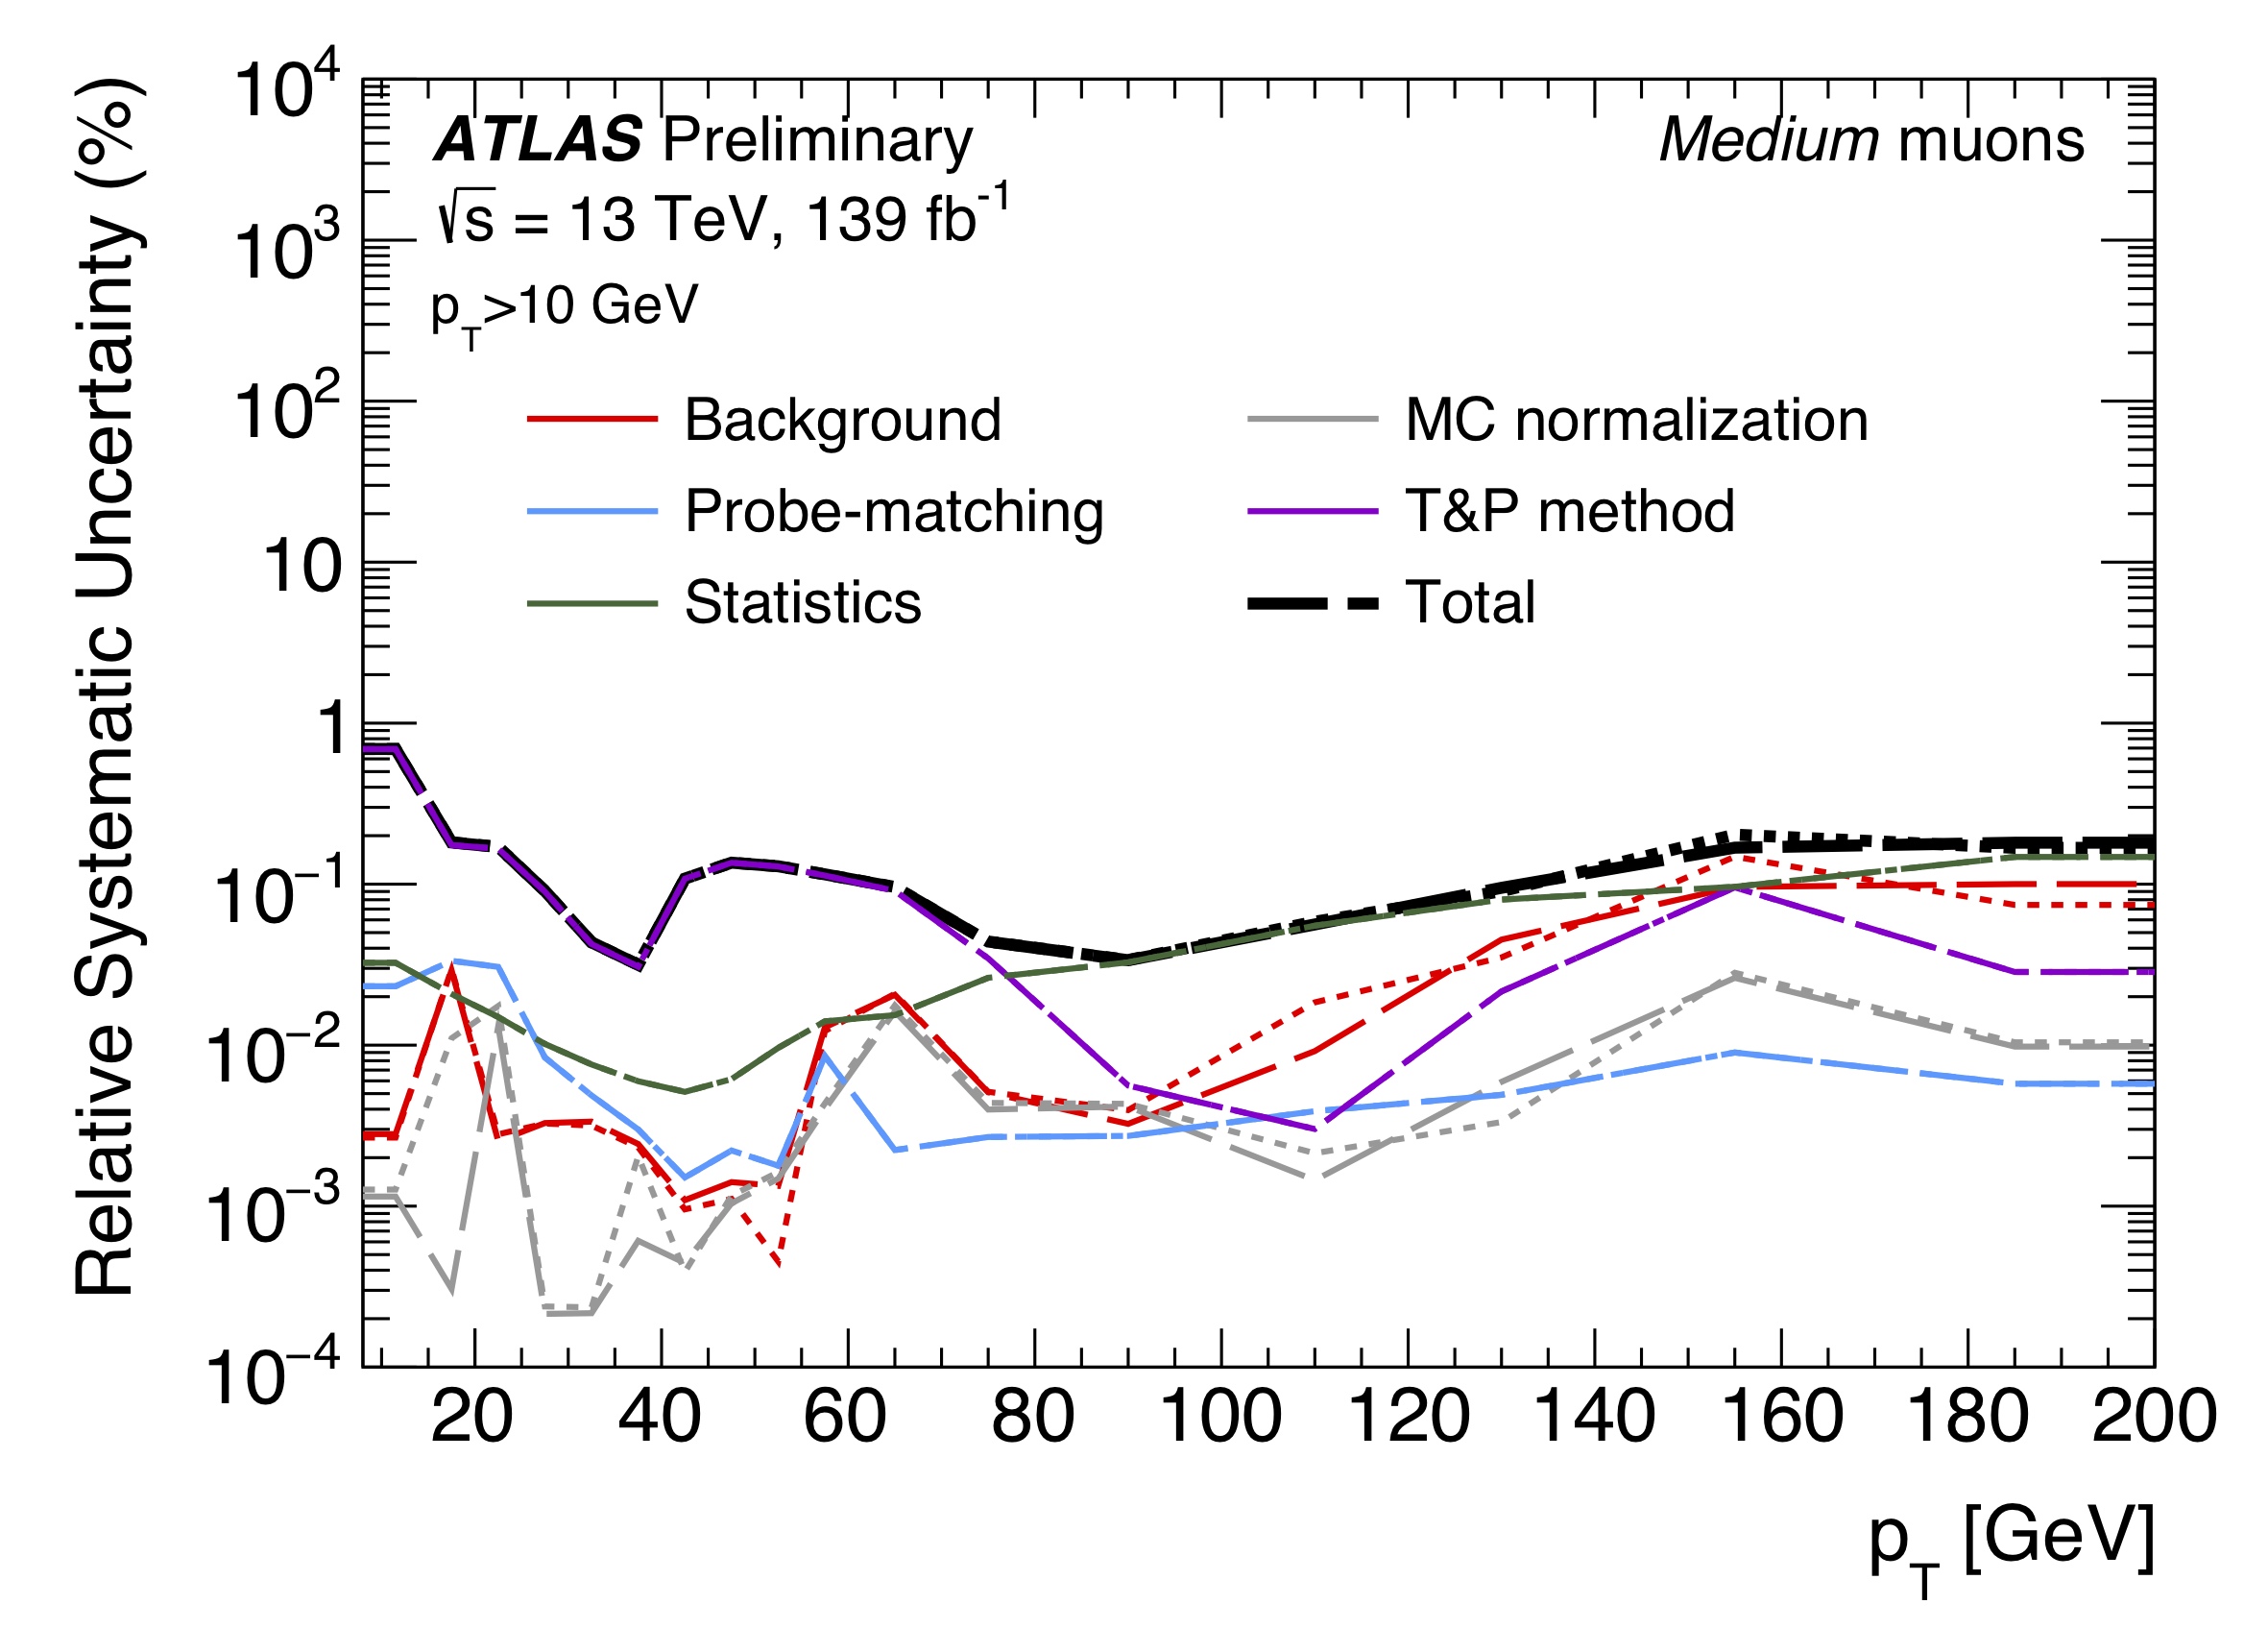
\includegraphics[width=\hsize]{figures/Analysis/muon_syst.png}
  \caption{{This figure shows the breakdown of the muon reconstruction efficiency scale factor measured in $Z \rightarrow \mu \mu$ as a function of $p_{T}$ \cite{muon_calib}. }}. 
  \label{fig:muon_syst}
\end{figure} 
\FloatBarrier

\subsection{small-R jets}
Small-R jets are used to reconstruct the hadronically decaying $W/Z$ candidates in the resolved analysis and VBF jets. These jets are less boosted and therefore spatially separated and reconstructed separately. These jets are constructed from topologically connected clusters of calorimeter cells (topoclusters), seeded from calorimeter cells with energy deposits significantly above the noise threshold.  These cells are then used as inputs to the $anti-k_{t}$ algorithm \cite{antikt} with a distance = 0.4, here called small-R jets. These jets are calibrated to compensate and account for biases from jet reconstruction. 

The jet energy is calibrated sequentially as shown in Figure \ref{fig:jetcalib}. After the jet direction is corrected to point to the PV, the energy of the jet is corrected. First, the jet energy is corrected to account for pileup contributions based on the $p_{T}$ and area of the jet (these corrections are extracted from a $pp \rightarrow jj$ sample). Following this, another pileup correction is applied that scales with $\mu$ and $N_{PV}$. 

MC-based corrections are then applied that are meant to transform the jet energy and $\eta$ back to truth level. Therefore, these corrections account for the non-compensating nature of the ATLAS calorimeters and inhomogeneity of the detector. Following this, the Global Sequential Calibration is applied that reduces flavor dependence of jet calibrations and accounts for energy leakage of jets outside the calorimeters. Finally, in-situ corrections are applied that account for differences in jet responses between data and simulation ($\gamma /Z+$jet and multijet samples are used). These differences can be due to mismodelling of the hard scatter event, pile-up, jet formation, etc. 

Jets used in this analysis must have $p_{T} > 30$ GeV and $|\eta| < 2.5$. To further reduce fake jets the jet-vertex-tagger (JVT) is used to reject pile-up jets [cite 43 P]. The JVT  uses two track-based variables, corrJVF and $R_{p_{T}}$ to calculate the likelihood that the jet originated from the PV. The corrJVF compares the scalar sum of the $p_{T}$ of tracks associated with the jet and PV to the scalar sum of the $p_{T}$ of tracks associated with the jet. This variable also includes a correction that reduces the dependency of corrJVF with the number of reconstructed vertices in the event. The other discriminant, $R_{p_{T}}$, is given by the ratio of the scalar sum of the $p_{T}$ of tracks associated with the jet and PV to the $p_{T}$ of the jet. Both of these variables peak around zero for pileup jets, as these jets are unlikely to have tracks associated with the PV. JVT cuts are applied to all jets with $p_{T} > 120$ GeV. Central jets ($|\eta| < 2.4$) are required to have a JVT > 0.59 and forward jets ($2.4<|\eta| < 2.5$) are required to have JVT > 0.11. 

To further reject fake jets, jets must pass quality requirements based on the following variables ([cite P42]):

\begin{itemize}
\item[-] $f_{Q}^{LAr}$: fraction of energy of jet's LAr cells with poor signal shape
\item[-] $f_{Q}^{HEC}$: fraction of energy of jet's HEC cells with poor signal shape
\item[-] $E_{neg}$: sum of cells with negative energy
\item[-] $f_{EM}$: fraction of jet's energy deposited in EM calorimeter
\item[-] $f_{HEC}$: fraction of jet's energy deposited in HEC calorimeter
\item[-] $f_{max}$: maximum energy fraction in any single calorimeter layer
\item[-] $f_{ch}$: ratio of the scalar sum of the $p_{T}$ of a jet's charged tracks to the jet's $p_{T}$
\end{itemize}

Jets selected for the resolved analysis must pass one of the following criteria:

\begin{itemize}
\item[-] $f_{HEC} > 0.5$ and $|f_{Q}^{HEC}| > 0.5$ and $\left\langle Q \right\rangle $ > 0.8
\item[-] $|E_{neg}| > 60$ GeV
\item[-] $f_{EM} > 0.95$ and $f_{Q}^{LAr} > 0.8$ and $\left\langle Q \right\rangle $ > 0.8 and $|\eta| < 2.8$
\item[-] $f_{max} > 0.99$ and $|\eta| < 2$
\item[-] $f_{EM} < 0.05$ and $f_{ch} < 0.05$ and $|\eta| < 2$
\item[-] $f_{EM} < 0.05$ and  $|\eta| > 2$
\end{itemize}



\begin{figure}[h!]
  \centering
  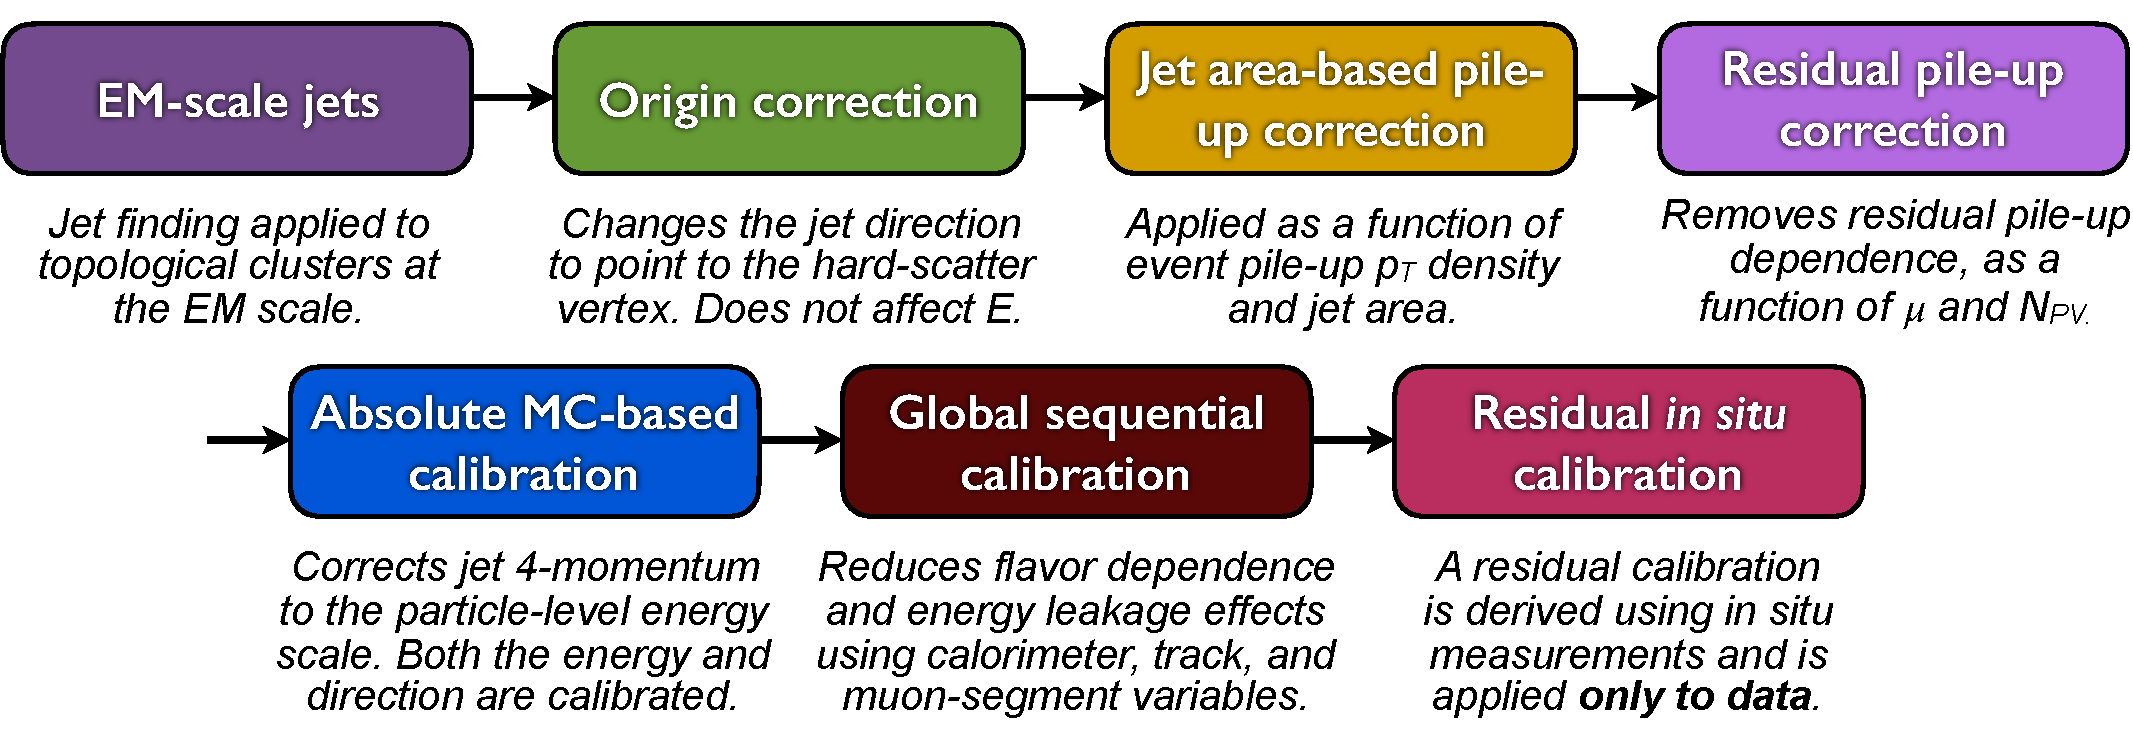
\includegraphics[width=\hsize]{figures/Analysis/jetcalib.pdf}
  \caption{\cite{jetcalib} This diagram shows the calibration stages for EM jets.} 
  \label{fig:jetcalib}
\end{figure} 
\FloatBarrier




\subsection{large-R jets}
Large-R ($\Delta R = 1.0$) jets are used to reconstruct the high-$p_{T}$ $W/Z \rightarrow qq$ candidates in the merged analysis. Track-Calo Clusters (TCCs) are used to reconstruct these jets [cite ANA 50]. These jets are constructed via a pseudo particle flow method using ID tracks matched to calorimeter clusters. The angular resolution of the calorimeter degrades sharply with jet $p_{T}$, but the jet energy resolution improves. The tracker has excellent angular resolution which improves with $p_{T}$. Therefore, by matching tracks to jets, TCCs have more precise energy and angular resolution than jets constructed from calorimeter information only. These jets are required to have $p_{T}>200$ GeV, $|\eta| < 2.0$ and $m_{J} > 50$ GeV. 

TCC jets are trimmed as detailed in [cite ANA 45], which suppresses pileup and soft radiation in the jet, the jet mass is calculated as the four-vector sum of the jet's constituents (assuming massless constituents). The jet mass peaks around the $W/Z$ boson mass for $W/Z \rightarrow qq$ jets, and more broadly for quark and gluon induced jets. 

These jets are then tagged as $W/Z$ jets if they pass the jet mass and $D_{2}$ cuts. The jet substructure variable $D_{2}$ is given by the ratio of energy correlation functions based on energies and pair-wise angles of a jet's constituents [cite ANA 46, 47]:

\begin{equation}
D_{2}^{\beta=1} = E_{CF3}\left(\frac{E_{CF1}}{E_{CF2}}\right)^{3}
\end{equation}

Where the energy correlation functions are defined as:
\begin{equation}
E_{CF1}=\sum_{i}p_{T,i}
\end{equation}
\begin{equation}
E_{CF2}=\sum_{ij}p_{T,i}p_{T,j}\Delta R_{ij}
\end{equation}
\begin{equation}
E_{CF3}=\sum_{ijk}p_{T,i}p_{T,j}p_{T,k}\Delta R_{ij}\Delta R_{jk}\Delta R_{ki}
\end{equation}

A two-dimensional optimization of the jet mass and $D_{2}$ thresholds was performed to provide maximum sensitivity for this analysis. Figure \ref{fig:wztag_eff} shows the optimized thresholds on $D_{2}$ and jet mass as a function of $p_{T}$. Figure \ref{fig:boson_tagger_optimization} shows the efficiency of the optimized $W/Z$ taggers as a function of jet $p_{T}$. 


\begin{figure}[h]
%\subfloat[][\label{fig:D2_W}]{
    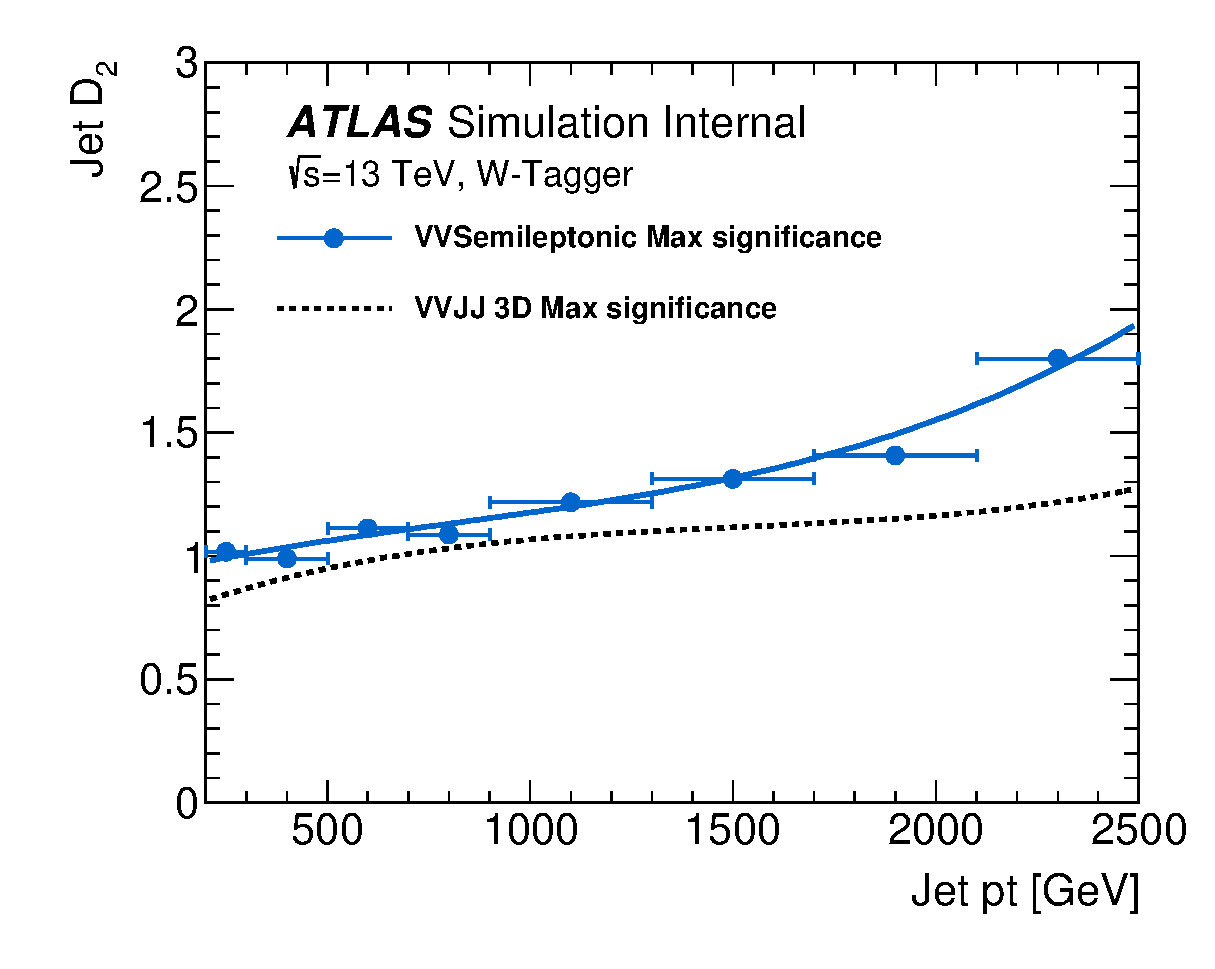
\includegraphics[width=0.48\hsize]{figures/Analysis/D2_W_Fit.eps}
%}
%\subfloat[][\label{fig:Mass_W}]{
    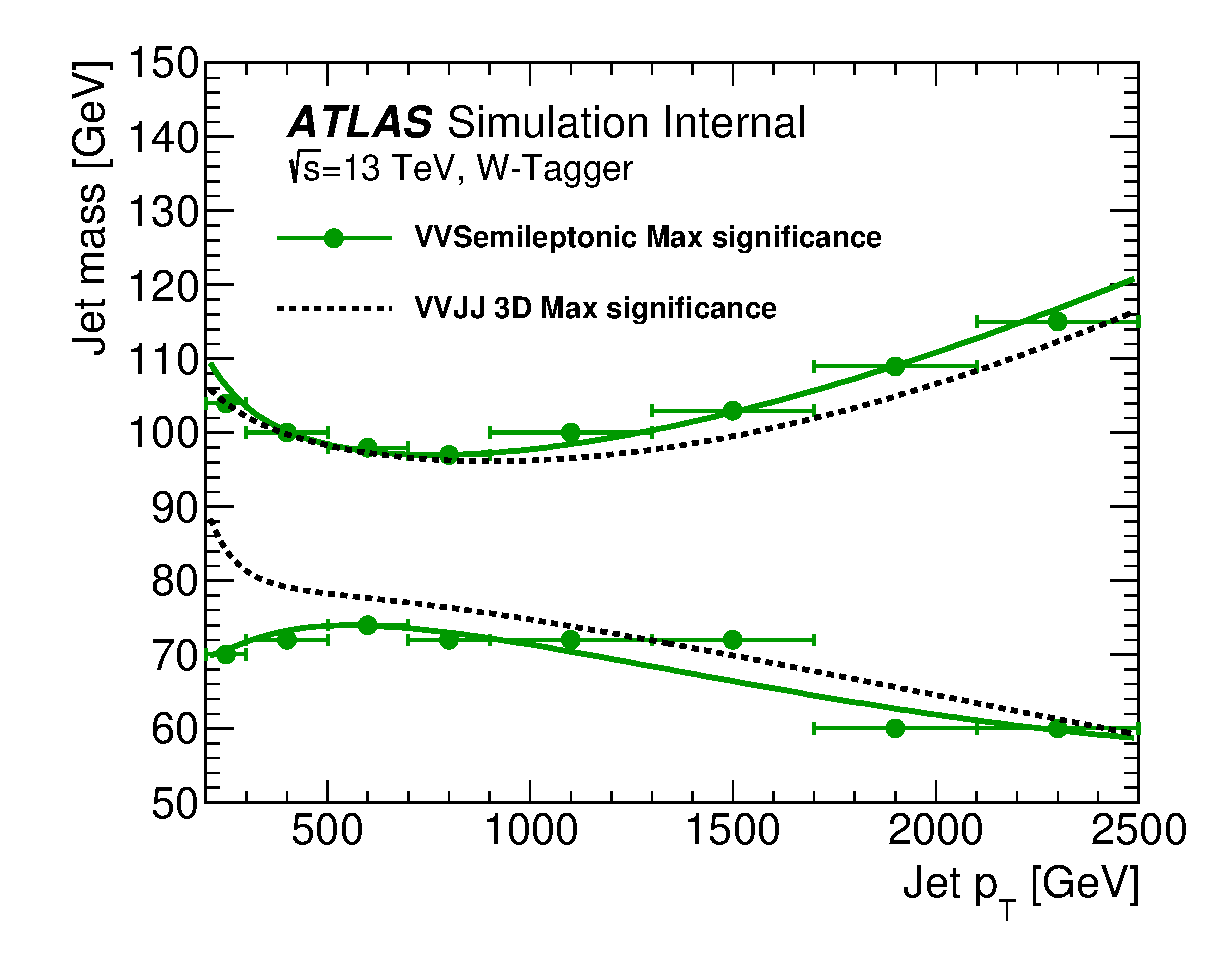
\includegraphics[width=0.48\hsize]{figures/Analysis/Mass_W_Fit.eps}
%}

%\subfloat[][\label{fig:D2_Z}]{
    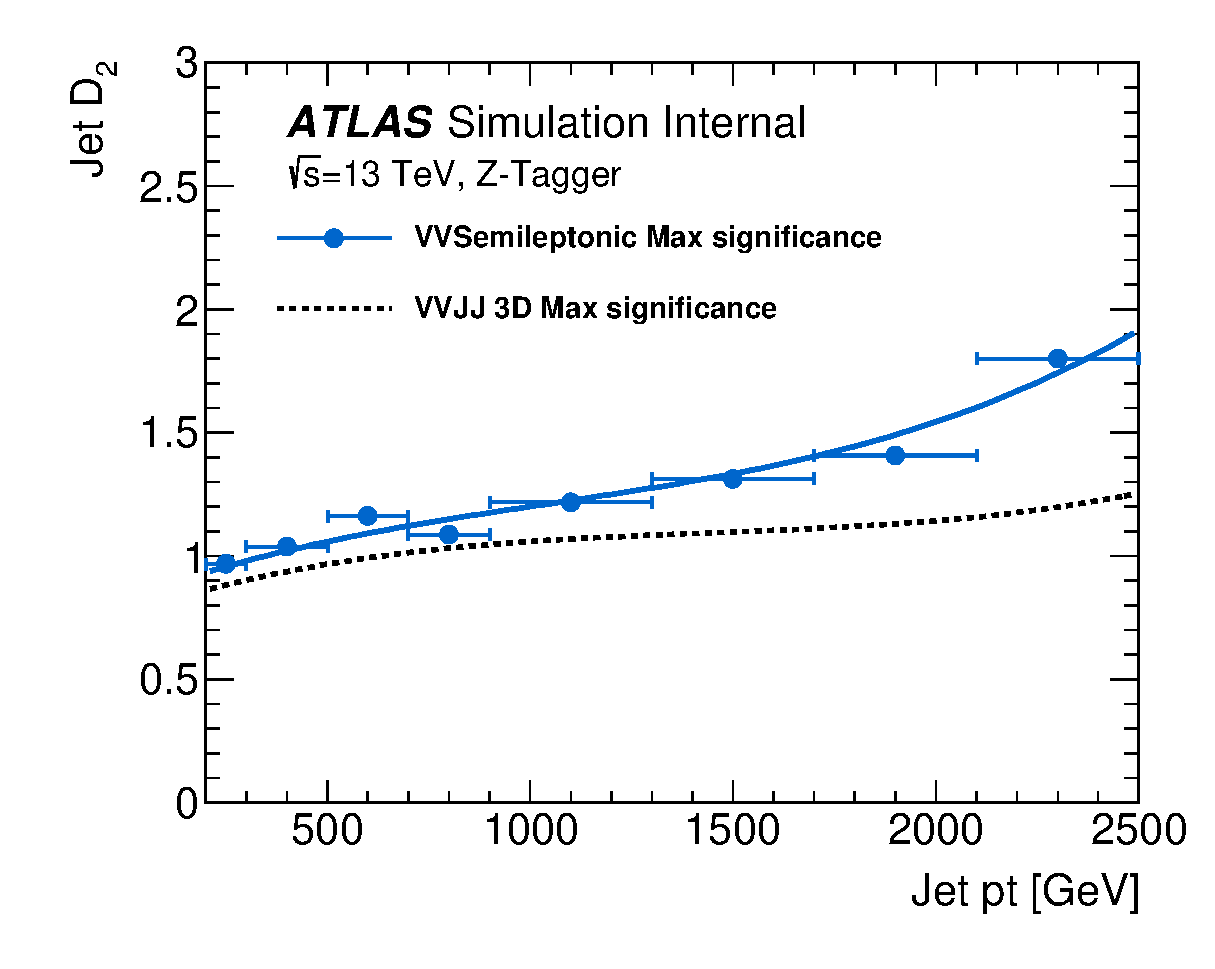
\includegraphics[width=0.48\hsize]{figures/Analysis/D2_Z_Fit.eps}
%}
%\subfloat[][\label{fig:Mass_Z}]{
    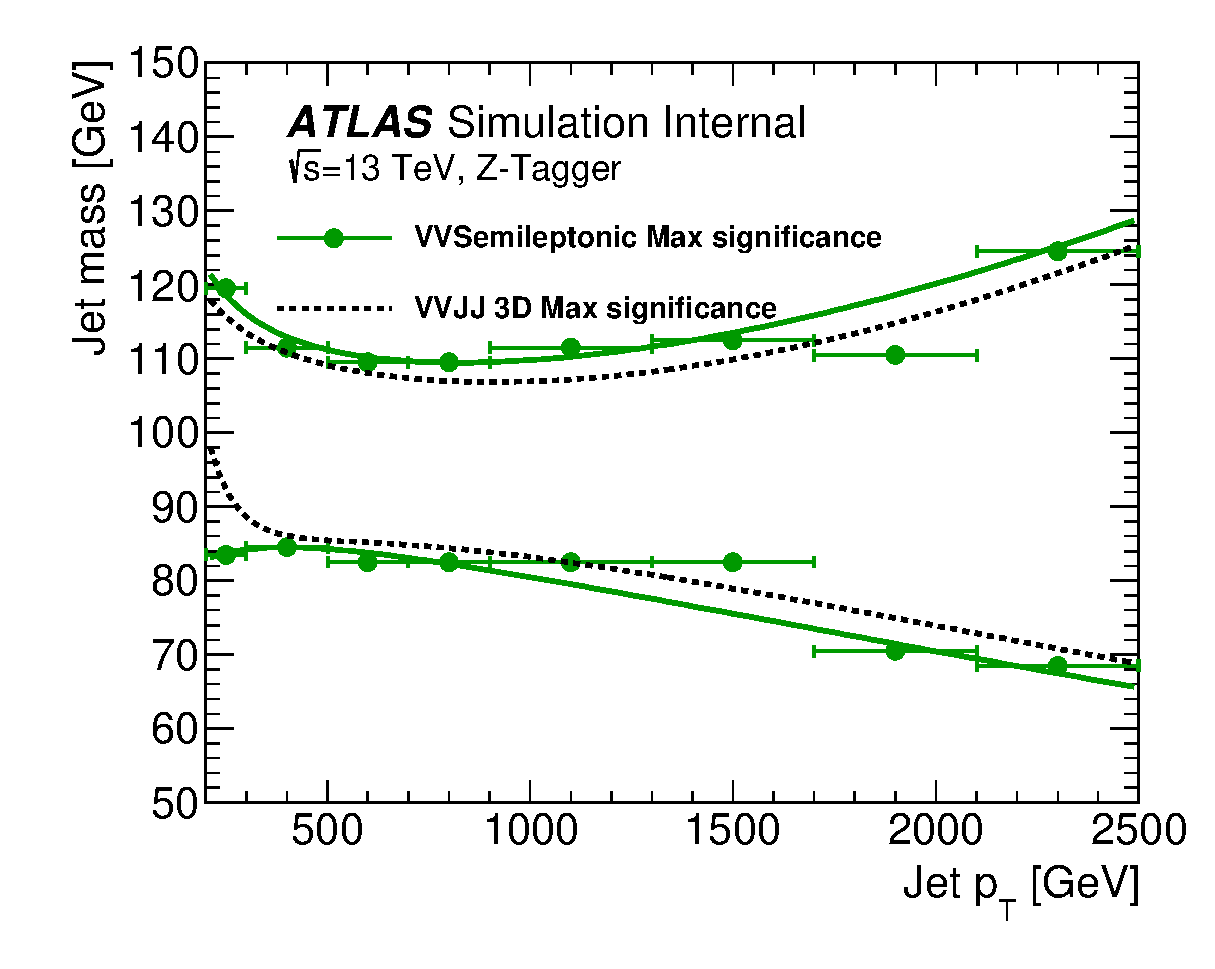
\includegraphics[width=0.48\hsize]{figures/Analysis/Mass_Z_Fit.eps}
%}
\caption{The upper cut on $D_2$ (a) and jet mass window cut i.e. the upper and lower boundary of the mass (b) of the $W$-tagger as a function of jet $p_{T}$. Corresponding values for $Z$-tagger are shown in (c) and (d). The optimal cut values for maximum significance are shown as solid markers and the fitted function as solid lines. Working points from $VV\to JJ$[ATLAS-HDBS-2018-31-002] is also shown as dashed lines as a reference. Natasha reword?}
\label{fig:wztag_eff}
\end{figure}
\FloatBarrier



\begin{figure}[h!]
  \centering
  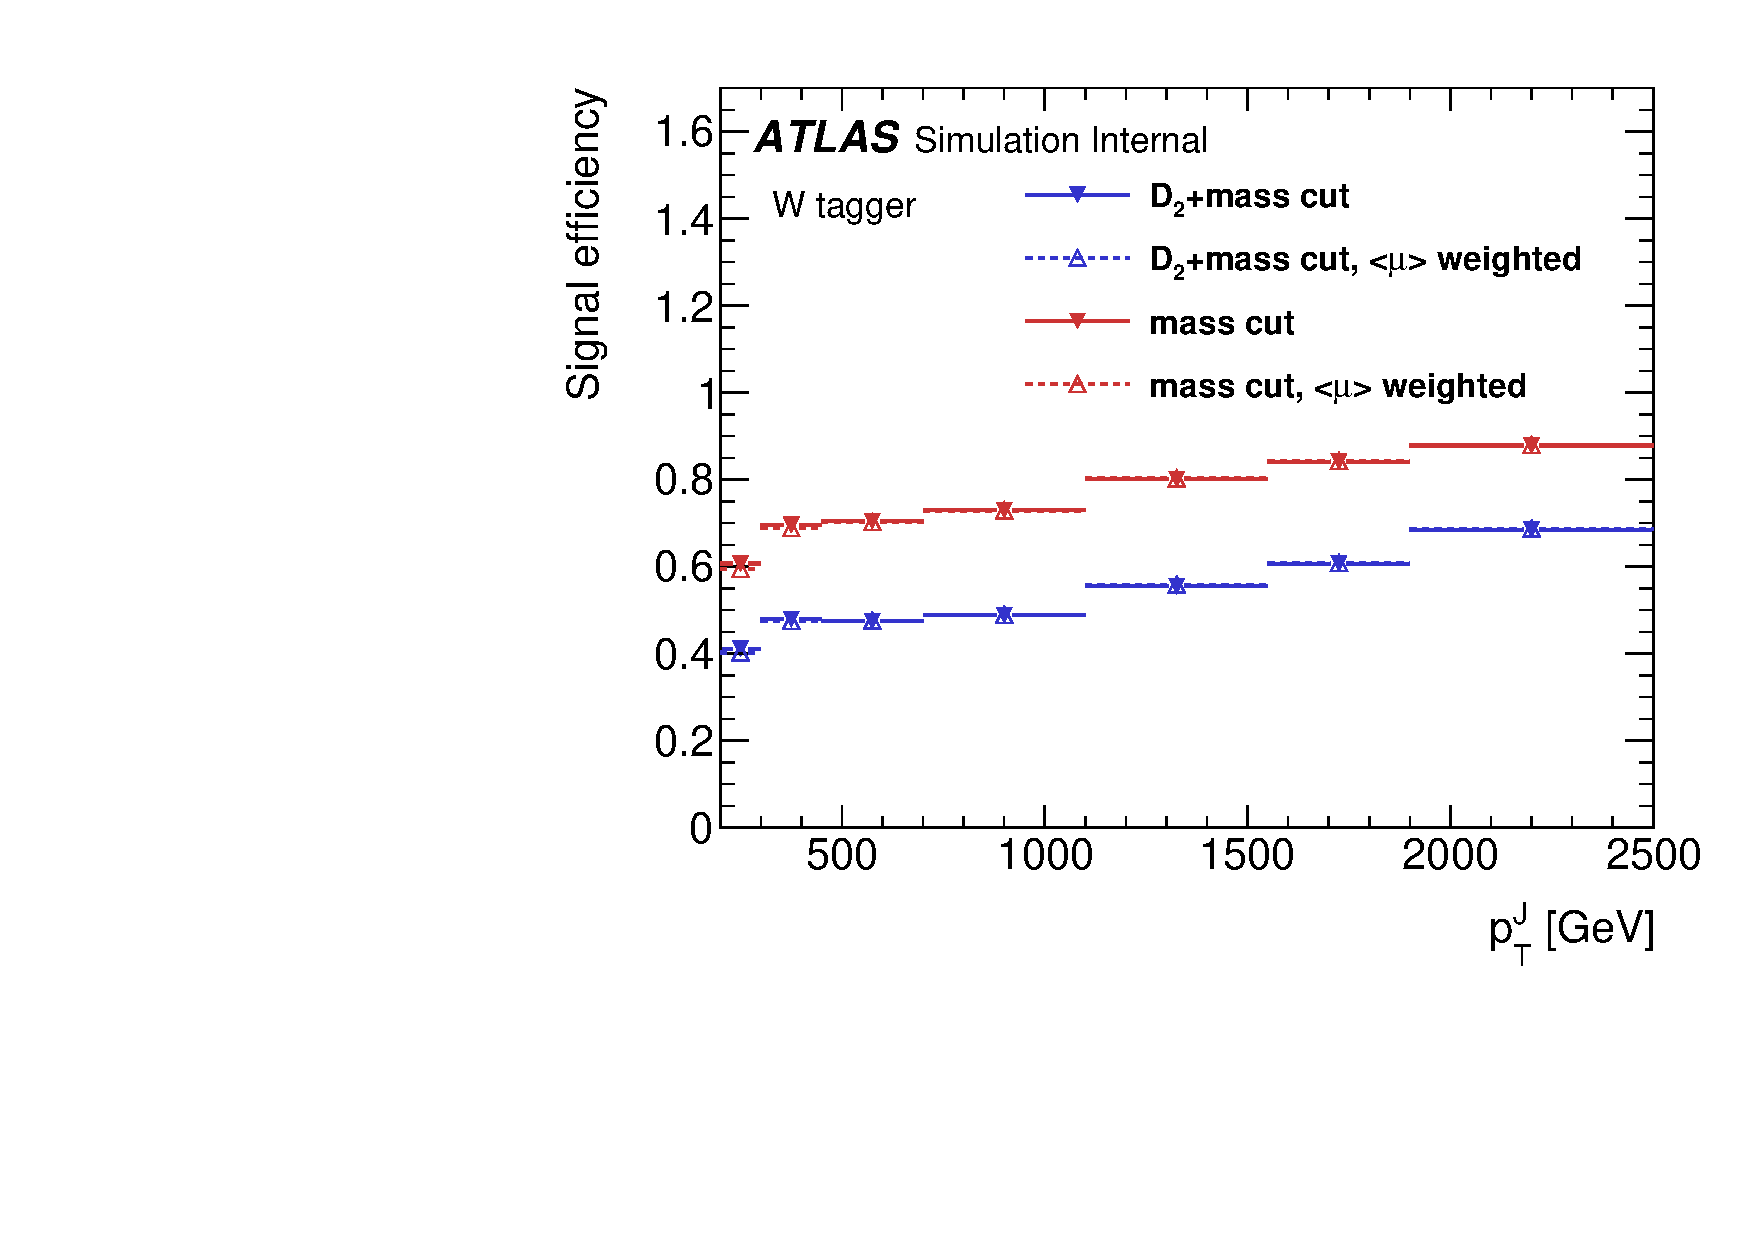
\includegraphics[width=0.48\hsize]{figures/Analysis/sigeffW.pdf}
  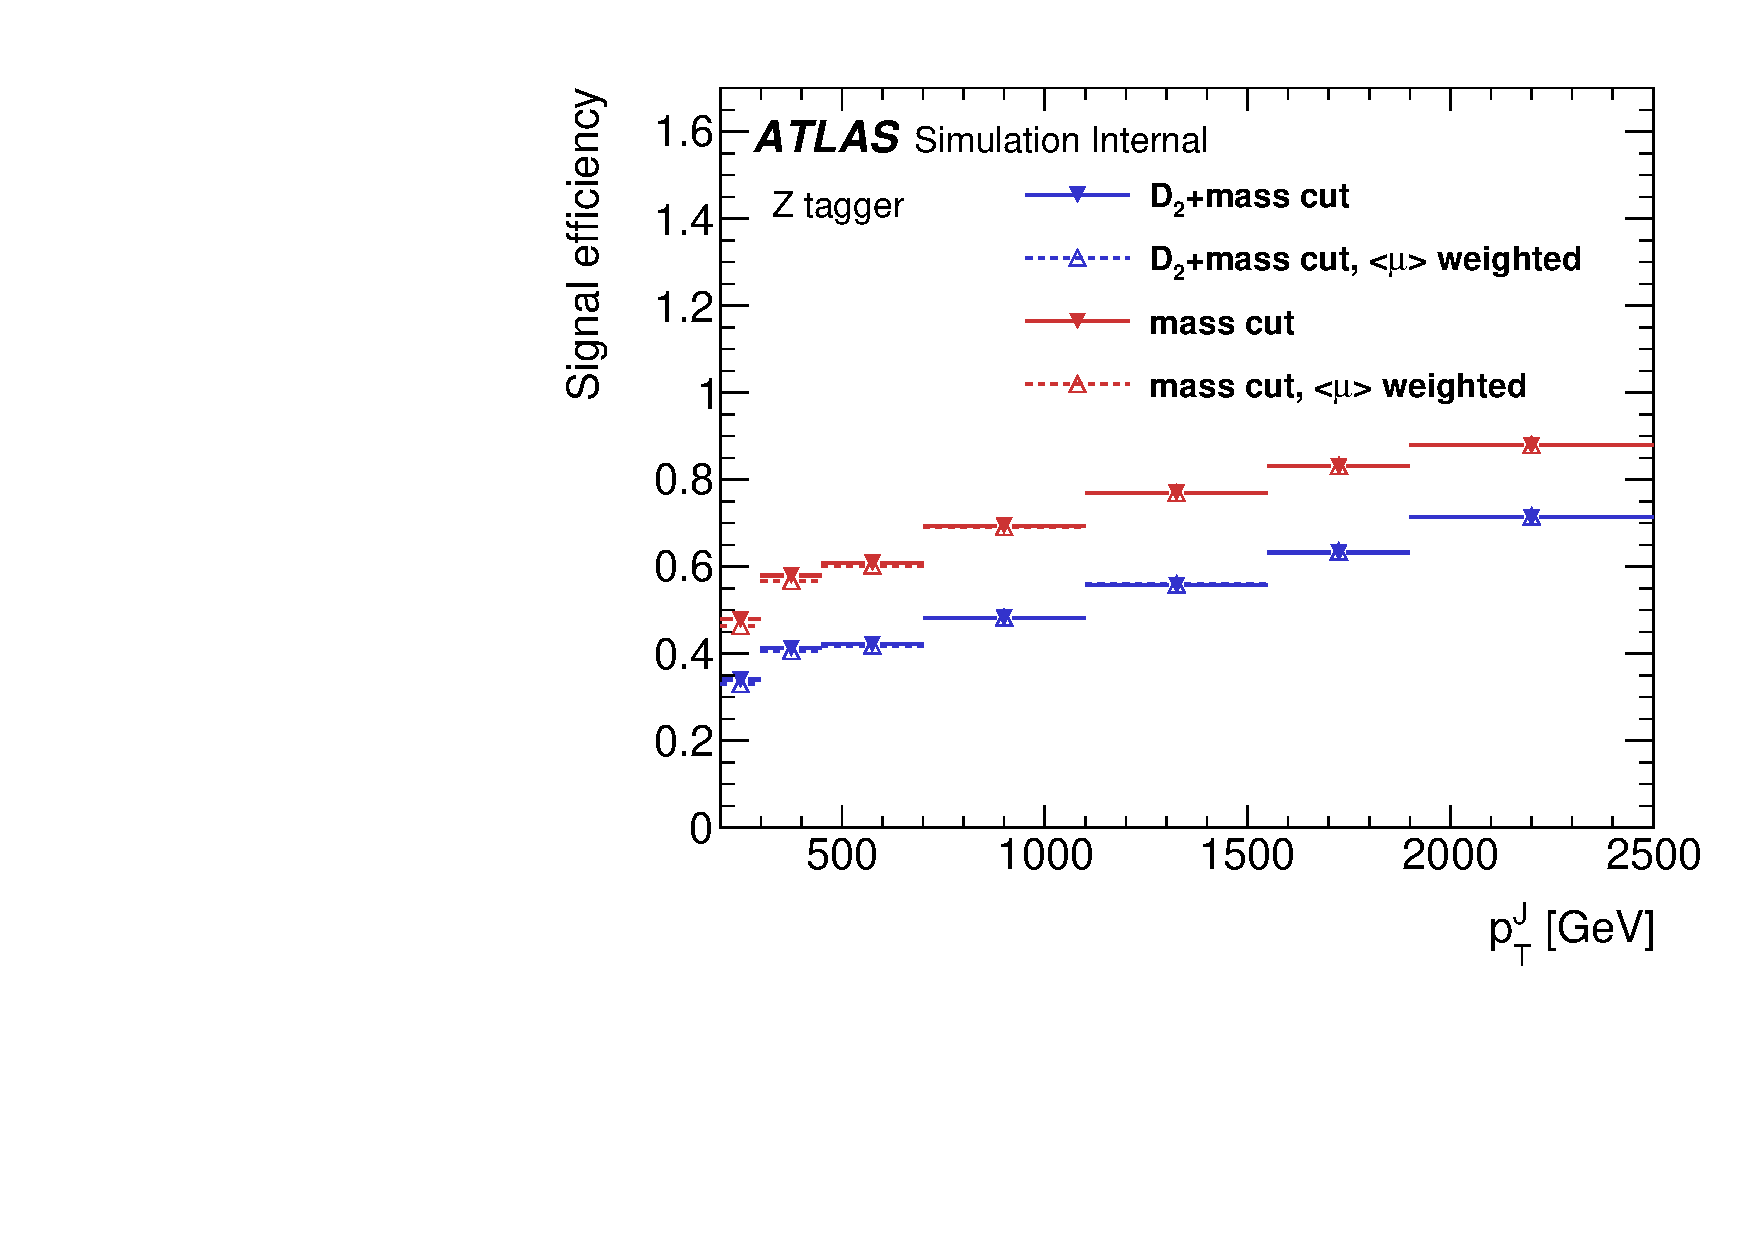
\includegraphics[width=0.48\hsize]{figures/Analysis/sigeffZ.pdf}
  \caption{Natasha write caption} 
  \label{fig:boson_tagger_optimization}
\end{figure} 
\FloatBarrier




\subsection{Variable Radius jets}
Variable-radius (VR) track jets are used to identify b-quark induced jets within the catchment area of large-R jets [cite ANA 52]. These jets use a $p_{T}$ dependent cone size defined as: 
\begin{equation}
R_{eff}(p_{T, i}) = \frac{\rho}{p_{T,i}}
\end{equation}
for building jets from ID tracks with an anti-$k_{t}$ algorithm. For this analysis $\rho=30$ GeV and an upper and lower limit on cone size are set to 0.02 and 0.4, respectively. Collinear VR jets are possible, so track jets that are not separated by the the smaller jet's cone size are not used. These jets are also required to have $p_{T} > $ 10 GeV and $|\eta| < 2.5$. 


\subsection{MET/neutrinos}
As neutrinos are uncharged and colorless they do not leave tracks or jets in the detector. For this reason, neutrinos are reconstructed calculated the $E_{T}^{miss}$, the negative vector sum of $p_{T}$ all the physics objects and an extra "soft" term. The "soft" term accounts for energy deposits not associated with any of the objects in the event. For this analysis the soft term is given by the sum $p_{T}$ of all ID tracks not associated with objects in the event. The selected tracks must be matched to the primary vertex, which decreases pile-up contamination [cite G 217 218]. The tight working point is used [Natasha look up what this means].  

\subsection{Jet Flavor Tagging}
To further classify events, the small radius jets originating from a b-quark are classified using a multivariate $b$-tagging algorithm (BDT), MV2c10 [cite G 210 199]. This algorithm uses the impact parameters of the jet's ID tracks, secondary vertices (if they exist), and reconstructed flight paths of $b$ and $c$ hadrons in the jet to determine if the jet was induced by a $b$-quark. For this analysis the 85\% efficient working point of this algorithm is used giving $c$, $\tau$, and light-flavor jet rejection of 3, 8, and 34 respectively in a simulated $t\bar{t}$.


\subsection{Overlap Removal}
Reconstructed jets and leptons in this analysis can arise from the same energy deposits. For instance, a cluster of energy from an electron can also be a valid calorimeter seed for a jet. To mitigate this confusion of multiple objects originating from a single jet or lepton overlapping objects are removed via a procedure referred to a overlap removal. In this procedure the separation of the two objects, $\Delta (R) = \sqrt{(\Delta \eta)^{2}+(\Delta \phi)^{2}}$ determines which object is removed from the event. 

The overlap selections used in this analysis are:

\begin{itemize}
\item[-] when an electron shares a track with another electron with the lower $p_{T}$ electron is rejected, as it is more likely to be a fake electron
\item[-] when a muon and electron share a track the muon is rejected if it is a calo-muon, otherwise the electron is rejected
\item[-] when $\Delta R < 0.2$ for an electron and jet, the jet is rejected to maximize signal acceptance
\item[-] when $\Delta R > 0.2$ for an electron and jet, the electron is rejected as likely originated from decays within the jet
\item[-] when $\Delta R <$min$(0.4, 0.04+10$GeV/$p_{T}^{\mu})$ the muon is rejected, again maximizing signal acceptance, otherwise the jet is rejected
\item[-] when $\Delta R < 1.0$ for the a large-R jet and electron, the jet is rejected

\end{itemize}

\chapter{Event Selection and Categorization}

\section{Pre-selection}
Before applying topological cuts to suppress backgrounds and reduce data size in this search, preselection cuts are applied which include trigger and event requirements. Events must contain exactly one tight lepton (no additional loose leptons),  the $p_{T}^{\ell \nu} > 75$ GeV, and there must be at least two small-R jets or one large-R jet.
\section{Trigger}
The data were collected using the lowest unprescaled single-lepton or $E_{T}^{miss}$ triggers, as summarized in Table \ref{tbl:triggers}. Since the muon term is not considered in the trigger $E_{T}^{miss}$ calculation, the $E_{T}^{miss}$ trigger is fully efficient to events with high-$p_{T}$ muons. For this reason, the $E_{T}^{miss}$  trigger is used for events where $p_{T}^{\mu} > 150$ GeV, to compensate for the poor efficiency of the single muon trigger above $p_{T}^{\mu}>150$GeV. 


\begin{landscape}
\begin{table}[p]
  \caption{The list of triggers used in the analysis.} \label{tab:triggers}
\begin{center} 
\small
\begin{tabular}{|l|c|c|c|}
\hline
Data-taking period & $e\nu qq$ channel & $\mu\nu qq$ ($p_{T}(\mu\nu)<150$ GeV) channel & $\mu\nu qq$ ($p_{T}(\mu\nu) > 150$ GeV) channel  \\
\hline
\hline
\multirow{3}{*}{\centering {2015}} & HLT\_e24\_lhmedium\_L1EM20 OR & HLT\_mu20\_iloose\_L1MU15 OR & \multirow{3}{*}{ HLT\_xe70 } \\
 & HLT\_e60\_lhmedium OR & HLT\_mu50 & \\
 & HLT\_e120\_lhloose & & \\
\hline
\multirow{2}{*}{\centering {2016a (run $< 302919$)}} & HLT\_e26\_lhtight\_nod0\_ivarloose OR & HLT\_mu26\_ivarmedium OR  & \multirow{3}{*}{ HLT\_xe90\_mht\_L1XE50 } \\
 & HLT\_e60\_lhmedium\_nod0 OR & HLT\_mu50 &  \\ 
\multirow{2}{*}{($L<1.0\times10^{34}\,{\textrm cm}^{-2}\,{\textrm s}^{-1}$)} & HLT\_e140\_lhloose\_nod0 & & \\
 & HLT\_e300\_etcut & & \\
\hline
{\centering {2016b (run $\geq 302919$)}} & \multirow{2}{*}{same as above} & \multirow{2}{*}{same as above}  &  \multirow{2}{*}{HLT\_xe110\_mht\_L1XE50} \\
($L<1.7\times10^{34}\,{\textrm cm}^{-2}\,{\textrm s}^{-1}$) & & &\\
\hline
{\centering {2017}} & same as above & same as above  &  HLT\_xe110\_pufit\_L1XE55 \\
\hline
{\centering {2018}} & same as above & same as above  &  HLT\_xe110\_pufit\_xe70\_L1XE50  \\
\hline
\end{tabular}
\end{center}
\end{table}
\end{landscape}
\section{GGF/VBF RNN}
To classify events as originating from GGF/DY or VBF production a recursive neural network (RNN \cite{rnn}) is used. This approach is more powerful than a cut-based classification as it improves signal efficiency and analysis sensitivity by exploiting correlations between variables that the RNN learns. In particular, a RNN architecture is ideal as it can handle variable numbers of jets in the events.  

The RNN uses the four-momentum of candidate VBF jets to classify events as VBF or GGF topologies. As sometimes jets will be incorrectly reconstructed the number of jets in the event are expected to vary across the inputs samples. VBF candidate jets are identified by removing jets from the event that are likely from $W/Z \rightarrow qq$. For the resolved regime this means removing the two leading small-R jets from the VBF candidate jet list. For the merged regime this means removing small-R jets separated by less than 1.0 in $dR$ from the large-R jet. VBF candidate jets are also required to be within $|\eta| < 4.5$. From the list of remaining VBF candidate jets, the two highest-$p_{T}$ jets are chosen. 

The architecture of the RNN is show in Figure \ref{fig:rnn_architecture}. LSTMs are a type of RNN that extract meaningful information and can retain it (unlike other neural networks architectures). This is useful for VBF event classification for events with two jets, where using the kinematic properties of both jets (and their correlations) will lead to more efficient event classification.

In this RNN architecture, the VBF candidates are first passed to a masking layer which checks the number of jets in the event. If there is only one jet, only one LSTM layer is used. The output of masking is then passed to a Long Short-Term Memory (LSTM) cell, with a tanh activation function. This output is passed to a dropout layer, that has a probability of 0.3 to completely forget the output of the LSTM. Dropout is a regularization method, that prevents over-fitting. The output of the dropout layer is then passed to the second LSTM and then through another dropout layer with a probability of 0.3. 

The weights and other parameters of the network are learned by training the network with VBF and GGF signals over 200 epochs with an Adam Optimizer [natasha add reference]. The training is truncated if the network parameters are unchanged after ten iterations. The training, testing and validation sets are 56, 30, and 14 percent of the input samples, respectively. Figure [add INT figure 32] shows the loss function of the network as a function of training epochs. The validation test set has a smaller loss function as dropout was not applied. Figure \ref{fig:rnn_roc} shows the ROC curve for the RNN using k-fold cross validation. 

Finally this output is passed to a dense layer [natasha ask antonio about this] and then to a sigmoid activation layer, leading to an overall RNN score. Figure \ref{fig:rnn_score} shows the RNN discriminant for backgrounds, GGF signals, and VBF signals. The RNN score is $\sim$ 0 for GGF and background processes and $\sim$1 for VBF processes. Figure \ref{fig:rnn_limits} shows the limits for various signal processes based on the RNN cut applied. Requiring the RNN score to be $>$ 0.8 was chosen as it provided the best significance (and signal efficiency) across for this final state and the $\nu\nu qq$ and $\ell \ell qq$ channels this channel will be combined with for future publications.


\begin{figure}[h!]
  \centering
  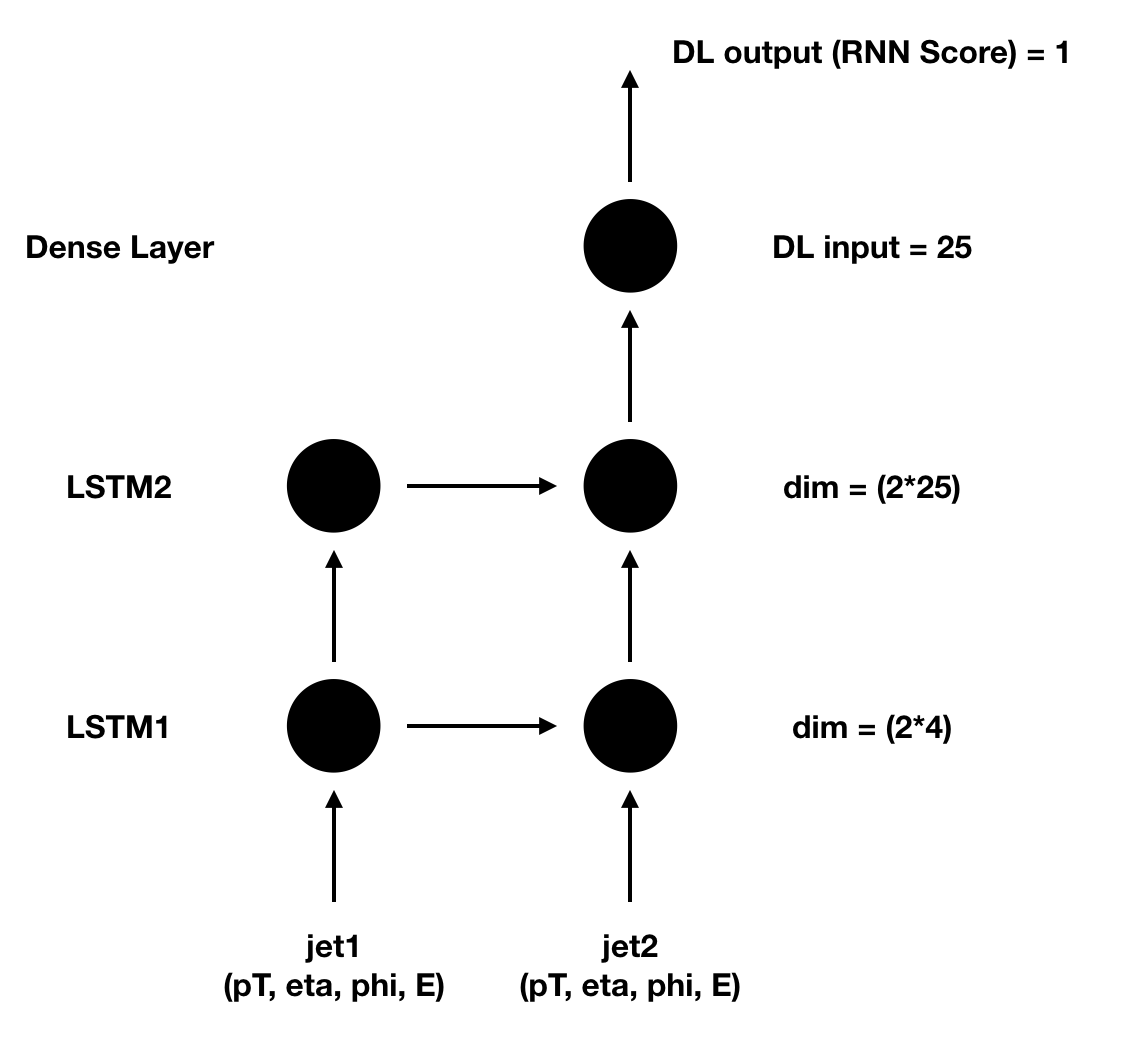
\includegraphics[width=\hsize]{figures/Analysis/rnn_architecture.png}
  \caption{RNN architecture. Natasha add caption} 
  \label{fig:rnn_architecture}
\end{figure}
\FloatBarrier


\begin{figure}[h!]
  \centering
  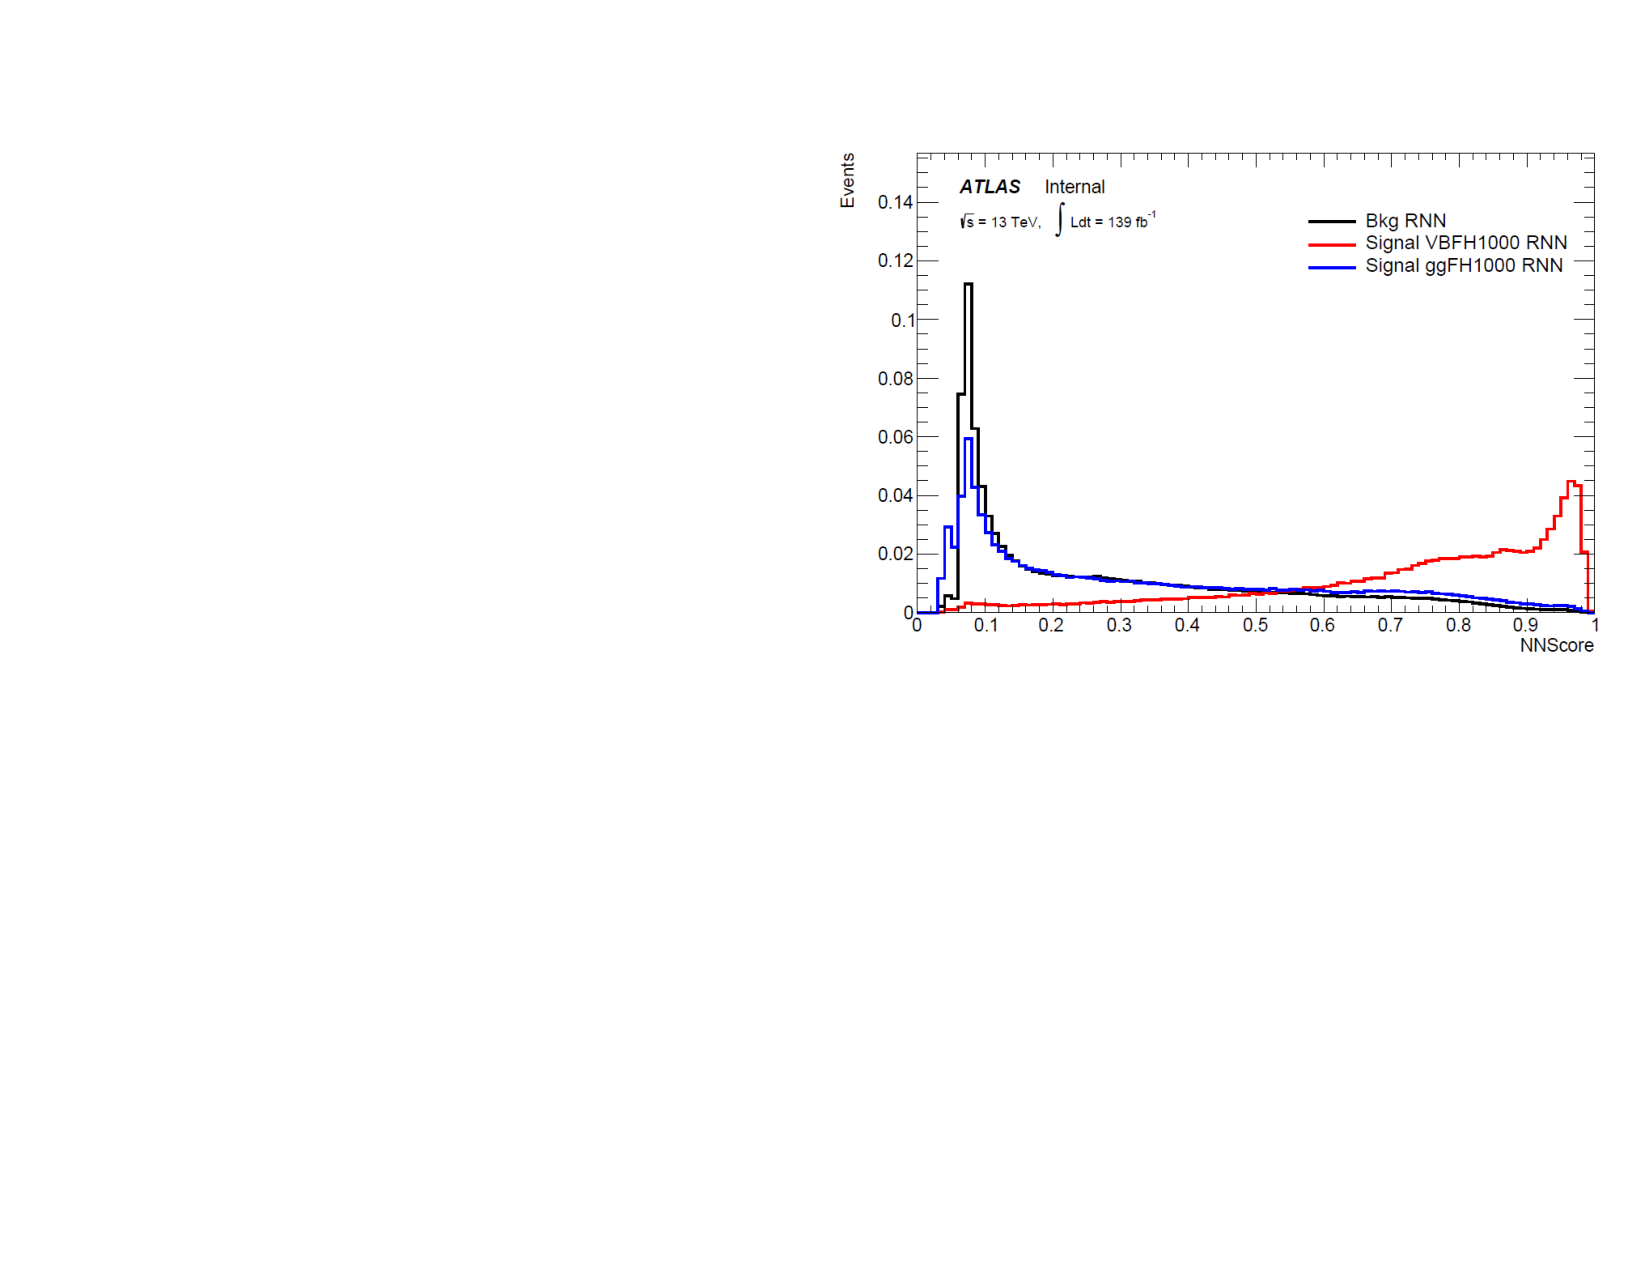
\includegraphics[width=\hsize]{figures/Analysis/rnn.pdf}
  \caption{RNN Score distribution for ggF and VBF signals and backgrounds.} 
  \label{fig:rnn_score}
\end{figure}
\FloatBarrier



\begin{figure}[h!]
  \centering
  \includegraphics[width=\hsize]{figures/Analysis/kFold_ROC.png}
  \caption{ROC curve using k-fold validation for RNN.} 
  \label{fig:rnn_roc}
\end{figure}
\FloatBarrier



\begin{figure}[h!]
  \centering
  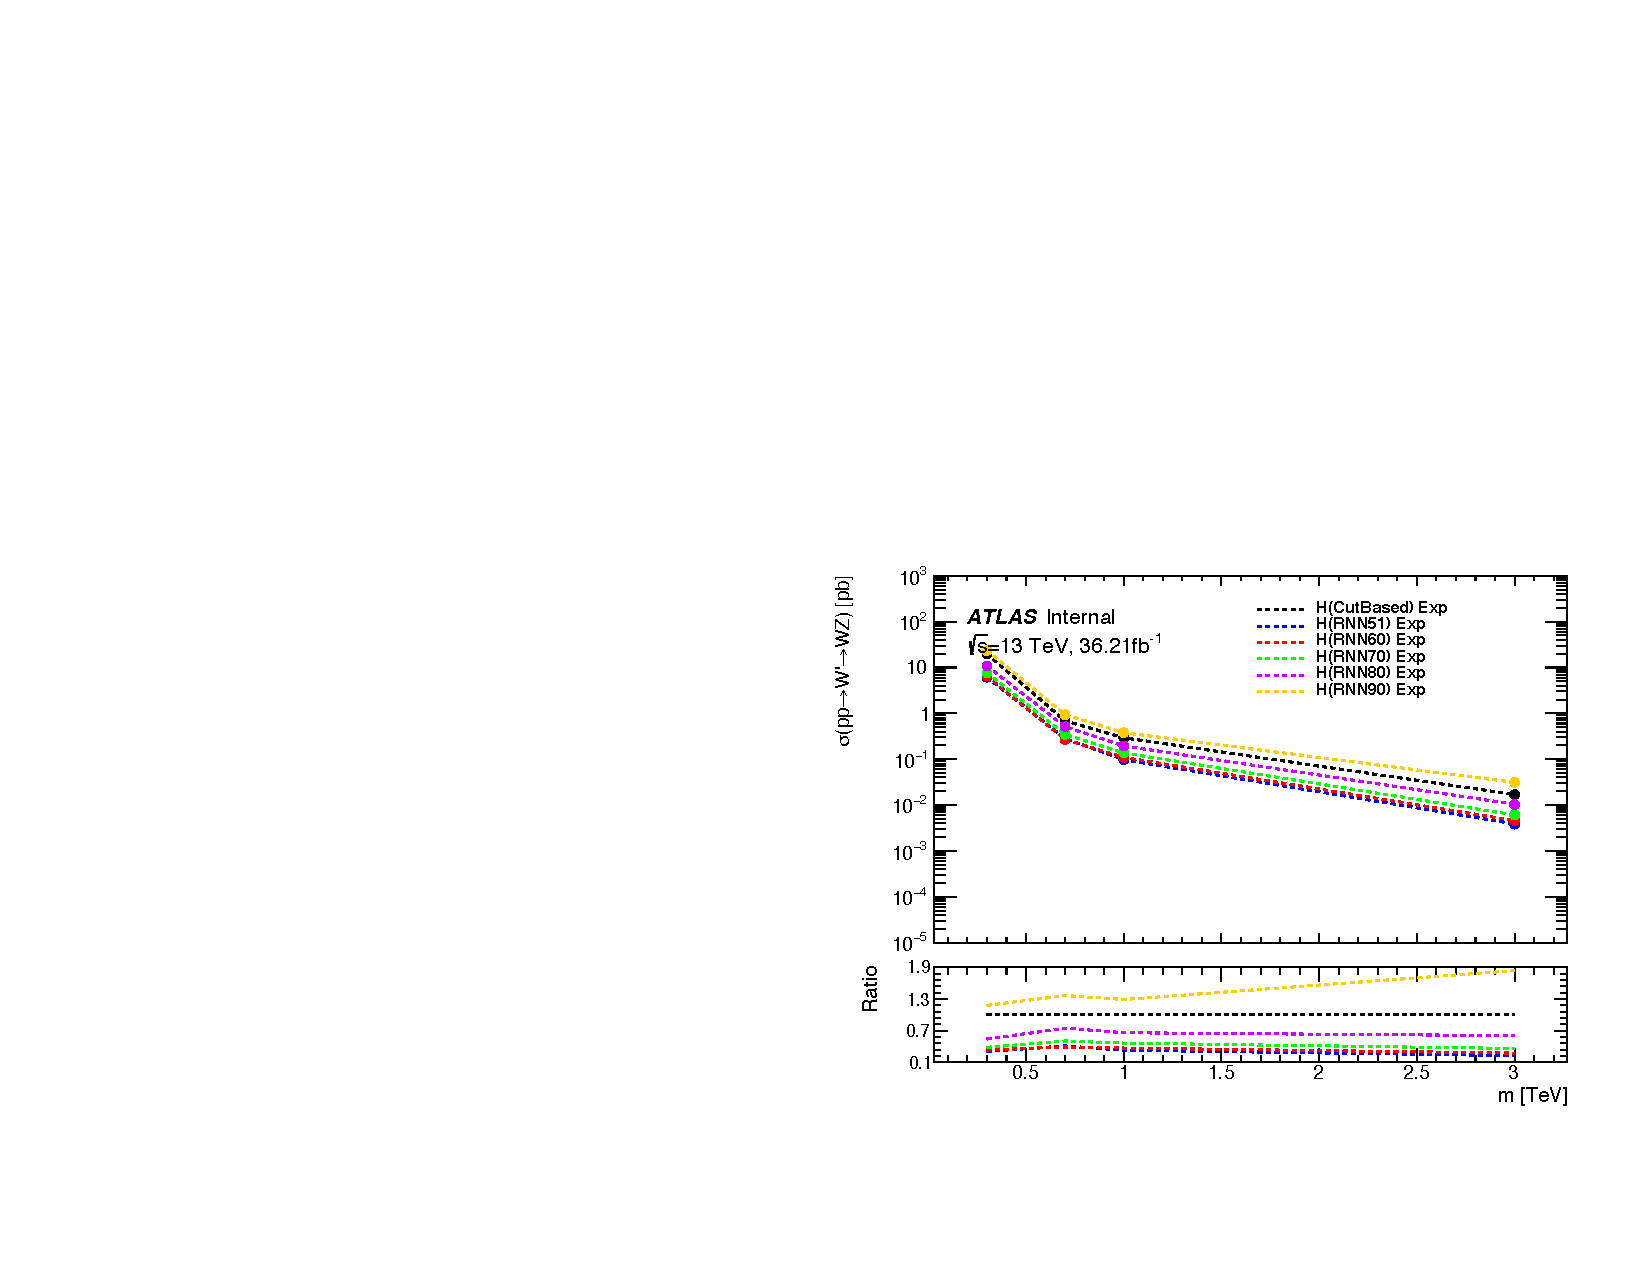
\includegraphics[width=\hsize]{figures/Analysis/rnn_limits.pdf}
  \caption{Comparison of GGF Z' limits for different RNN score selections. The bottom panel shows the ratio of the upper limits set for different RNN cuts to the cut-based analysis. In this panel smaller numbers, indicate that the expected upper limit is smaller than the cut-based analysis, which is desired.} 
  \label{fig:rnn_limits}
\end{figure}
\FloatBarrier

\section{Topological Cuts}
Once an event is classified as VBF or GGF via the RNN, it must pass other topological cuts that maximize $S/\sqrt{B}$. First, to efficiently select events with a $W\rightarrow \ell \nu$ candidate exactly one tight lepton is required and $E_{T}^{miss} > 100(60)$ GeV and $p_{T,\ell\nu} > 200(75)$ GeV in the merged (resolved) analysis to suppress the multi-jet background. 

For the merged analysis, in addition to the $W \rightarrow \ell \nu$ and $W/Z \rightarrow J$ selections above, the min$(p_{T, \ell \nu}, p_{T,J})/m_{WV} > 0.35(0.25)$ for the GGF (VBF) category. To reduce $t\bar{t}$ contamination events with the signal region and $W$+jets control region events with at least one b jet with $\Delta R > 1.0$ from the large-R jet are excluded. High purity signal regions require the $D_{2}$ and $W/Z$ mass window cut to be passed, whereas the low purity region only requires the  $W/Z$ mass window cut to be passed. Finally for events to be classified as tagged the large-R jet must contain exactly two b-tagged jets. Untagged events must have no more than one b-tagged jet matched to the large-R jet. These selections are shown in Table \ref{tab:SRdefinitions_1lep_merged}. The distributions for the variables used in merged analysis for top control regions are shown in Figure \ref{fig:merged_hp_ww_TCR_datamc}-\ref{fig:merged_lp_wz_TCR_datamc}.

Events failing the merged selection are then re-analyzed in the resolved category. To enhance resolved signals, the event should contain two high-$p_{T}$ boson candidates that are back-to-back in the $\phi$ as shown by the cuts in Table 18. Again to suppress the $t\bar{t}$ background in the WCR and SR events are required to have no additional b-jets. 

The $WV$ system mass, $m_{WV}$ is reconstructed from the lepton, neutrino, and hadronically-decaying boson candidate. The momentum of the neutrino along the $z$-direction is obtained by constraining the $W$ boson mass of the lepton neutrino system to be  80.3 GeV$/c^{2}$. For complex solutions to this constraint, $p_{Z}$ is taken as either the real component of the solution or the one with the smaller absolute value of the two real solutions. For the resolved analysis, $m_{WV}$ is reconstructed by constraining the $W(Z)$ dijet system:
\begin{equation}
p^{corr}_{T,jj} = p_{T,jj} \times \frac{m_{W/Z}}{m_{jj}}
\end{equation}
\begin{equation}
m^{corr}_{jj}=m_{W/Z}
\end{equation}

where $m_{jj}$ and $m_{W/Z}$ are the reconstructed invariant mass of the hadronically-decaying W/Z boson and the PDG values of the $W/Z$ boson masses, respectively. A summary of the resolved selections is shown in Table \ref{tab:SRdefinitions_1lep_resolved}.The distributions for the variables used in the resolved analysis in the TCR are shown in Figure \ref{fig:resolved_ww_TCR_datamc}, \ref{fig:resolved_wz_TCR_datamc}.
 

The analysis cutflow is shows in Figure \ref{fig:cutflow}. Events classified as VBF events are classified as Merged High purity, low purity or resolved signal region selections sequentially. If the event does not pass any of these selections but passes a VBF control region selection it is classified as a VBF CR event. 
If the event fails the VBF selection it is then checked if it passes the Merged High purity, Low purity or resolved signal region selections (NB: for the WZ decay modes all the regions have tagged and untagged categories). If the event fails all the GGF signal region selections, it is then kept for GGF control region selections, if it passes those selections. 


\begin{table}[t]
  \caption{Summary of selection criteria used to define the signal region (SR), $W$+jets control region ($W$ CR) and $t\bar{t}$ control region ($t\bar{t}$ CR) for merged 1-lepton channel.} \label{tab:SRdefinitions_1lep_merged}
\begin{center}
\resizebox{\textwidth}{!}{
\begin{tabular}{|l|l|c|c|c|c|c|c|}
\hline
\multicolumn{2}{|l|}{\multirow{2}{*}{Selection}} & \multicolumn{2}{c|}{SR}  &  \multicolumn{2}{c|}{$W$ CR (WR)}  & \multicolumn{2}{c|}{$t\bar{t}$ CR (TR1)} \\
\cline{3-8}
\multicolumn{2}{|l|}{} & HP & LP &HP & LP & HP & LP \\
\hline
\multirow{4}{*}{$W\rightarrow \ell\nu$} & Num of Tight leptons & \multicolumn{6}{c|}{ 1 } \\
\cline{2-8}
&Num of Loose leptons & \multicolumn{6}{c|}{ 0 }  \\
\cline{2-8}
&\vphantom{\Large B} $E_{T}^{miss}$& \multicolumn{6}{c|}{ $>100$ GeV } \\
\cline{2-8}
&$p_{T}(\ell\nu)$ & \multicolumn{6}{c|}{ $>200$ GeV } \\
\hline
\multirow{4}{*}{$W/Z\rightarrow J$} & Num of large-$R$ jets & \multicolumn{6}{c|}{ $\geq 1$ } \\
\cline{2-8}
& \vphantom{\Large B} $D_2$ cut & pass & fail & pass & fail & pass & fail \\
\cline{2-8}
 & $W/Z$ mass window cut & pass & pass & fail & fail & pass & pass\\
\cline{2-8}
 & Numb. of associated VR track jets $b$-tagged & \multicolumn{6}{c|}{ For $Z\to J$: $\leq 1$ ($= 2$) for untagged (tagged) category } \\
\hline
Topology cut & $\min \left( p_{T,\ell\nu}, p_{T,J} \right)/ m_{WV}$ & \multicolumn{6}{c|}{ $>0.35 (0.25)$ for DY/ggF (VBF) category } \\
\hline
Top-quark veto & Num of $b$-tagged jets outside of large-R jet & \multicolumn{4}{c|}{0} & \multicolumn{2}{c|} {$\geq 1$} \\
\hline
\multicolumn{2}{|c|}{Pass VBF selection} & \multicolumn{6}{c|}{ no (yes) for DY/ggF (VBF) category } \\
\hline
\end{tabular}
}
\end{center}
\end{table}


\begin{table}[t]
  \caption{The list of selection cuts in the resolved analysis for the $WW$ and $WZ$ signal regions (SR), $W$+jets control region (WR) and $ t\bar{t}$ control region (TR).} \label{tab:SRdefinitions_1lep_resolved}
\begin{center} 
\resizebox{\textwidth}{!}{
\begin{tabular}{|l|l|c|c|c|}
\hline
\multicolumn{2}{|l|}{cuts} & SR & $W$ CR (WR) & $t\bar{t}$ CR (TR1) \\
\hline
\multirow{4}{*}{$W\rightarrow \ell\nu$ } & Number of Tight leptons & \multicolumn{3}{c|}{ 1 } \\
\cline{2-5}
&Number of Loose leptons & \multicolumn{3}{c|}{ 0 }  \\
\cline{2-5}
&$E_{T}^{miss}$ & \multicolumn{3}{c|}{ $> 60$ GeV } \\
\cline{2-5}
&$\$p_{T}(\ell\nu)$ & \multicolumn{3}{c|}{ $> 75$ GeV } \\
\hline
\multirow{7}{*}{$W/Z\rightarrow jj$ } & Number of small-R jets & \multicolumn{3}{c|}{ $\geq2$ } \\ %$\geq 2$ & $\geq 2$ & $\geq 2$  \\
\cline{2-5}
& Leading jet $p_{T}$ & \multicolumn{3}{c|}{ $> 60$ GeV}\\
\cline{2-5}
& Subleading jet $p_{T}$ & \multicolumn{3}{c|}{ $> 45$ GeV}\\
\cline{2-5}
 &$Z \rightarrow q\bar{q}$     &   $78 < m_{jj} < 105$ GeV & $50 <m_{jj} < 68$ GeV or & \multirow{2}{*}{$50 < m_{jj} < 150$ GeV} \\
 &$W \rightarrow q\bar{q}$     &   $68 < m_{jj} < 98$ GeV & $105 < m_{jj} < 150$ GeV & \\
\cline{2-5}
 & Num. of $b$-tagged jets &  \multicolumn{3}{c|}{ For $Z\to jj$: $\leq 1$ ($=2$) for untagged (tagged) category } \\
\hline
\multirow{5}{*}{Topology cuts} & $\Delta\phi(j,\ell)$ & \multicolumn{3}{c|}{ $>1.0$}\\
\cline{2-5}
& $\Delta\phi(j,E_{T}^{miss})$ & \multicolumn{3}{c|}{ $>1.0$}\\
\cline{2-5}
& $\Delta\phi(j,j)$ & \multicolumn{3}{c|}{ $<1.5$}\\
\cline{2-5}
& $\Delta\phi(\ell,E_{T}^{miss})$ & \multicolumn{3}{c|}{ $<1.5$}\\
\cline{2-5}
& $\min \left( p_{T,\ell\nu},  p_{T,jj} \right) / m_{WV}$ &\multicolumn{3}{c|}{$>0.35 (0.25)$ for DY/ggF (VBF) category}\\
\hline
Top veto &  Number of additional $b$-tagged jets & \multicolumn{2}{c|}{0} & $\geq 1$ \\
\hline
\multicolumn{2}{|c|}{Pass VBF selection} & \multicolumn{3}{c|}{ no (yes) for DY/ggF (VBF) category } \\
\hline   
\end{tabular}
}
\end{center}
\end{table}


\begin{figure}[h!]
  \centering
  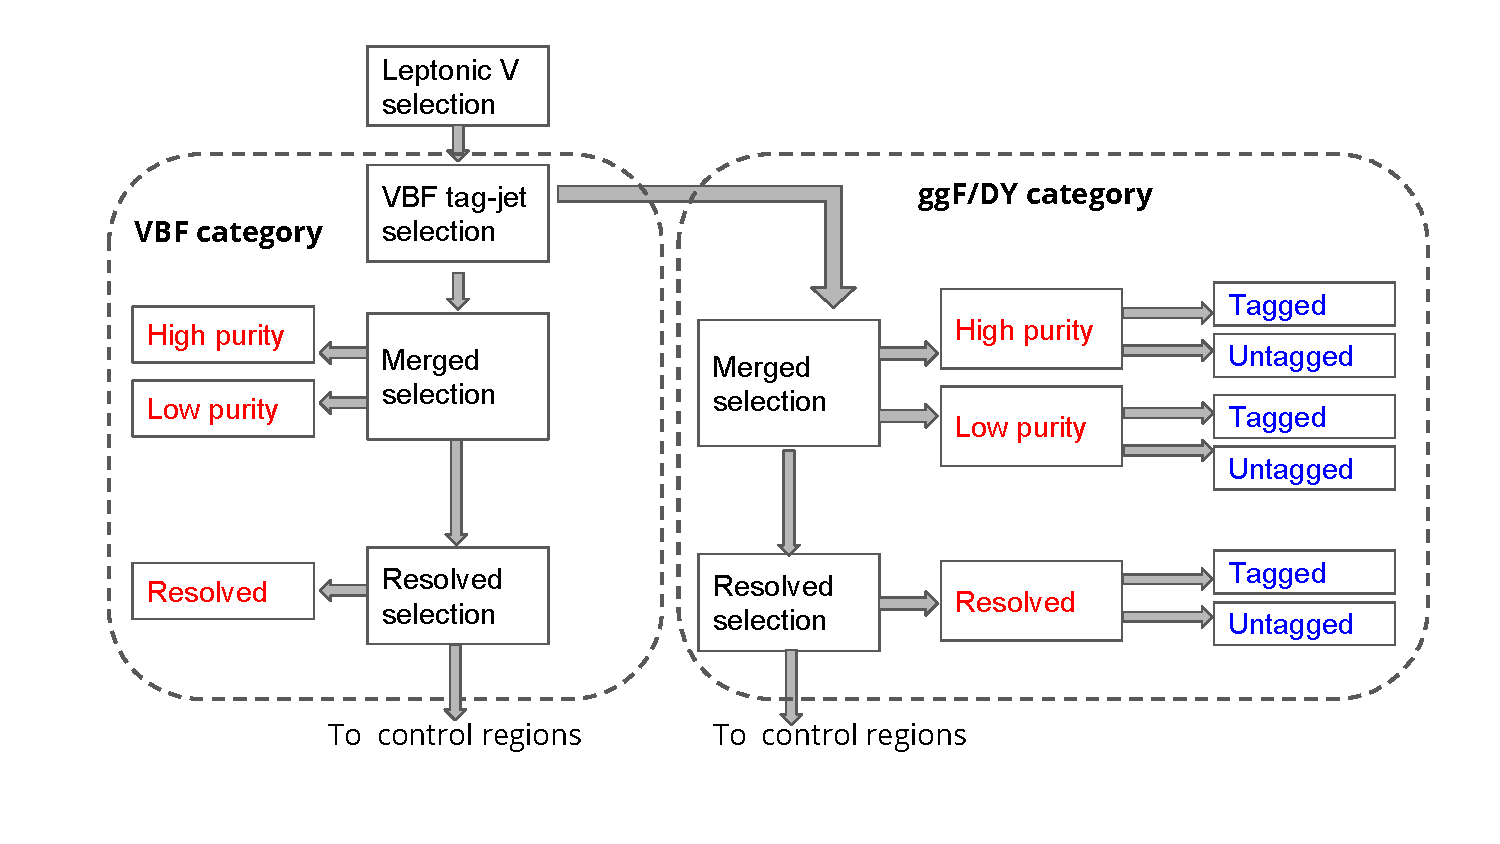
\includegraphics[width=\hsize]{figures/Analysis/cutflow.pdf}  
  \caption{Event Categorization. Natasha write more.} 

  \label{fig:cutflow}
\end{figure} 
\FloatBarrier


\begin{figure}[h!]
  \centering
  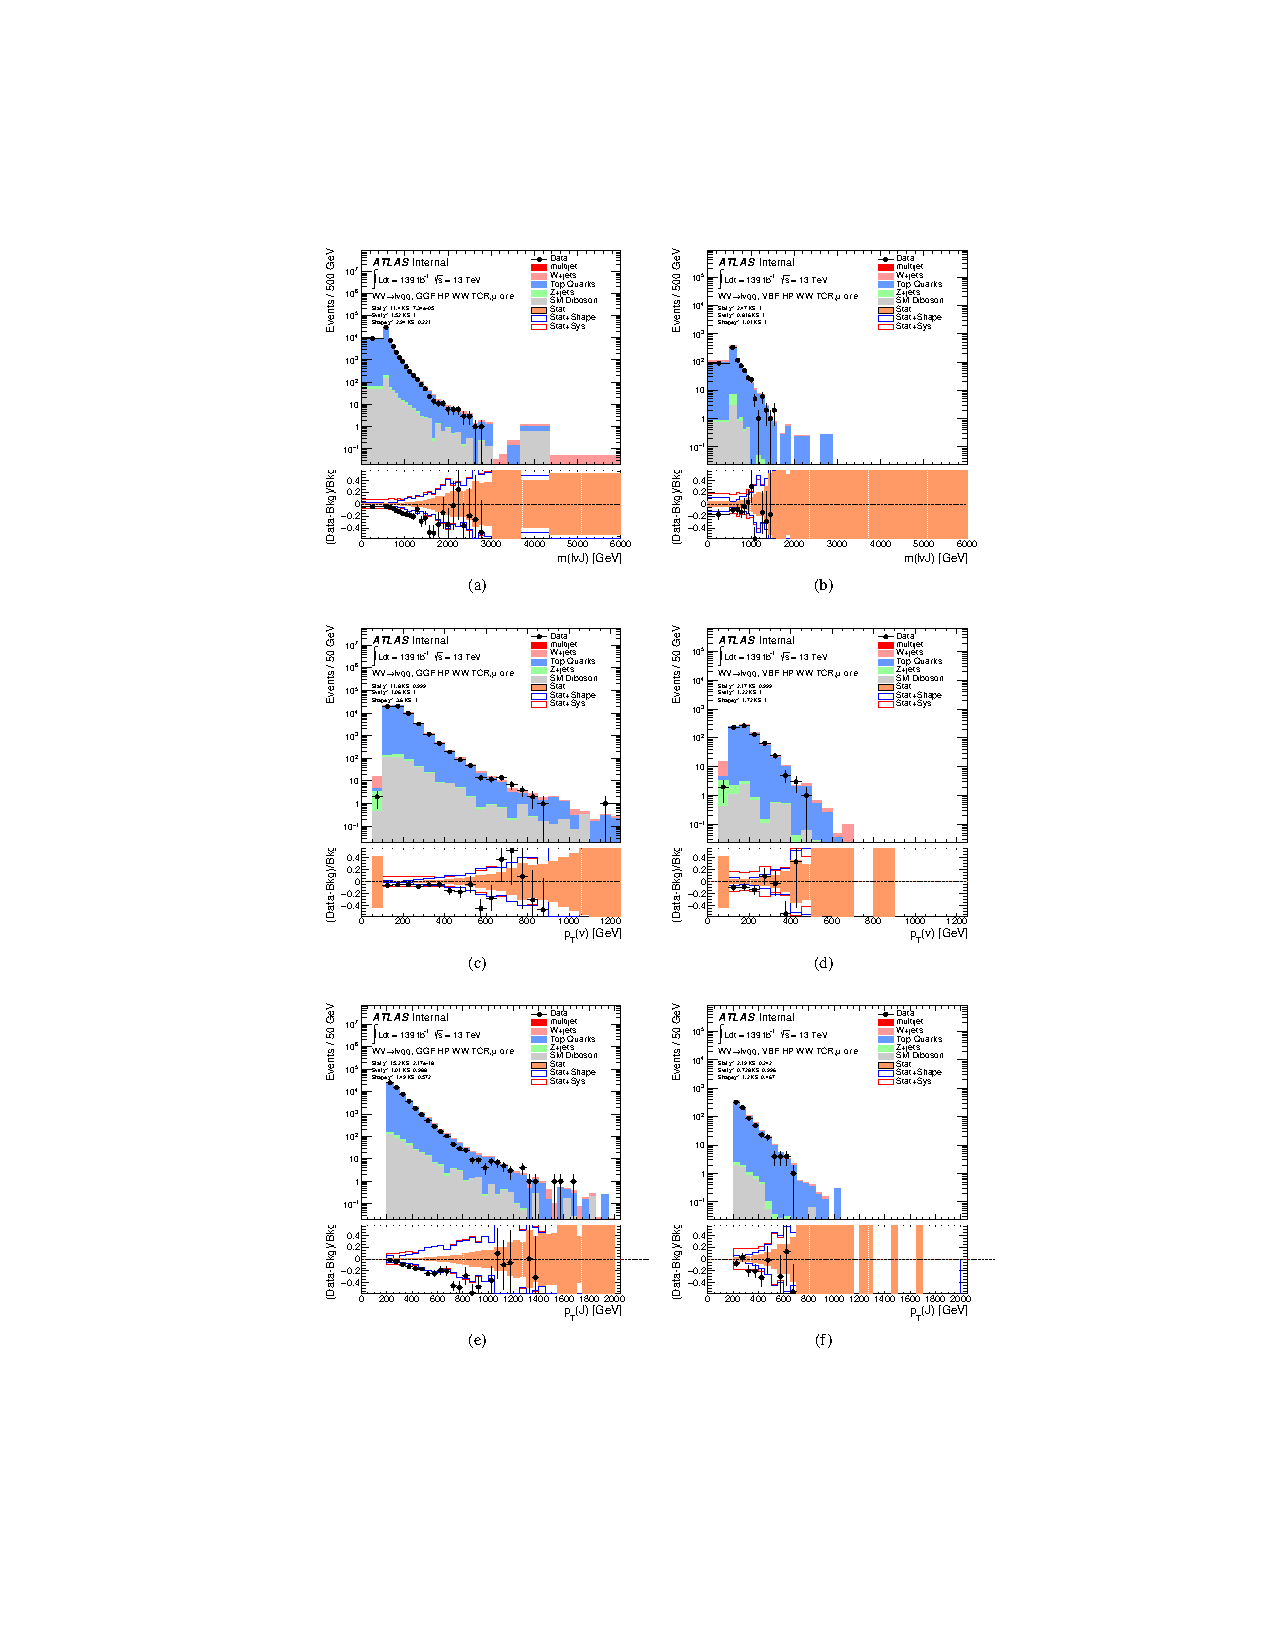
\includegraphics[width=\hsize , height=\textheight , keepaspectratio]{figures/Analysis/datamc/merged_hp_ww_tcr.pdf}
    \caption{Data MC comparison for the merged $WW$ HP TCR. The bottom panel shows the ratio of the difference between data and simulation to simulation. The red bands include the all systematic and statistical uncertainties on the background. } 
  \label{fig:merged_hp_ww_TCR_datamc}
\end{figure} 
\FloatBarrier


\begin{figure}[h!]
  \centering
  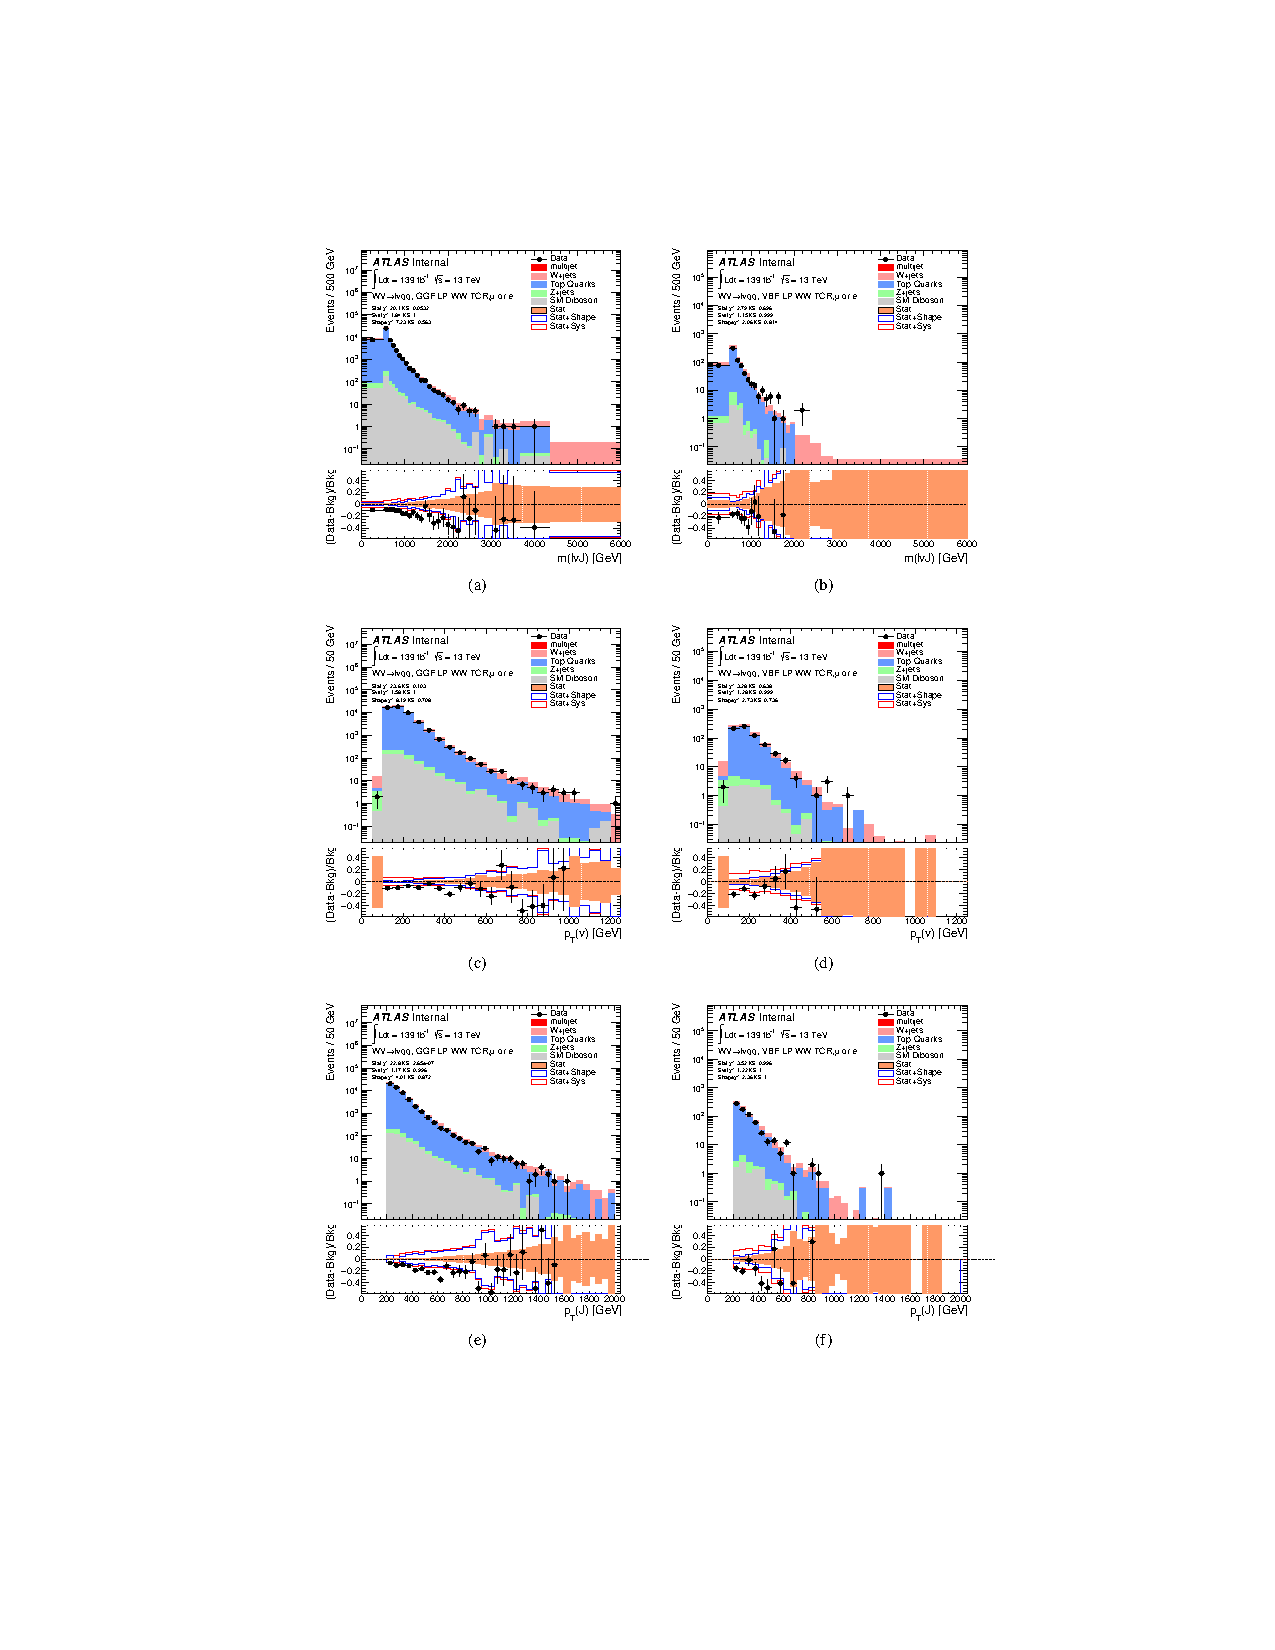
\includegraphics[width=\hsize , height=\textheight , keepaspectratio]{figures/Analysis/datamc/merged_lp_ww_tcr.pdf}
      \caption{Data MC comparison for the merged $WW$ LP TCR. The bottom panel shows the ratio of the difference between data and simulation to simulation. The red bands include the all systematic and statistical uncertainties on the background. } 
  \label{fig:merged_lp_ww_TCR_datamc}
\end{figure} 
\FloatBarrier


\begin{figure}[h!]
  \centering
  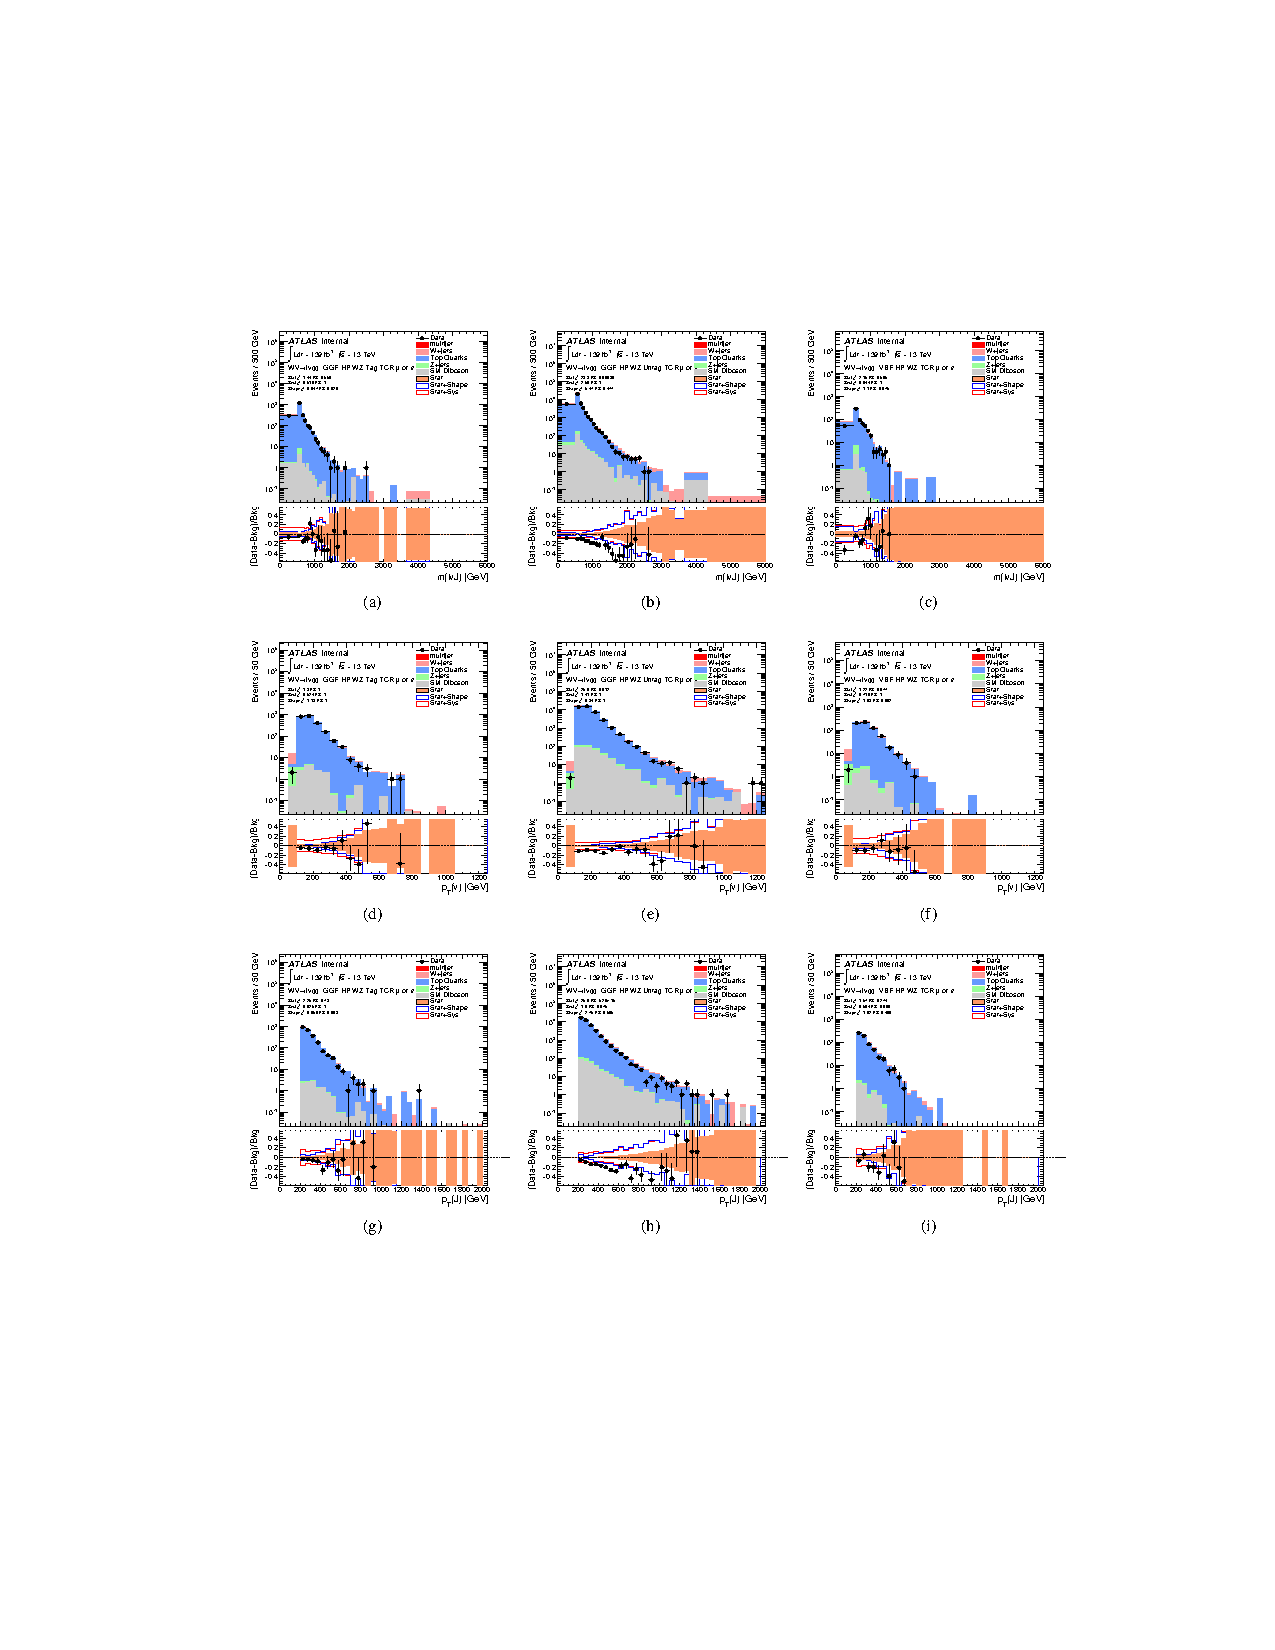
\includegraphics[width=\hsize , height=\textheight , keepaspectratio]{figures/Analysis/datamc/merged_hp_wz_tcr.pdf}
    \caption{Data MC comparison for the merged $WZ$ HP TCR. The bottom panel shows the ratio of the difference between data and simulation to simulation. The red bands include the all systematic and statistical uncertainties on the background. } 
  \label{fig:merged_hp_wz_TCR_datamc}
\end{figure} 
\FloatBarrier


\begin{figure}[h!]
  \centering
  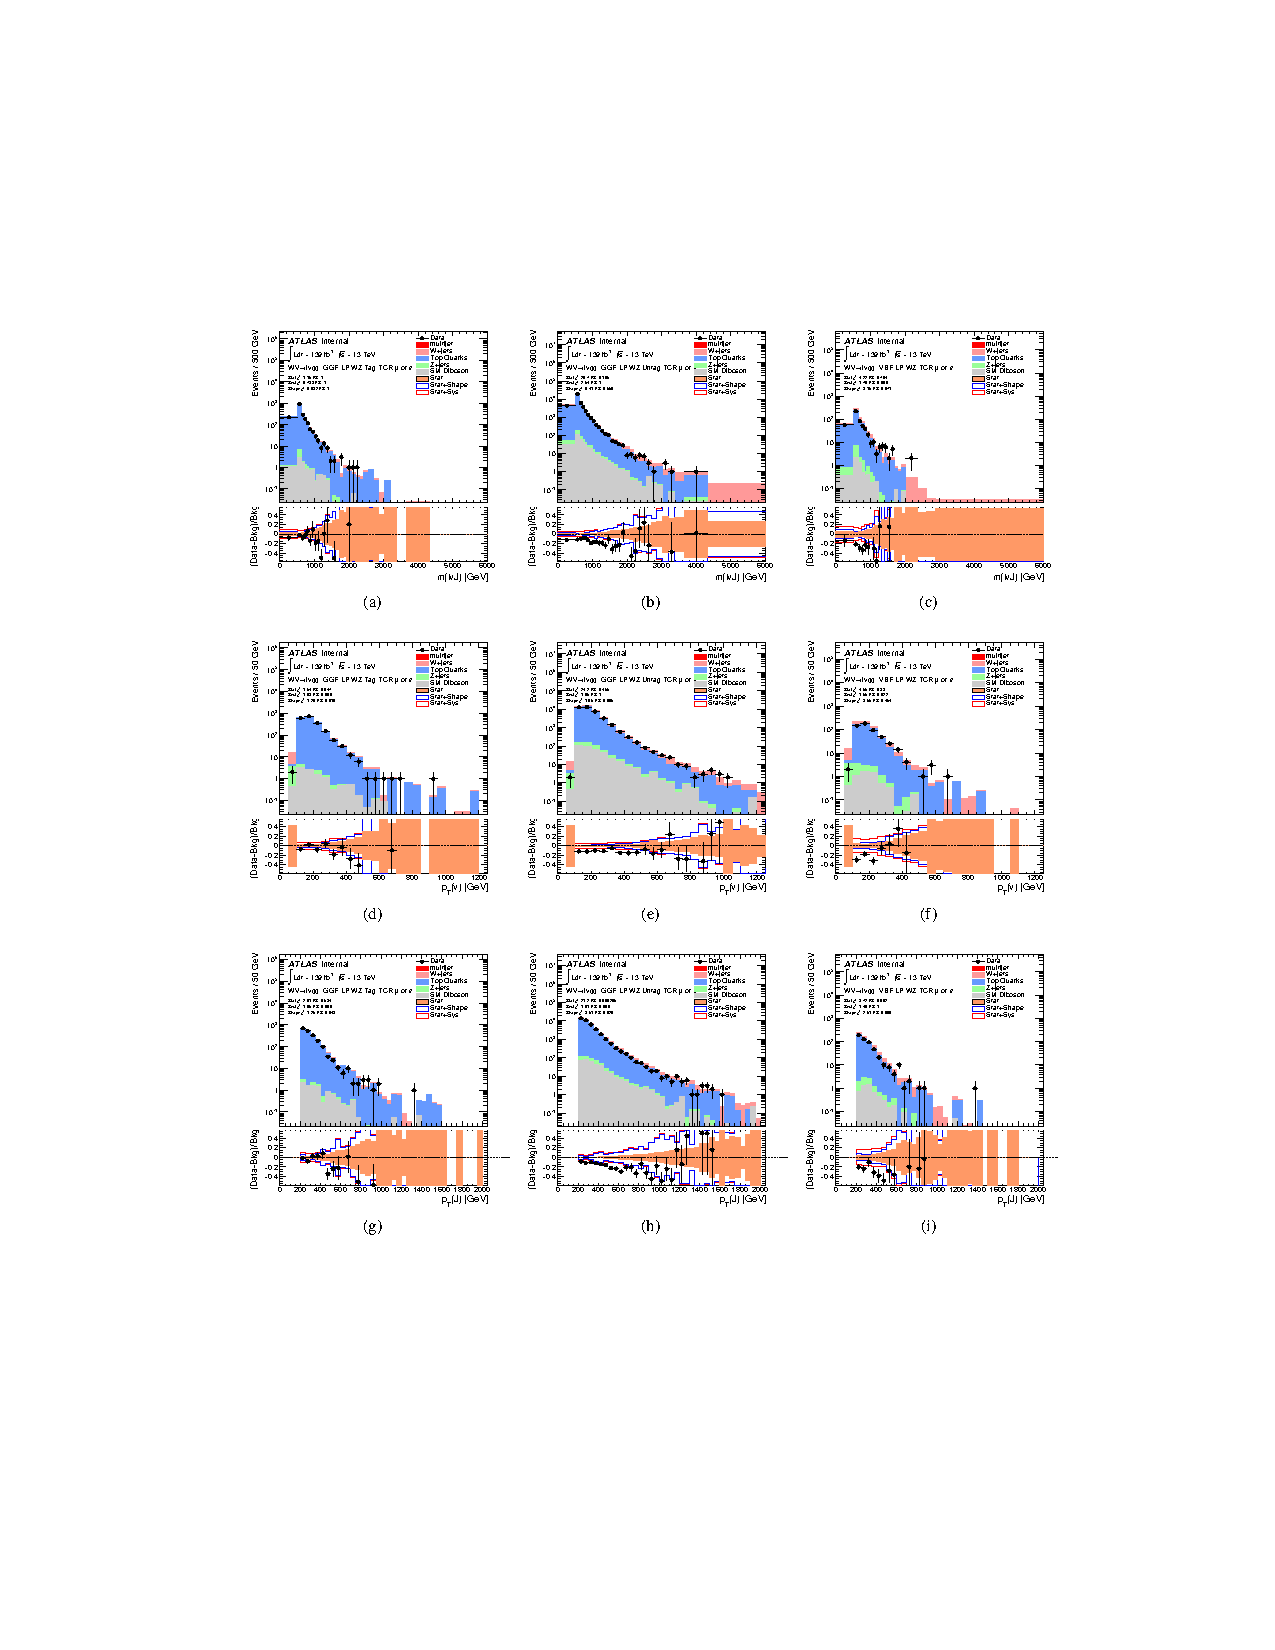
\includegraphics[width=\hsize , height=\textheight , keepaspectratio]{figures/Analysis/datamc/merged_lp_wz_tcr.pdf}
      \caption{Data MC comparison for the merged $WZ$ LP TCR. The bottom panel shows the ratio of the difference between data and simulation to simulation. The red bands include the all systematic and statistical uncertainties on the background. } 
  \label{fig:merged_lp_wz_TCR_datamc}
\end{figure} 
\FloatBarrier


\begin{figure}[h!]
  \centering
  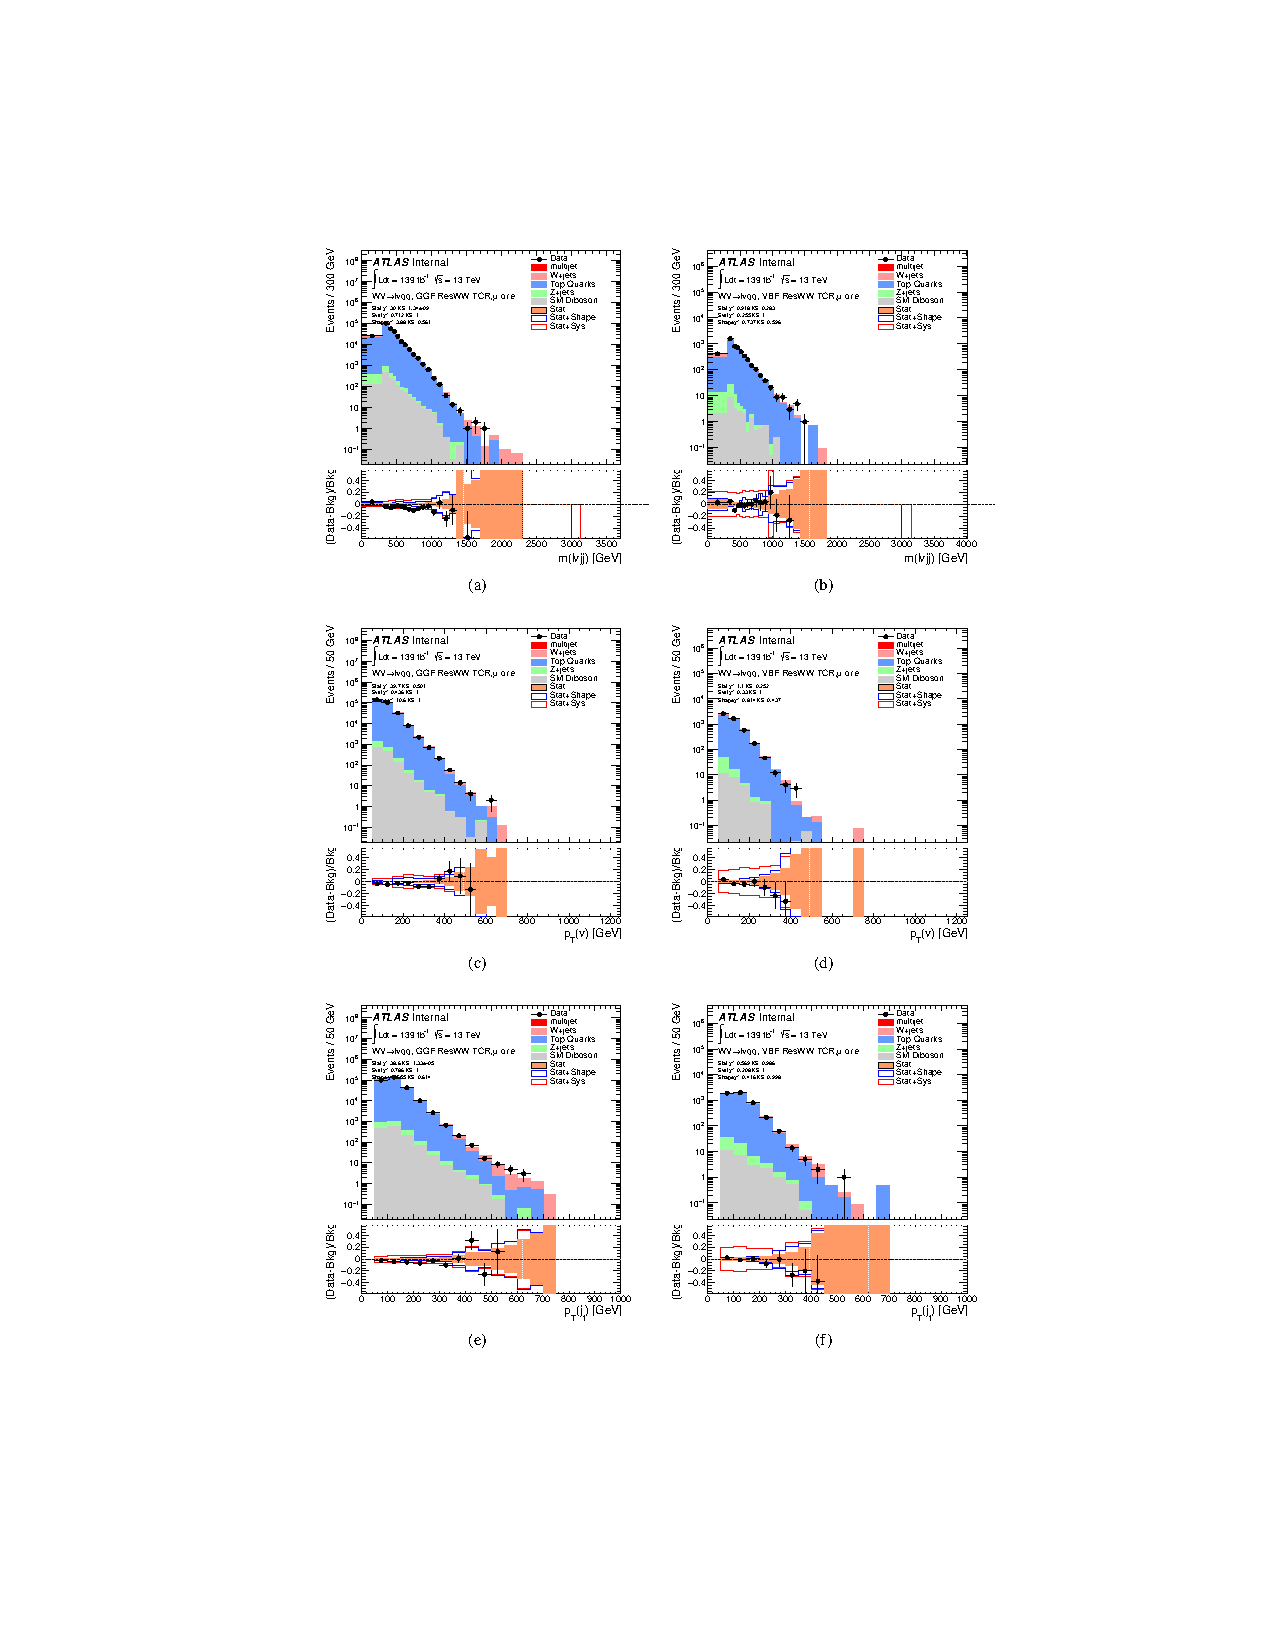
\includegraphics[width=\hsize , height=\textheight , keepaspectratio]{figures/Analysis/datamc/resolved_ww_tcr.pdf}
      \caption{Data MC comparison for the resolved $WW$ TCR. The bottom panel shows the ratio of the difference between data and simulation to simulation. The red bands include the all systematic and statistical uncertainties on the background. } 
  \label{fig:resolved_ww_TCR_datamc}
\end{figure} 
\FloatBarrier


\begin{figure}[h!]
  \centering
  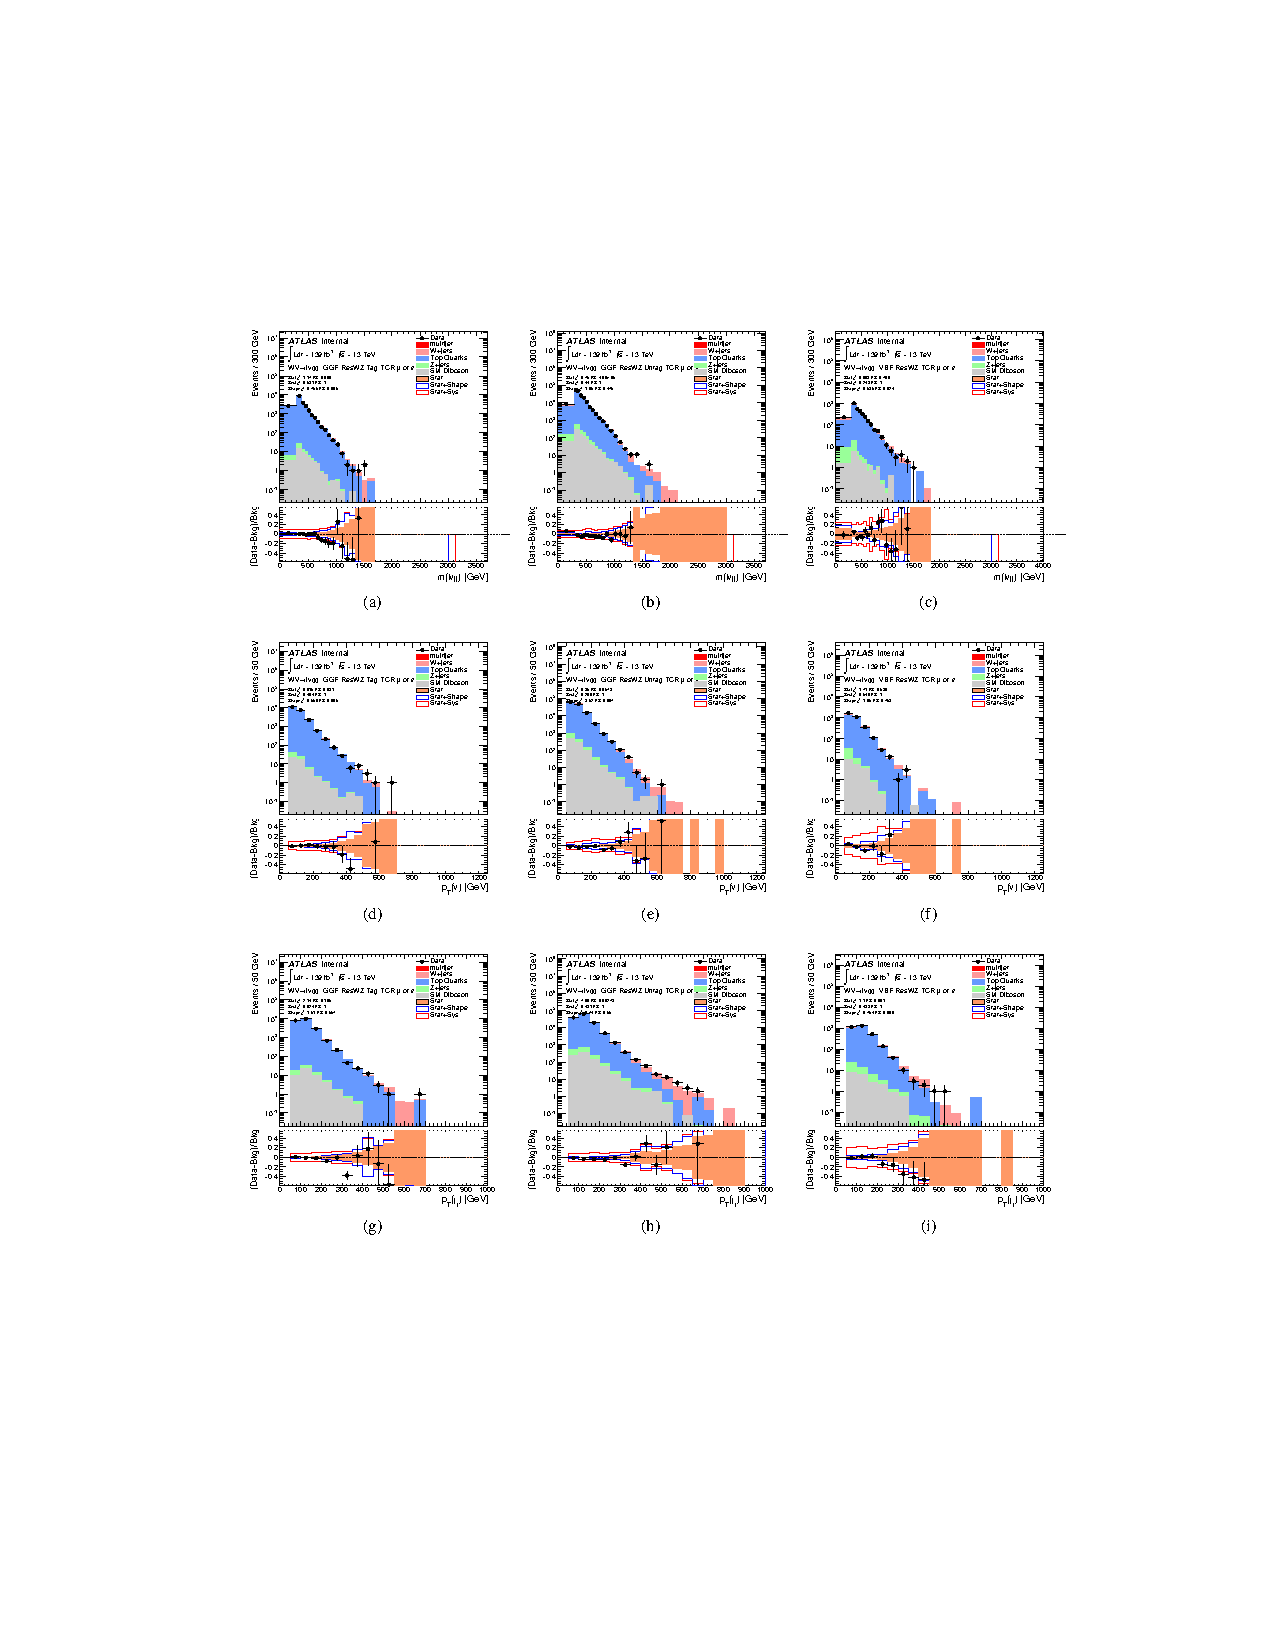
\includegraphics[width=\hsize , height=\textheight , keepaspectratio]{figures/Analysis/datamc/resolved_wz_tcr.pdf}
      \caption{Data MC comparison for the resolved $WZ$ TCR. The bottom panel shows the ratio of the difference between data and simulation to simulation. The red bands include the all systematic and statistical uncertainties on the background. } 
  \label{fig:resolved_wz_TCR_datamc}
\end{figure} 
\FloatBarrier

\section{Selection Acceptance times efficiency for Signal Events}
The acceptance times efficiency for the signal region selection is defined as:

\begin{equation}
A \cdot \epsilon = \frac{N^{\mathrm{truth}}_{\mathrm{events\, selected}}}{N^{\mathrm{truth}}_{\mathrm{events\, generated}}} \cdot \frac{N^{\mathrm{reco}}_{\mathrm{events\, selected}}}{N^{\mathrm{truth}}_{\mathrm{events\, selected}}}
\\
= \frac{N^{\mathrm{reco}}_{\mathrm{events\, selected}}}{N^{\mathrm{truth}}_{\mathrm{events\, generated}}}
\end{equation}
The distributions of $A\cdot \epsilon$ as a function of the resonance mass for the different spin models are shown in Figures \ref{fig:accept_hvtww} - \ref{fig:accept_rsg}.

\begin{figure}[h!]
  \centering
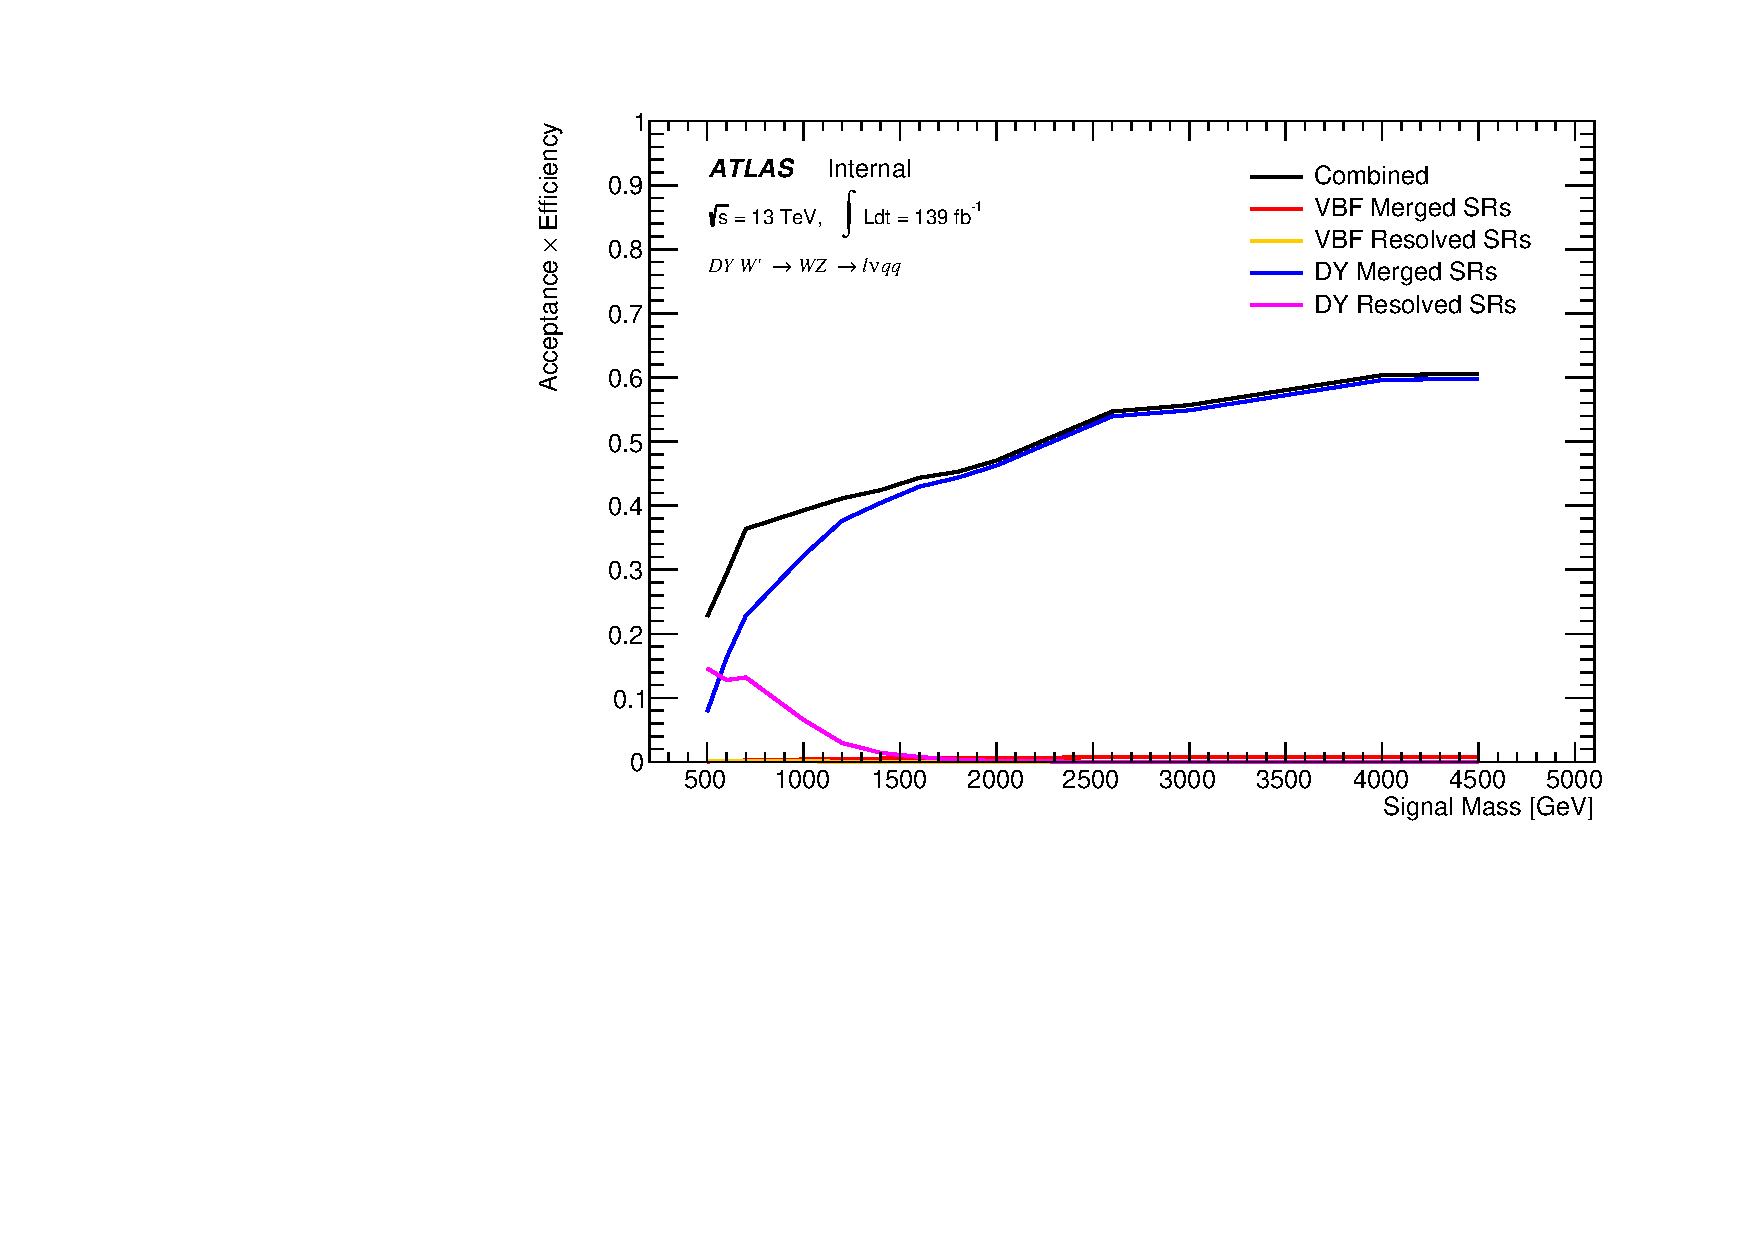
\includegraphics[width=0.48\hsize]{figures/Analysis/signal_acceptance/Acc_times_Eff1lepDYHVT.pdf}
    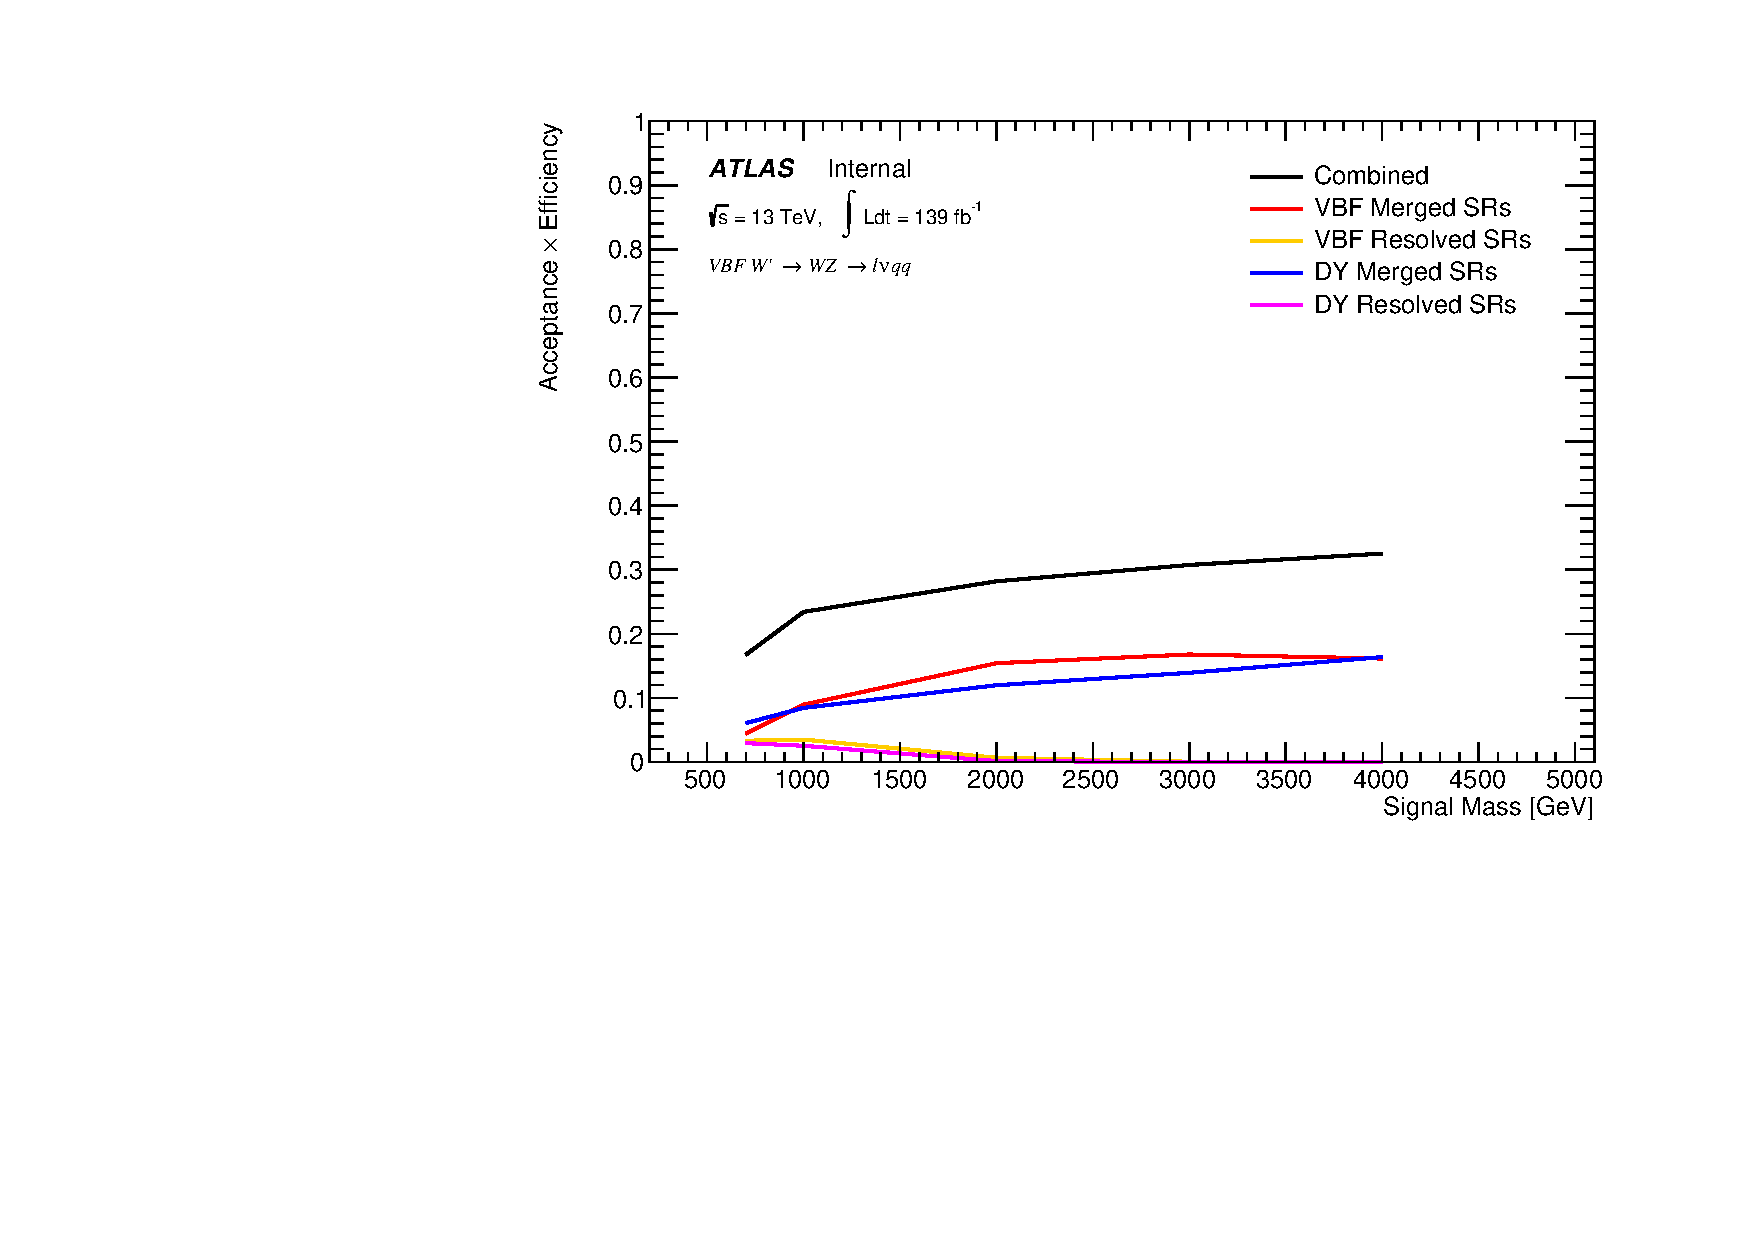
\includegraphics[width=0.48\hsize]{figures/Analysis/signal_acceptance/Acc_times_Eff1lepVBFHVT.pdf}

      \caption{Selection acceptance times efficiency for the $W'\to WZ\to \ell \nu qq$ events from MC simulations as a function of the $W'$ mass for (a) Drell-Yan and (b) VBF production, combining the merged HP and LP signal regions of the $WV\to \ell\nu J$ selection and the resolved regions of the $WV\to \ell\nu jj$ selection.} 
  \label{fig:accept_hvtww}
\end{figure} 
\FloatBarrier


\begin{figure}[h!]
  \centering
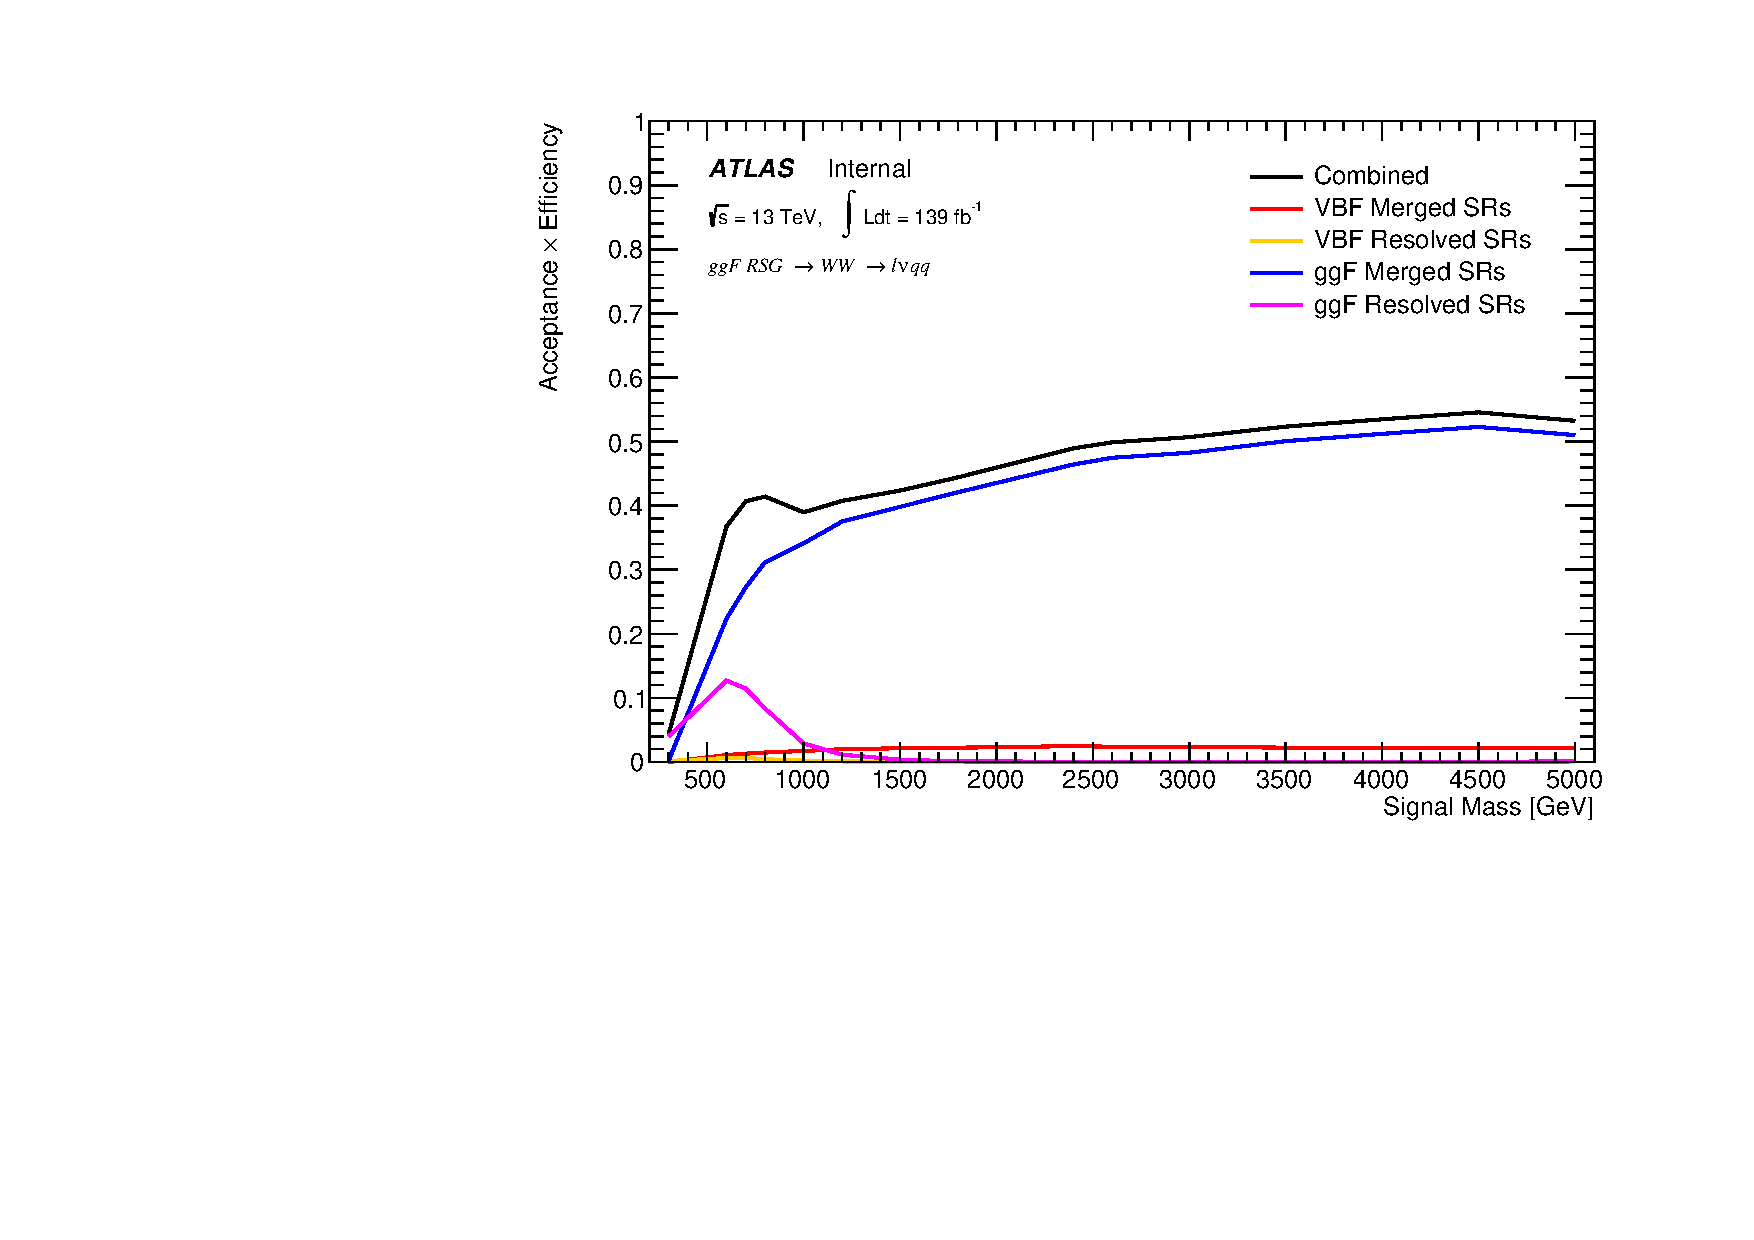
\includegraphics[width=0.48\hsize]{figures/Analysis/signal_acceptance/Acc_times_Eff1lepggFRSG.pdf}
    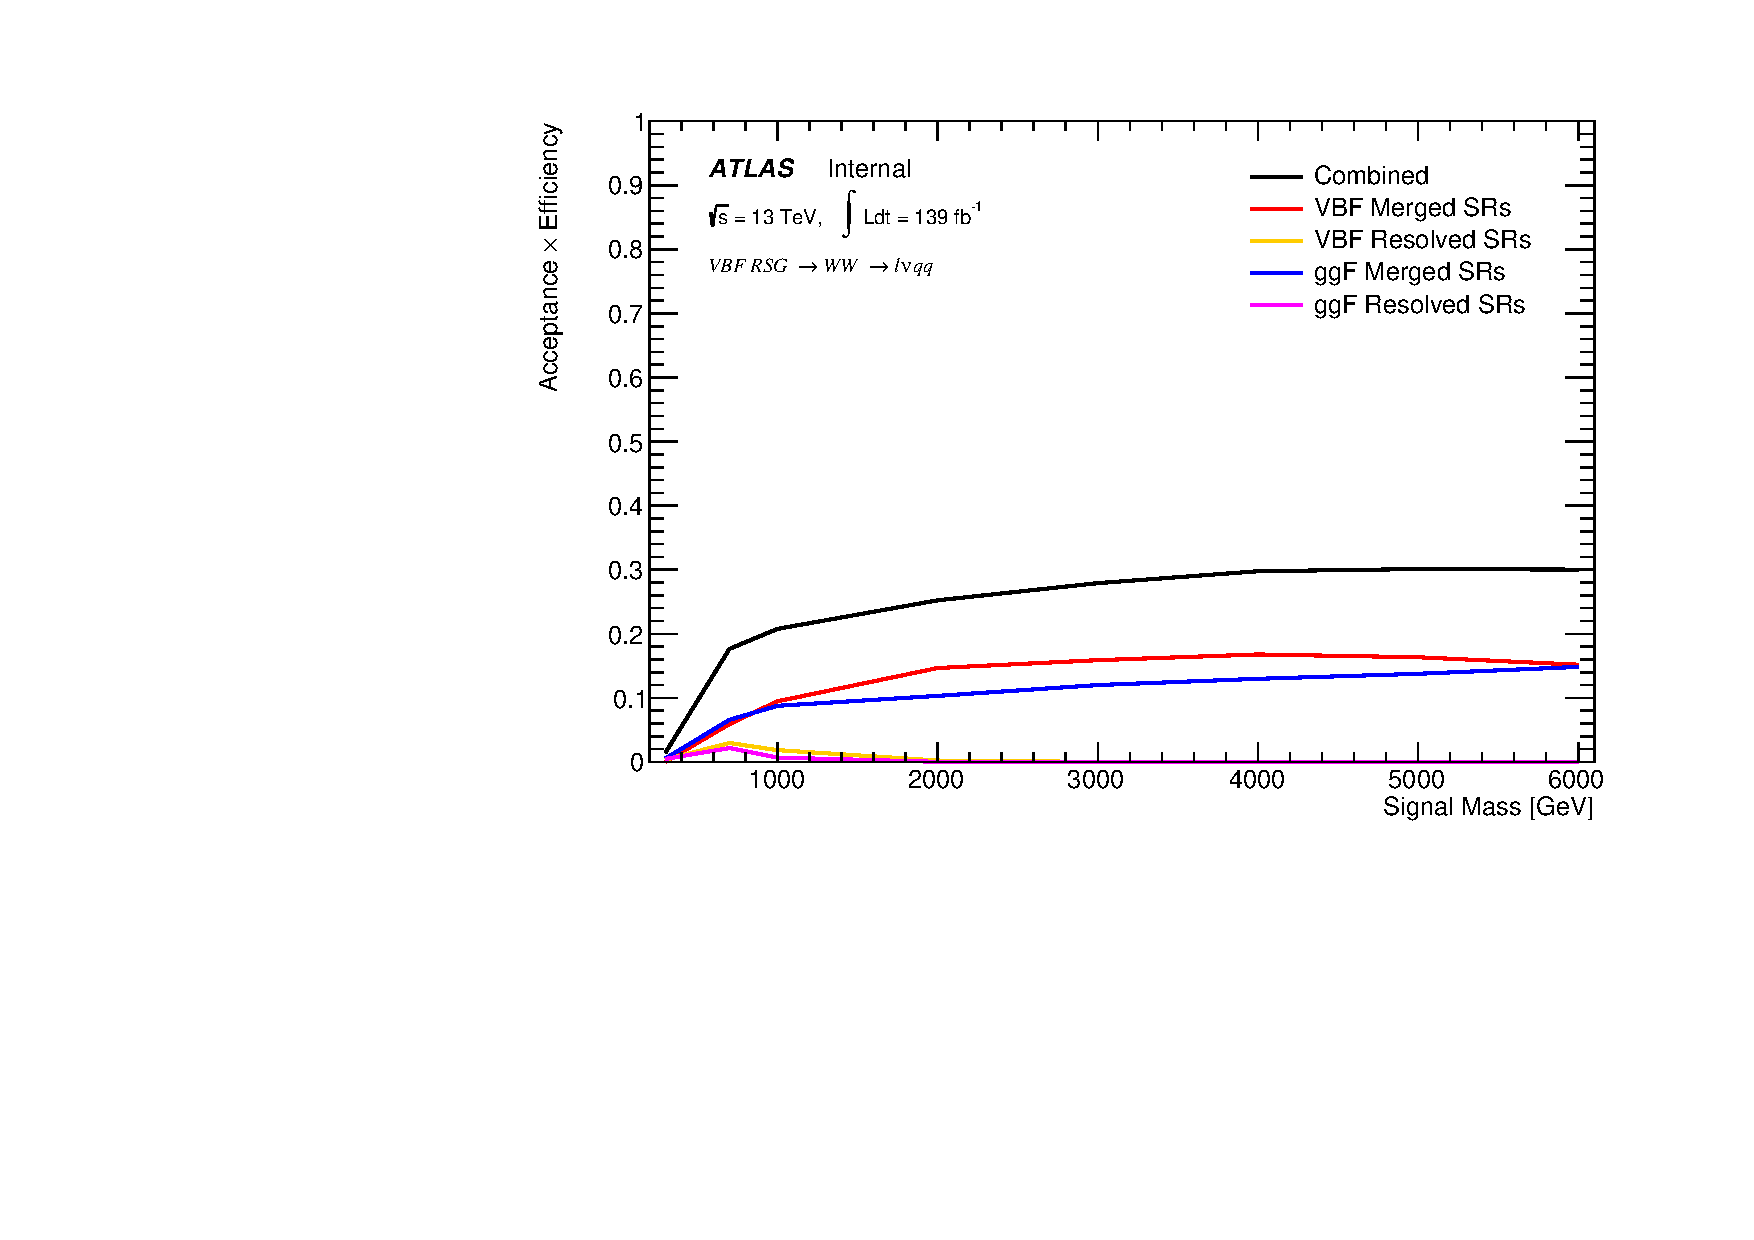
\includegraphics[width=0.48\hsize]{figures/Analysis/signal_acceptance/Acc_times_Eff1lepVBFRSG.pdf}

      \caption{Selection acceptance times efficiency for the $G\to WW\to \ell \nu qq$ events from MC simulations as a function of the $G$ mass for (a) Drell-Yan and (b) VBF production, combining the merged HP and LP signal regions of the $WV\to \ell\nu J$ selection and the resolved regions of the $WV\to \ell\nu jj$ selection.} 
  \label{fig:accept_hvtww}
\end{figure} 
\FloatBarrier
\section{Background Estimate}
\subsection{Control Regions}
To more accurately model the two dominant backgrounds in this analysis, $W$+jets and $t\bar{t}$, control regions are constructed for each. These control regions are dominated by these processes and used to extract normalization factors in the final likelihood fit that are then used in the signal region estimates. For the $t\bar{t}$ control region the event must contain at least one such b jet. The WCR is constructed using the $m_{jj/J}$ mass window sidebands. All other backgrounds are estimated using simulation, except fake lepton backgrounds, which are derived using a data-driven method.
\subsection{Fake Lepton Backgrounds}
Backgrounds in this analysis containing real leptons (e.g. $W/Z$+jets, diboson, $t\bar{t}$, single-$t$) are well-modeled with simulated samples and constrained with data from CRs. However, the fake lepton background (also referred to as the multijet background) is not well-modeled with simulation. For this reason, the multijet background is extracted from data. Heavy flavor decay products, jets, and converted photons can be mistakenly reconstructed as electrons. Fake electrons often arise from jet fakes while non-prompt muons usually arise from heavy flavor decay.  For this analysis, these fake electrons generally fail the electron ID criteria and fake muons fail the muon isolation requirement. Therefore, to derive the multijet template shape the SR and CR selections and inverted lepton requirements are used as seen in Table \ref{tab:TempMJCR}. NB: by inverting the lepton isolation/identification criteria the SRs and CRs are orthogonal.

The template shape of the MJ background is determined by using a multijet validation region (MJVR) that requires the inverted lepton isolation/identification requirement and the two signal jets to satisfy the $m_{jj}$ requirement used in the $W$+jets CRs. The $E_{T}^{miss}$ distribution in MJCR is shown in Figure \ref{fig:multijet_met} for 2017 data. The template is then extracted by subtracting the data in the MJVR from the electroweak background processes. The resulting template and electroweak backgrounds are then fit to data. In this fit, the $E_{T}^{miss}$ distribution compared to data to extract electroweak background, multijet electron and muon background normalizations.  The fitted scale factors from this MJVR template are then applied in the MJCR template. The electron and muon background normalizations in the MJCR template are parameters in the final simultaneous fit. Technically, there should be a separate template for every CR and SR, but some MJ regions have insufficient statistics to do this. Additionally, the shapes for the MJ templates for VBF and ggF regions are found to be compatible within statistical uncertainty. Therefore, the sample MJ template used for VBF and ggF CR/SRs, but with different pre-MJ-fit scale factors. 

This template method was validated using WCR and full Run 2 data. The results of the fit are shown in Table \ref{tab:template_validation_CR}. The multijet contribution in the muon channel for $p_{T}^{W} > 150$ GeV is consistent with zero, and therefore neglected in the final fit. Applying the extracted normalization factor to MJVR in WCRs for various kinematic variables such as $E_{T}^{miss}$, $W$ transverse mass, lepton $p_{T}$, and the invariant mass as show in Figures \ref{fig:multijet_met_elec_ww} -\ref{fig:multijet_met_muon_wz_vbf}. These figures show good agreement between the data and background estimate.

\begin{center}
  \begin{table}[ht]
  \centering
    \caption{Definitions of ``inverted'' leptons used in multijet control region}
  \small
  \begin{tabular}{|l|l|l|l|}
         \hline
         & Criterion       & signal lepton                        & inverted lepton
         \\
         \hline
  Electron & ID              & TightLH                   & \begin{tabular}[c]{@{}l@{}}MediumLH\\ !TightLH\end{tabular} \\
         & Calo Isolation  & FixedCutHighPtCaloOnlyIso  & FixedCutHighPtCaloOnlyIso                                                                           \\ \hline
  Muon   & ID              & WHSignalMuon              & WHSignalMuon                                                                                        \\
         & Track Isolation & FixedCutTightTrackOnlyIso  & \begin{tabular}[c]{@{}l@{}}!FixedCutTightTrackOnlyIso\\ $ptvarcone30/pt<0.07^{*}$\end{tabular}\\ \hline
         &\multicolumn{3}{c|}{\small{ *Only applied to events with $pTW < 150GeV$}} \\ \hline 
  \end{tabular}

  \label{tab:TempMJCR}
  \end{table}
\end{center}

\begin{figure}[h!]
  \centering
  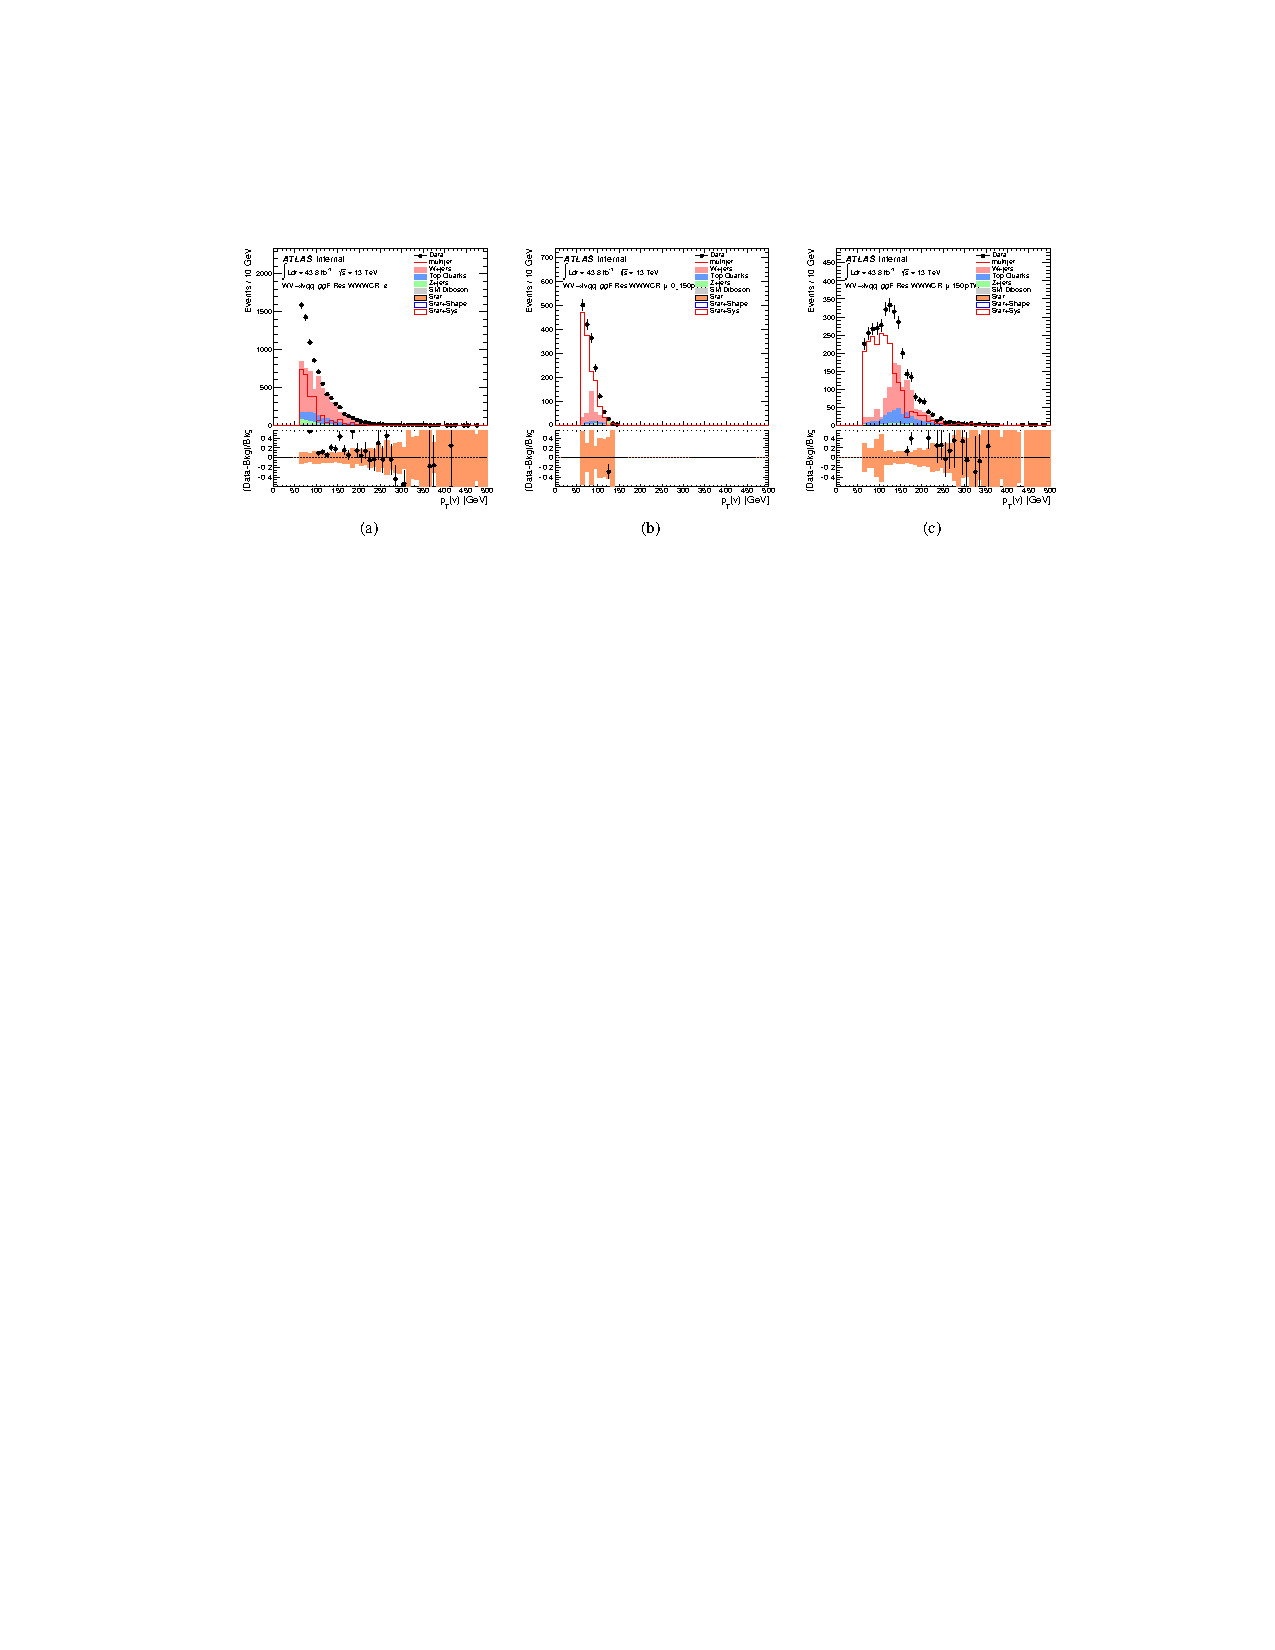
\includegraphics[width=\hsize]{figures/Analysis/multijet/multijet_met.pdf}
      \caption{The $E_{T}^{miss}$ distribution in MJCR for 2017 data in the electron channel(left), muon channel with W-boson pT < 150 GeV (center) and > 150 GeV (right). Multi-jet templates are calculated as remaining data components after excluding known MC} 
  \label{fig:multijet_met}
\end{figure} 
\FloatBarrier



\begin{figure}[h!]
  \centering
  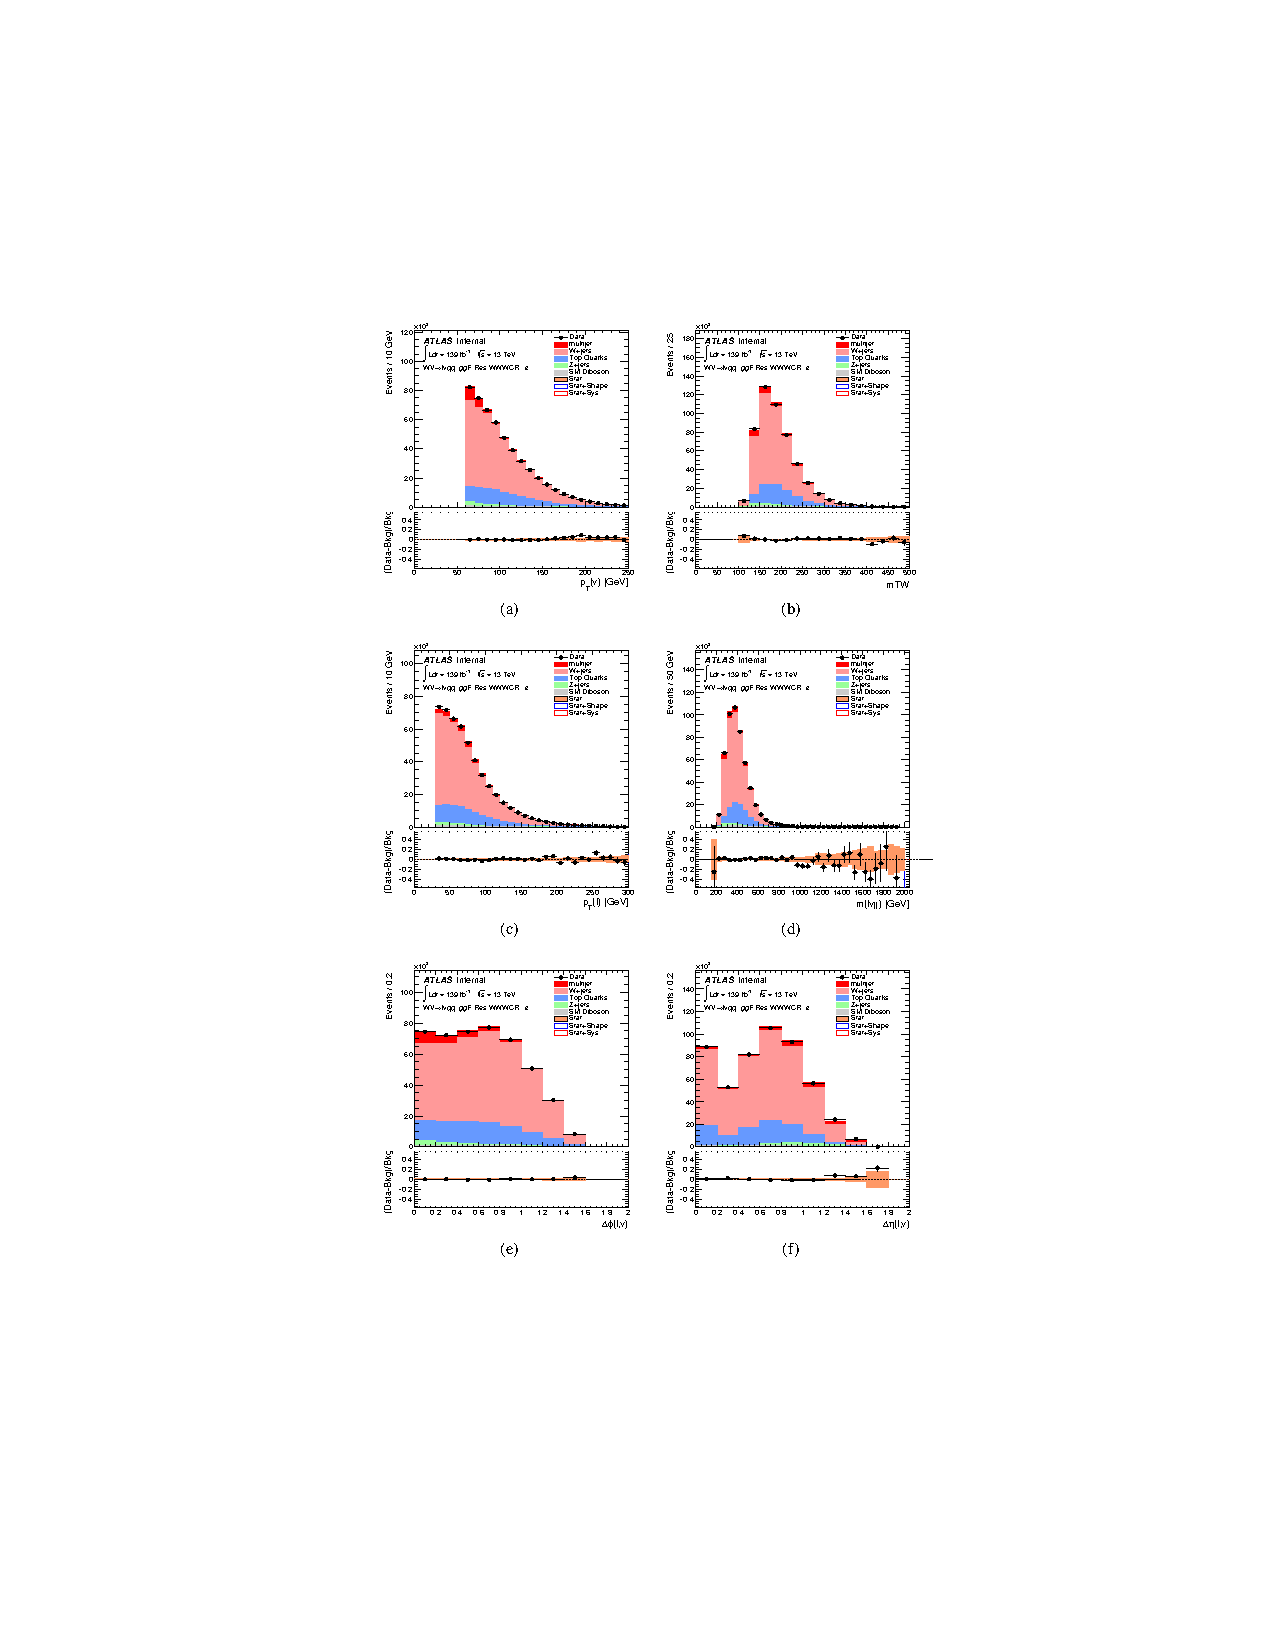
\includegraphics[width=\hsize , height=\textheight , keepaspectratio]{figures/Analysis/multijet/mj_elec_ww.pdf}
      \caption{Postfit Data/MC comparison of distributions of $E_{T}^{miss}$, $m_{T}^{W}$, lepton and neutrino $p_{T}$, $m_{\ell \nu jj}$, lepton-$\nu$ angular distance in the $WW$ electron channel. The MJ template is obtained from the pre-MJ-fit.} 
  \label{fig:multijet_met_elec_ww}
\end{figure} 
\FloatBarrier


\begin{figure}[h!]
  \centering
  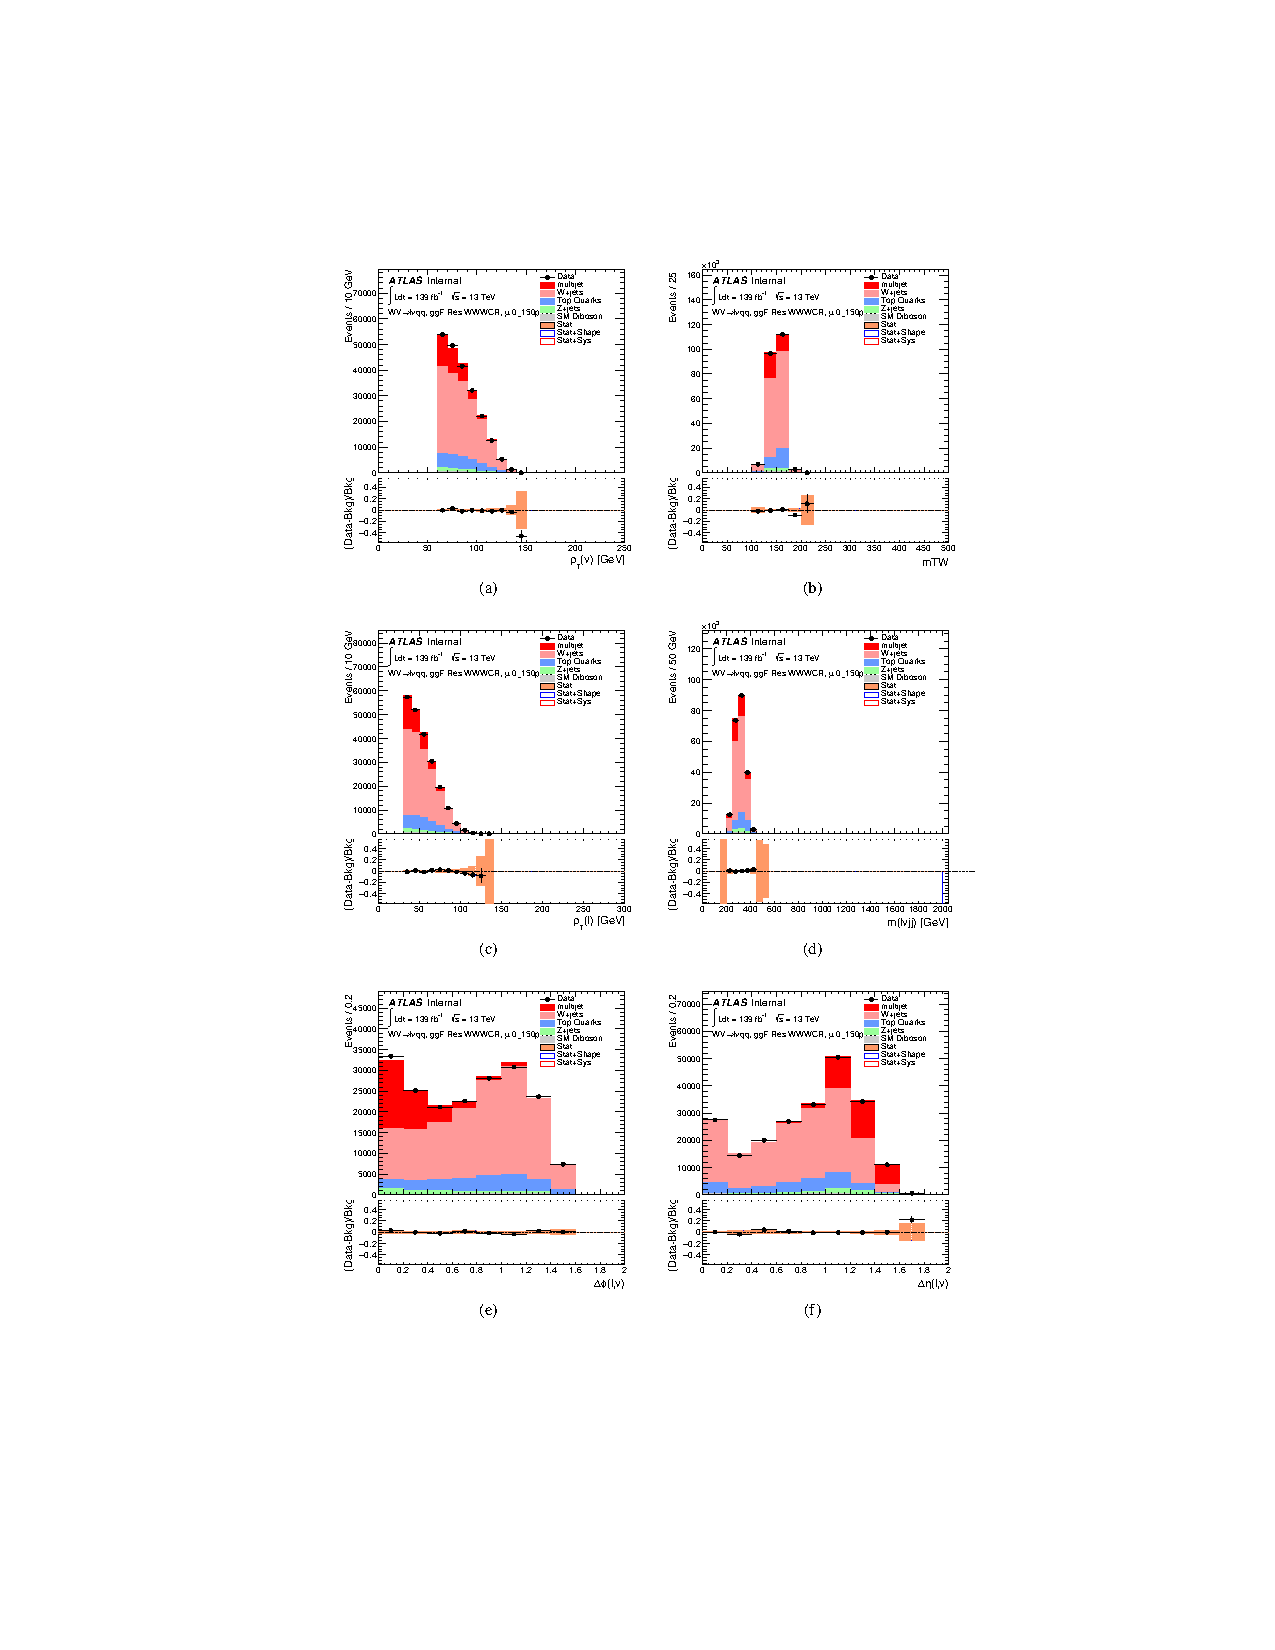
\includegraphics[width=\hsize , height=\textheight , keepaspectratio]{figures/Analysis/multijet/mj_muon_ww.pdf}
      \caption{Postfit Data/MC comparison of distributions of $E_{T}^{miss}$, $m_{T}^{W}$, lepton and neutrino $p_{T}$, $m_{\ell \nu jj}$, lepton-$\nu$ angular distance in the $WW$ muon channel. The MJ template is obtained from the pre-MJ-fit.} 
  \label{fig:multijet_met_muon_ww}
\end{figure} 
\FloatBarrier



\begin{figure}[h!]
  \centering
  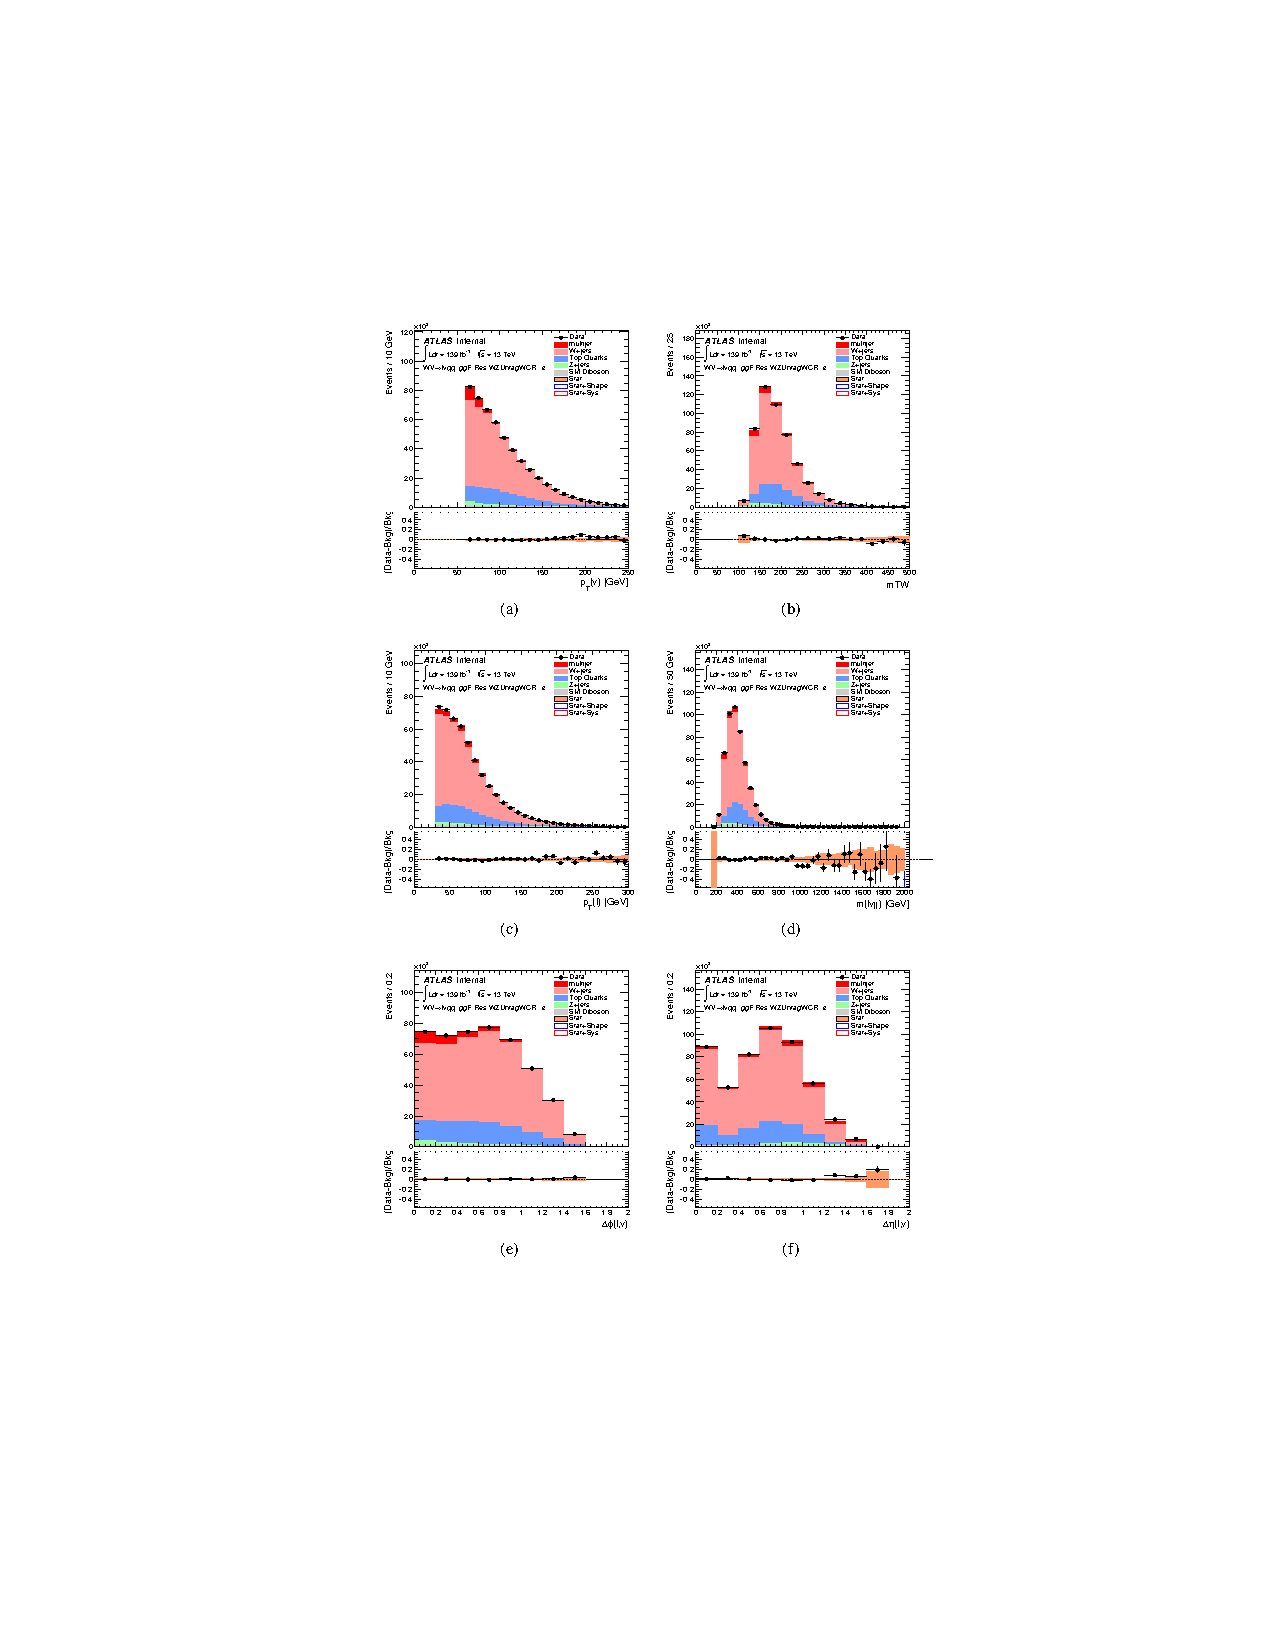
\includegraphics[width=\hsize , height=\textheight , keepaspectratio]{figures/Analysis/multijet/mj_elec_wz_untag.pdf}
      \caption{Postfit Data/MC comparison of distributions of $E_{T}^{miss}$, $m_{T}^{W}$, lepton and neutrino $p_{T}$, $m_{\ell \nu jj}$, lepton-$\nu$ angular distance in the $WZ$ untag electron channel. The MJ template is obtained from the pre-MJ-fit.} 
  \label{fig:multijet_met_elec_wz_untag}
\end{figure} 
\FloatBarrier


\begin{figure}[h!]
  \centering
  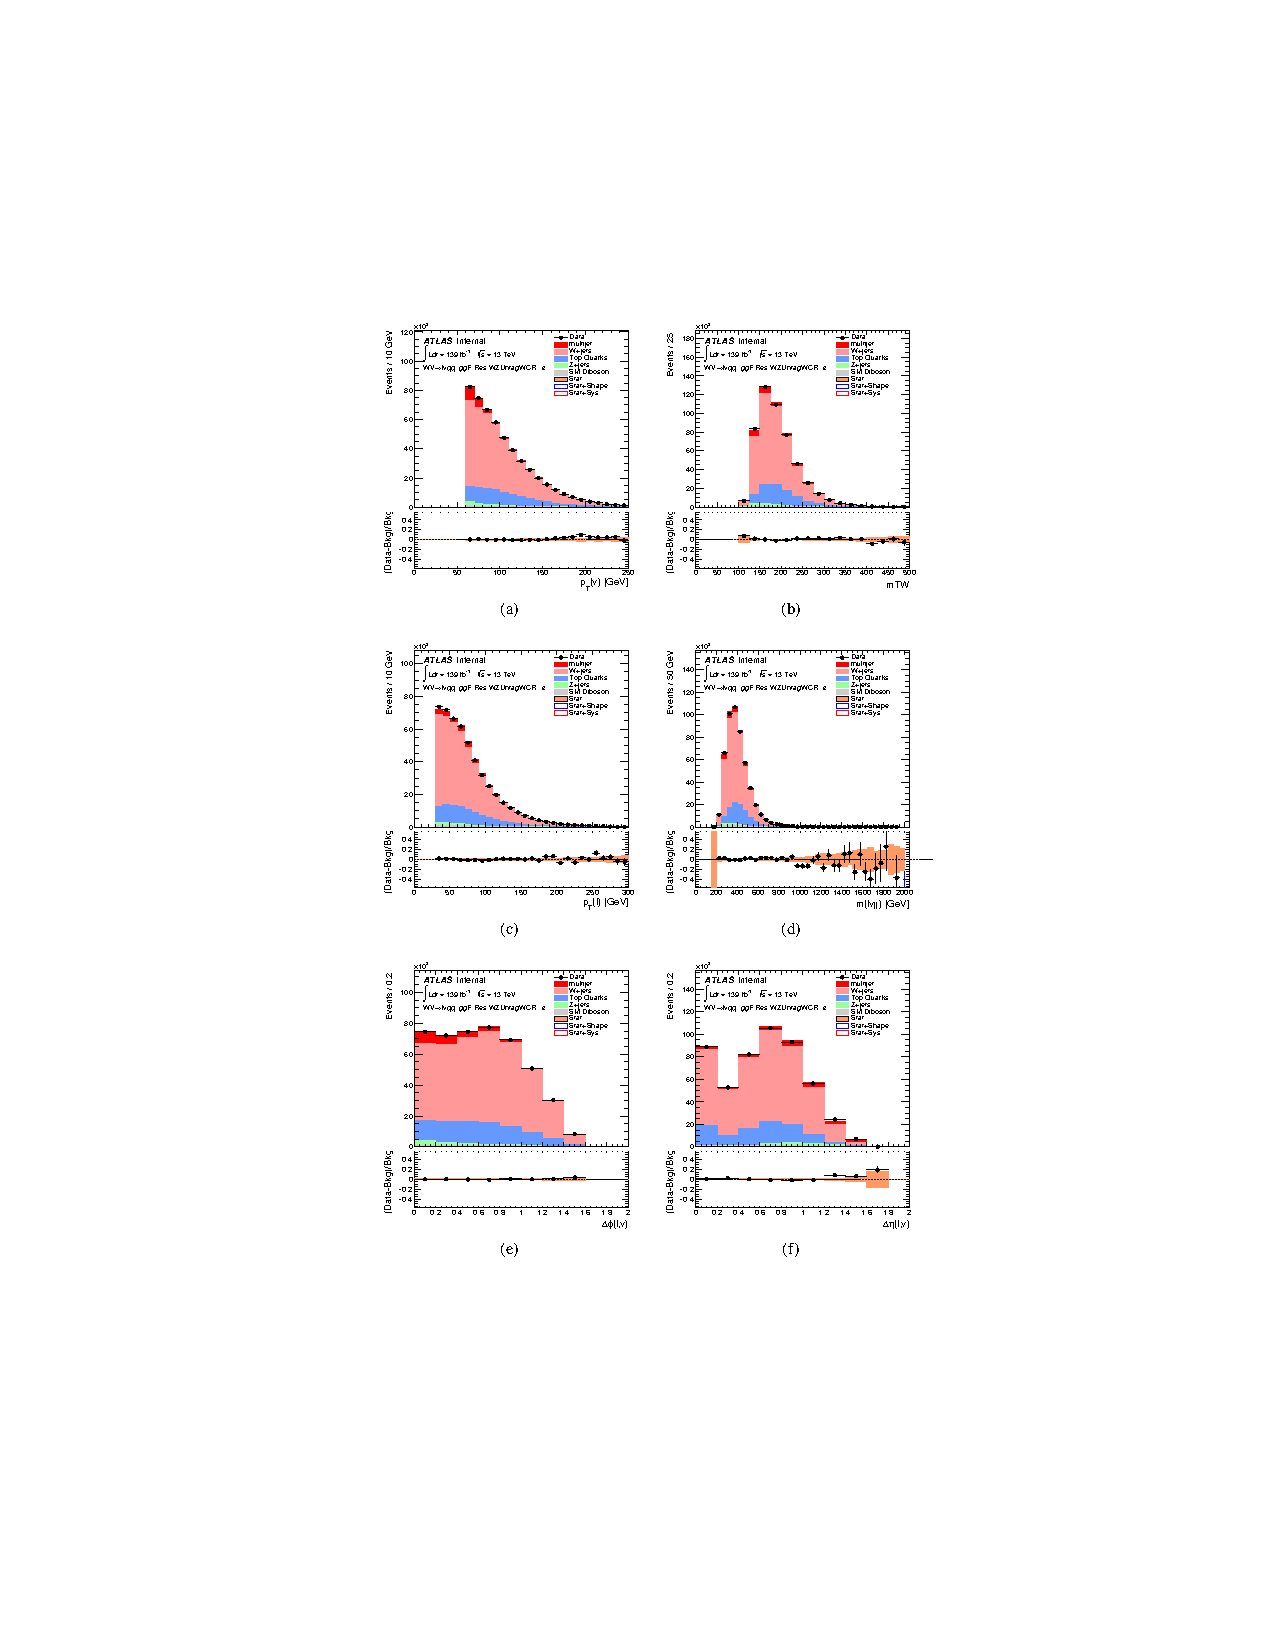
\includegraphics[width=\hsize , height=\textheight , keepaspectratio]{figures/Analysis/multijet/mj_muon_wz_untag.pdf}
      \caption{Postfit Data/MC comparison of distributions of $E_{T}^{miss}$, $m_{T}^{W}$, lepton and neutrino $p_{T}$, $m_{\ell \nu jj}$, lepton-$\nu$ angular distance in the $WZ$ untag muon channel. The MJ template is obtained from the pre-MJ-fit.} 
  \label{fig:multijet_met_muon_wz_untag}
\end{figure} 
\FloatBarrier


\begin{figure}[h!]
  \centering
  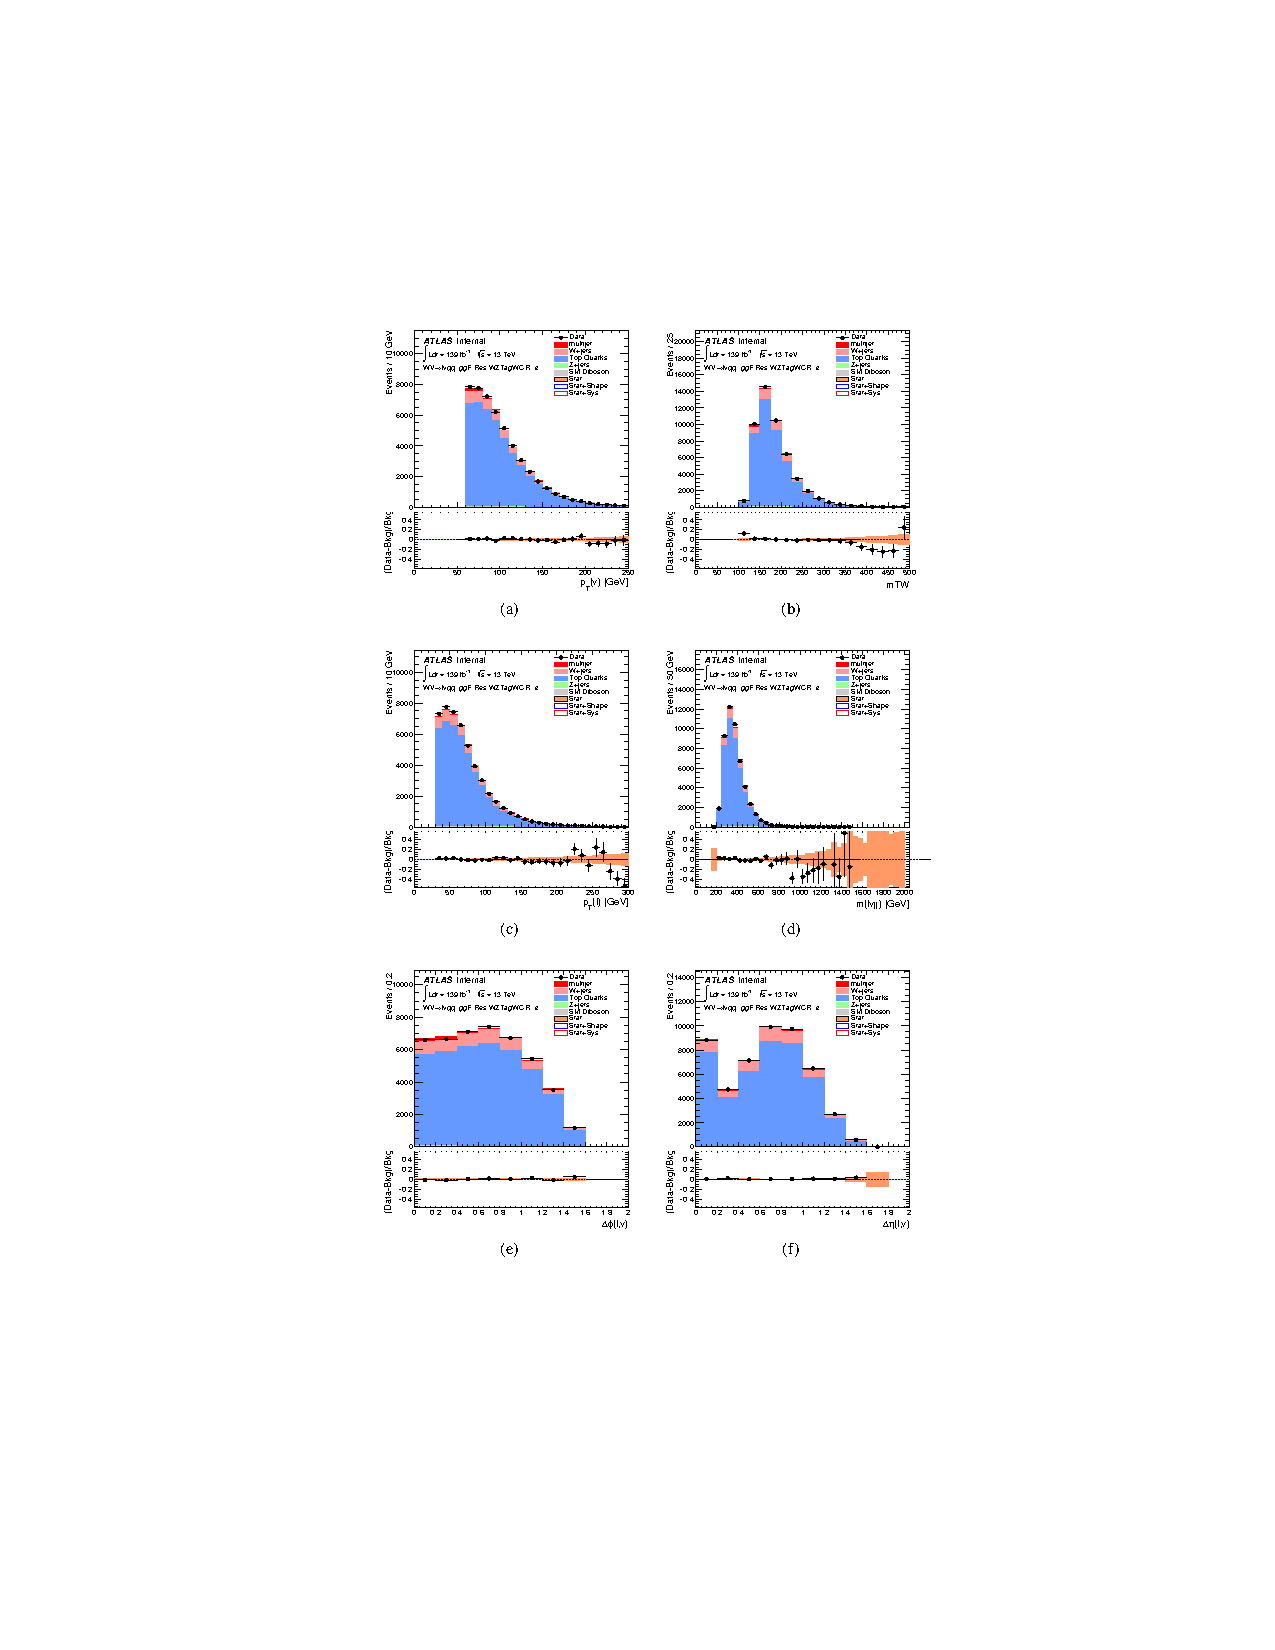
\includegraphics[width=\hsize , height=\textheight , keepaspectratio]{figures/Analysis/multijet/mj_elec_wz_tag.pdf}
      \caption{Postfit Data/MC comparison of distributions of $E_{T}^{miss}$, $m_{T}^{W}$, lepton and neutrino $p_{T}$, $m_{\ell \nu jj}$, lepton-$\nu$ angular distance in the $WZ$ untag electron channel. The MJ template is obtained from the pre-MJ-fit.} 
  \label{fig:multijet_met_elec_wz_untag}
\end{figure} 
\FloatBarrier


\begin{figure}[h!]
  \centering
  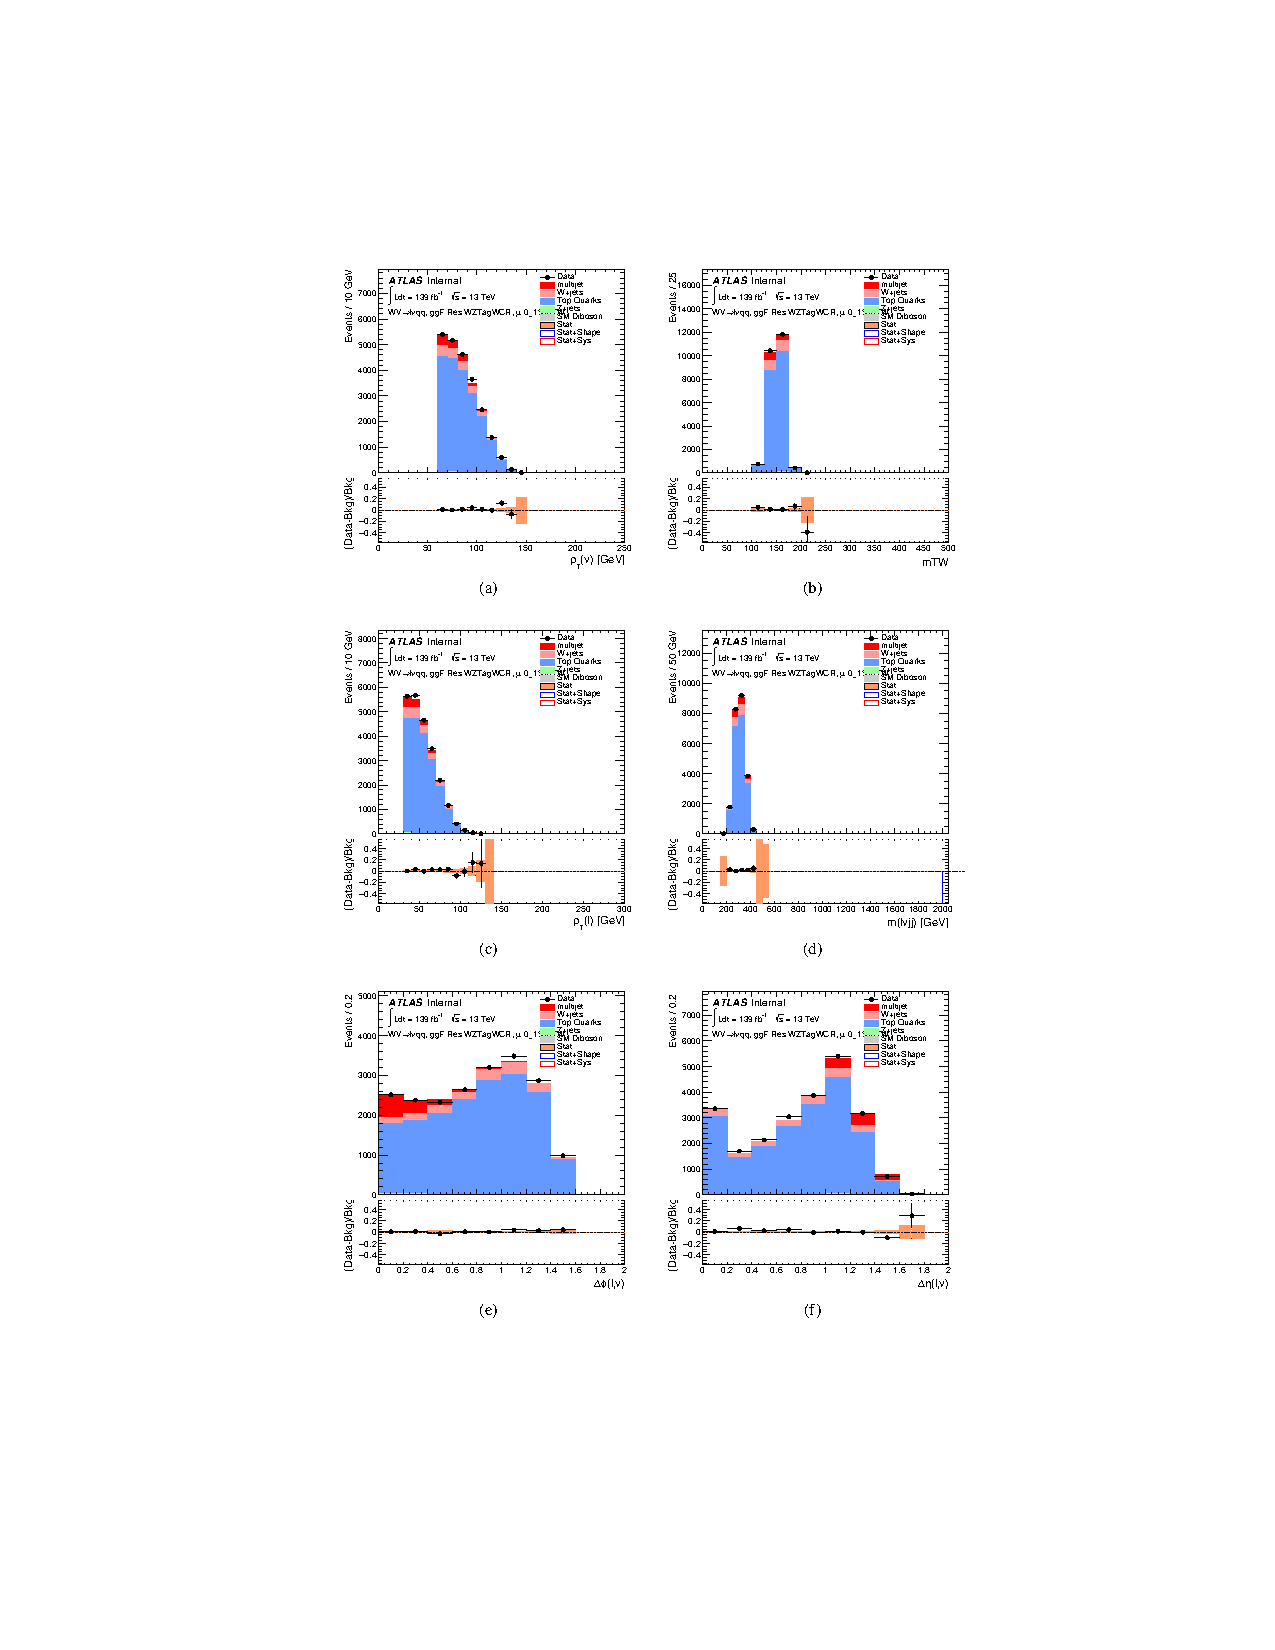
\includegraphics[width=\hsize , height=\textheight , keepaspectratio]{figures/Analysis/multijet/mj_muon_wz_tag.pdf}
      \caption{Postfit Data/MC comparison of distributions of $E_{T}^{miss}$, $m_{T}^{W}$, lepton and neutrino $p_{T}$, $m_{\ell \nu jj}$, lepton-$\nu$ angular distance in the $WZ$ untag muon channel. The MJ template is obtained from the pre-MJ-fit.} 
  \label{fig:multijet_met_muon_wz_untag}
\end{figure} 
\FloatBarrier



\begin{figure}[h!]
  \centering
  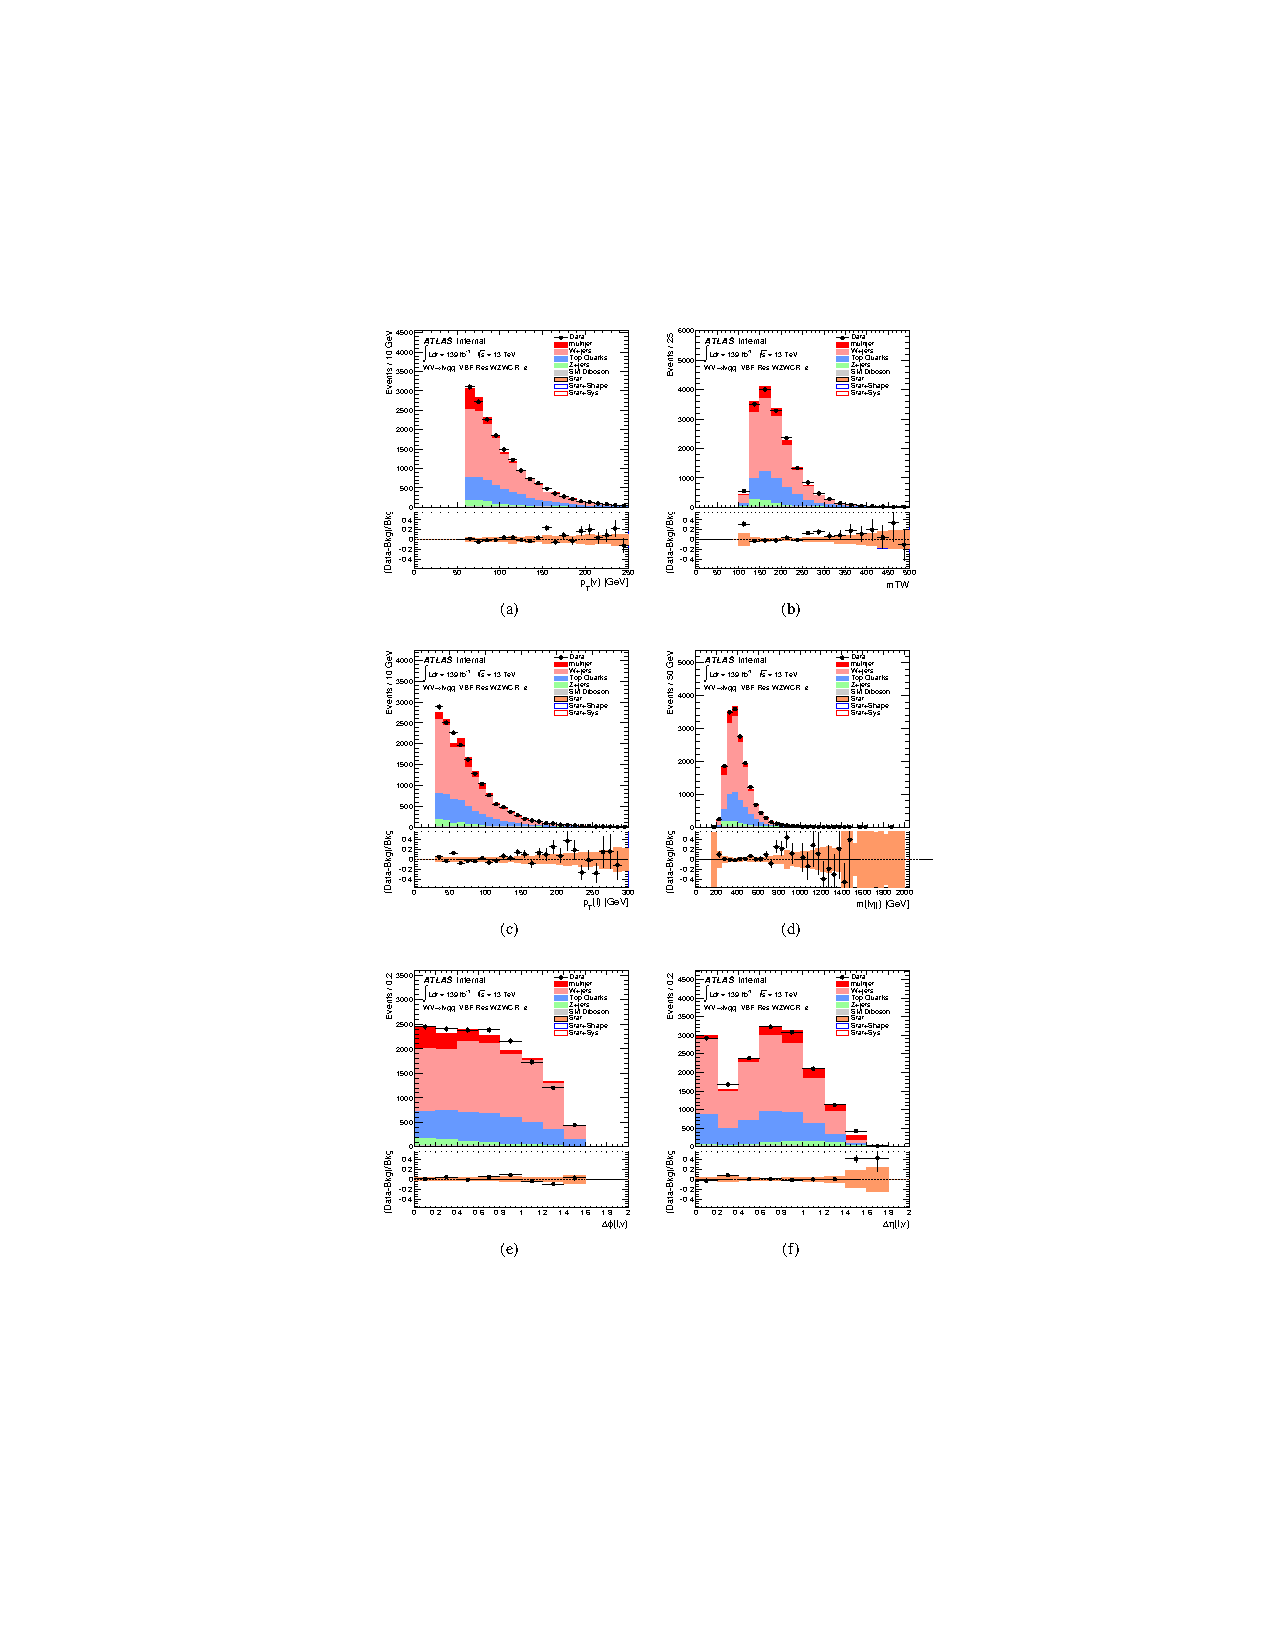
\includegraphics[width=\hsize , height=\textheight , keepaspectratio]{figures/Analysis/multijet/mj_elec_vbf_ww.pdf}
      \caption{Postfit Data/MC comparison of distributions of $E_{T}^{miss}$, $m_{T}^{W}$, lepton and neutrino $p_{T}$, $m_{\ell \nu jj}$, lepton-$\nu$ angular distance in the VBF $WW$ electron channel. The MJ template is obtained from the pre-MJ-fit.} 
  \label{fig:multijet_met_elec_ww_vbf}
\end{figure} 
\FloatBarrier


\begin{figure}[h!]
  \centering
  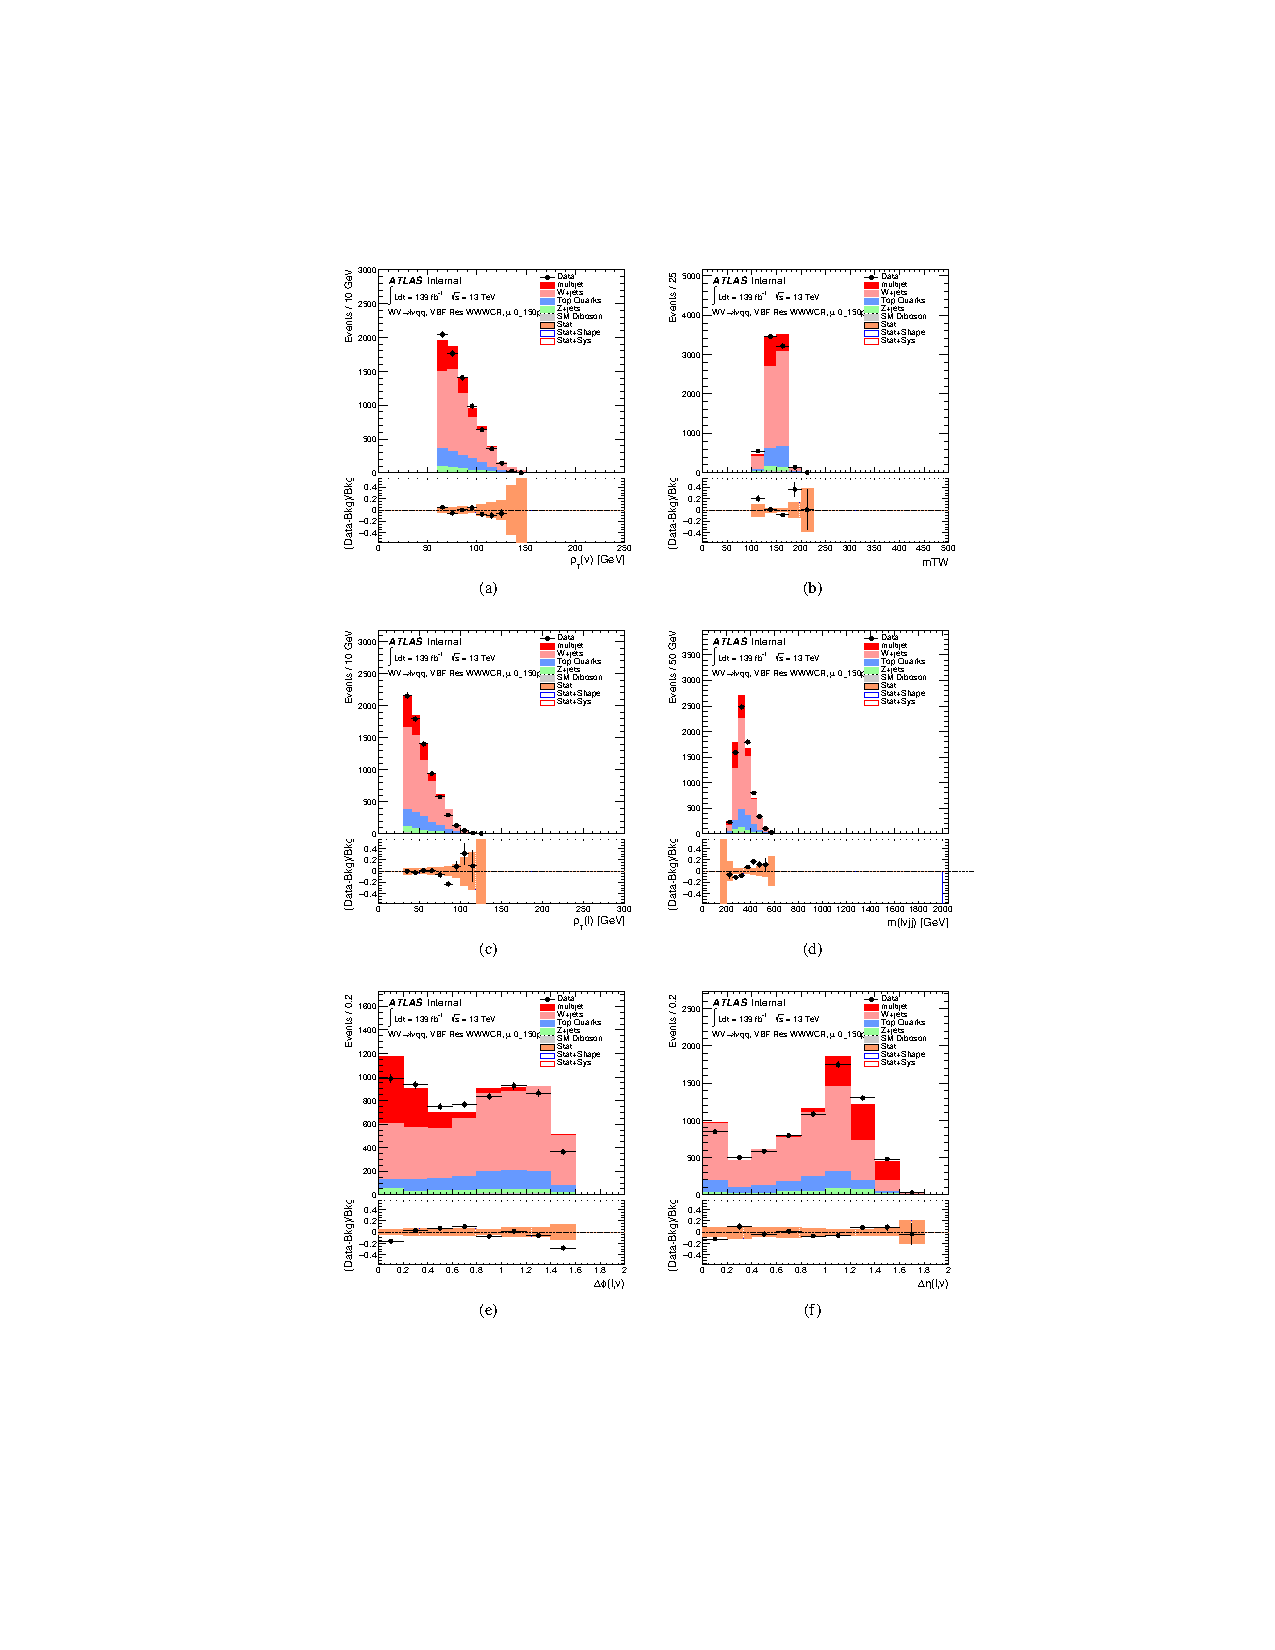
\includegraphics[width=\hsize , height=\textheight , keepaspectratio]{figures/Analysis/multijet/mj_muon_vbf_ww.pdf}
      \caption{Postfit Data/MC comparison of distributions of $E_{T}^{miss}$, $m_{T}^{W}$, lepton and neutrino $p_{T}$, $m_{\ell \nu jj}$, lepton-$\nu$ angular distance in the VBF $WW$ muon channel. The MJ template is obtained from the pre-MJ-fit.} 
  \label{fig:multijet_met_muon_ww_vbf}
\end{figure} 
\FloatBarrier


\begin{figure}[h!]
  \centering
  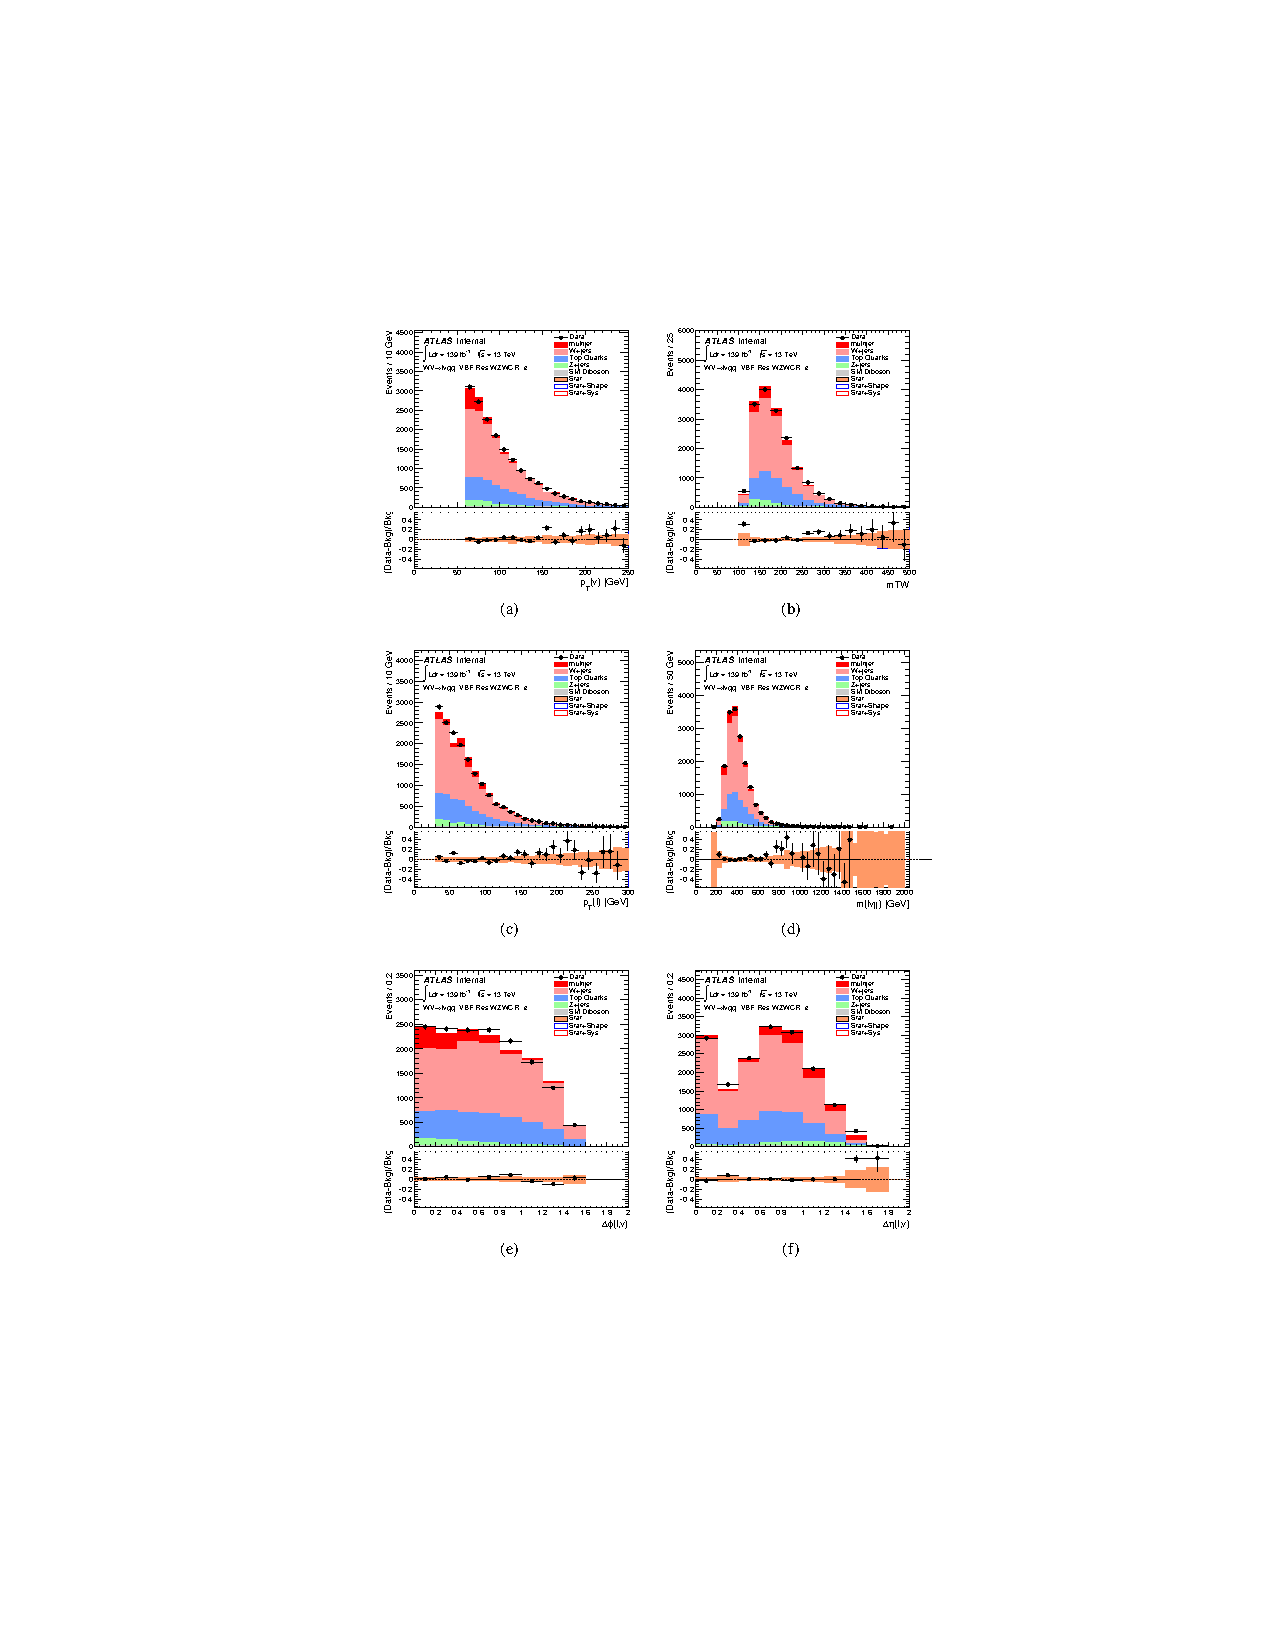
\includegraphics[width=\hsize , height=\textheight , keepaspectratio]{figures/Analysis/multijet/mj_elec_vbf_wz.pdf}
      \caption{Postfit Data/MC comparison of distributions of $E_{T}^{miss}$, $m_{T}^{W}$, lepton and neutrino $p_{T}$, $m_{\ell \nu jj}$, lepton-$\nu$ angular distance in the VBF $WZ$ electron channel. The MJ template is obtained from the pre-MJ-fit.} 
  \label{fig:multijet_met_elec_wz_vbf}
\end{figure} 
\FloatBarrier


\begin{figure}[h!]
  \centering
  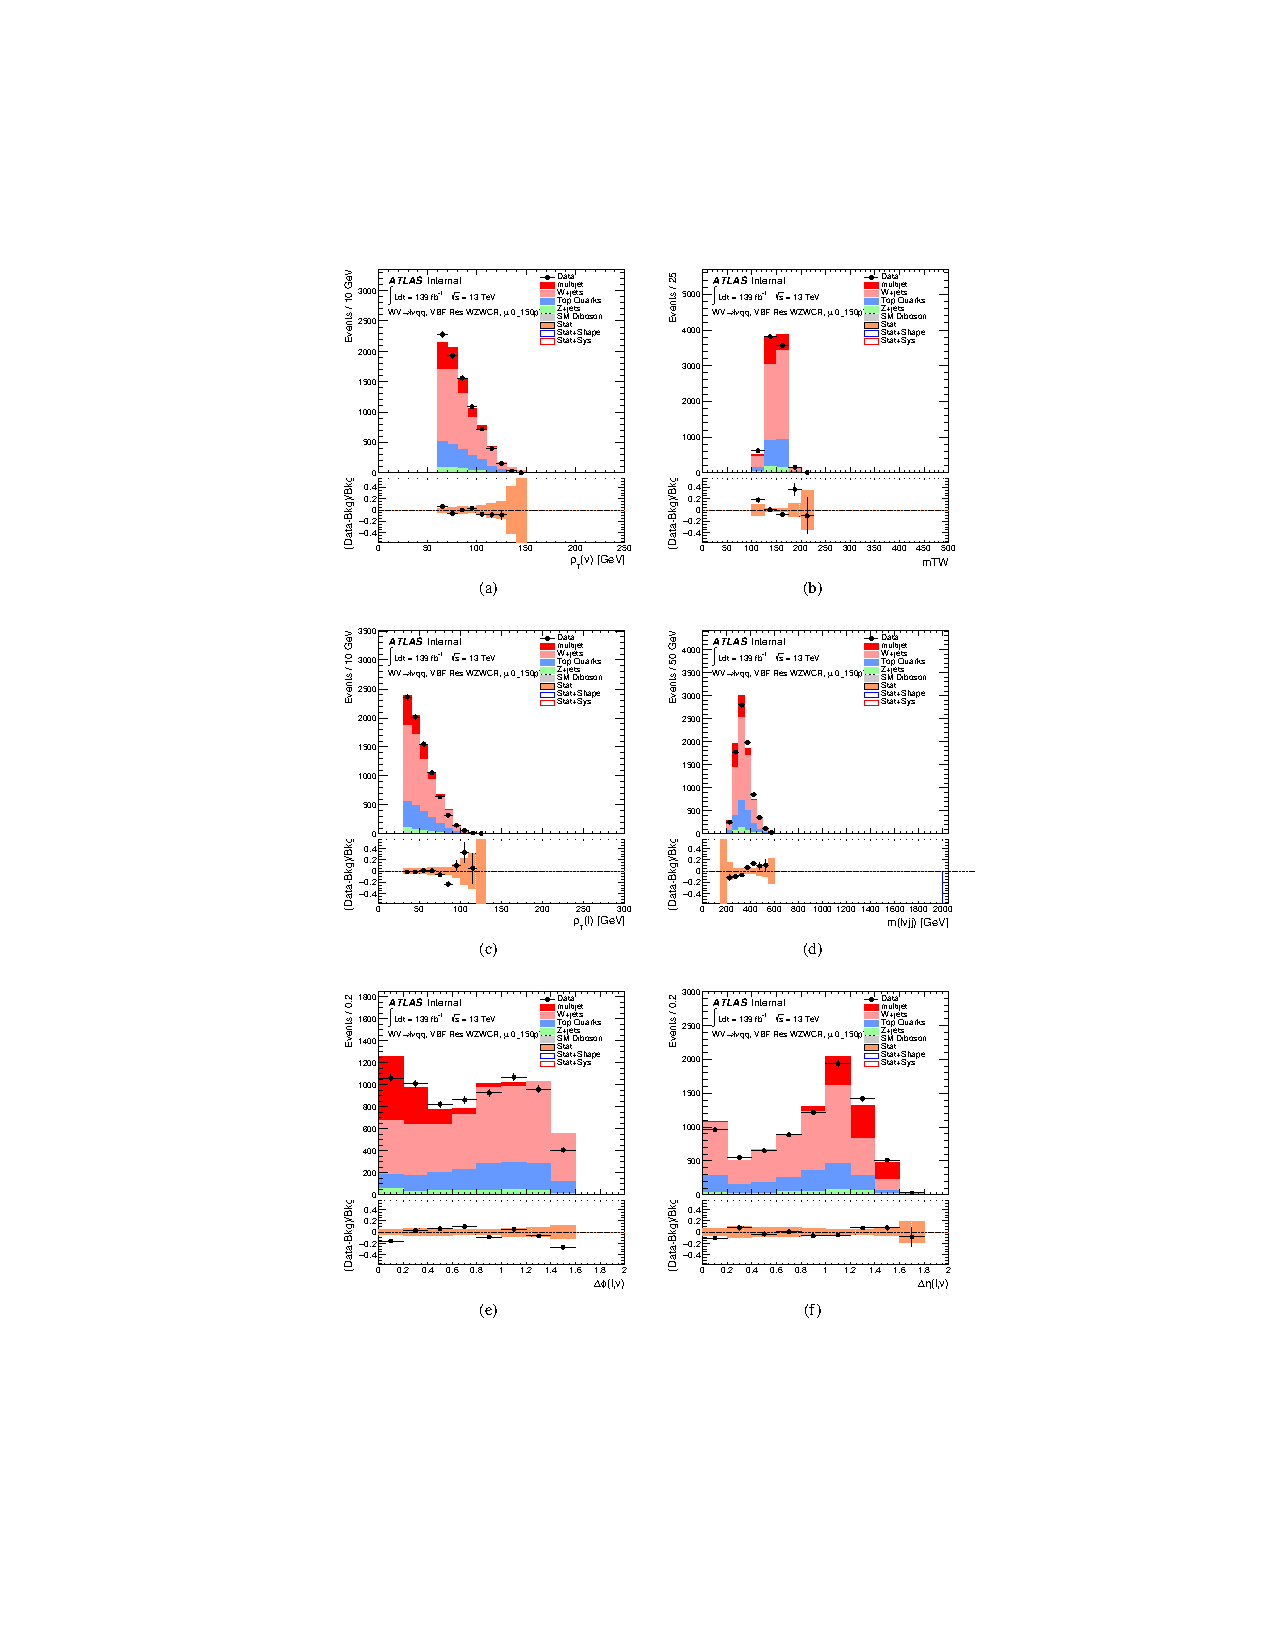
\includegraphics[width=\hsize , height=\textheight , keepaspectratio]{figures/Analysis/multijet/mj_muon_vbf_wz.pdf}
      \caption{Postfit Data/MC comparison of distributions of $E_{T}^{miss}$, $m_{T}^{W}$, lepton and neutrino $p_{T}$, $m_{\ell \nu jj}$, lepton-$\nu$ angular distance in the VBF $WZ$ muon channel. The MJ template is obtained from the pre-MJ-fit.} 
  \label{fig:multijet_met_muon_wz_vbf}
\end{figure} 
\FloatBarrier


\begin{table}[ht]
    \centering
     \Large{Full Run 2}\\
     \large{ggF Res WWWCR \\ }
     \begin{tabular}{|c|c|c|c|c|}
      \hline
     Sample    & Yield   & R.U.    & SF    \\ \hline
     Top\&W    & $645040\pm 1971.68$  & 0.31\%  & 0.998  \\ \hline
     Z\&VV     & $24075.9$ & \multicolumn{2}{c|}{fixed} \\ \hline
     MJ\_el    & $24156.3\pm 1224.62$  & 5.06\%  &3.973   \\ \hline
     MJ\_mu    & $35528.5\pm 923.94$  & 2.60\%  &9.019   \\ \hline
     \end{tabular}\hfill%
     \\
     \large{ggF Res WZ01bWCR\\ }
     \begin{tabular}{|c|c|c|c|c|}
      \hline
     Sample    & Yield   & R.U.    & SF    \\ \hline
     Top\&W    & $644690\pm 1981.4$  & 0.31\%  & 0.997  \\ \hline
     Z\&VV     & $24075.9$ & \multicolumn{2}{c|}{fixed} \\ \hline
     MJ\_el    & $24366.5\pm 1232.69$  & 5.05\%  &3.874   \\ \hline
     MJ\_mu    & $35528.5\pm 921.27$  & 2.58\%  &8.746   \\ \hline
     \end{tabular}\hfill%
     \\
     \large{ggF Res WZ2bWCR\\ }
     \begin{tabular}{|c|c|c|c|c|}
      \hline
     Sample    & Yield   & R.U.    & SF    \\ \hline
     Top\&W    & $71236.5\pm 688.74$  & 0.97\%  & 1.031  \\ \hline
     Z\&VV     & $518.5$ & \multicolumn{2}{c|}{fixed} \\ \hline
     MJ\_el    & $595.63\pm 449.34$  & 75.44\%  &0.094   \\ \hline
     MJ\_mu    & $1196.9\pm 222.13$  & 18.56\%  &0.294   \\ \hline
     \end{tabular}\hfill%
     \\
     \large{VBF Res WWWCR\\ }
     \begin{tabular}{|c|c|c|c|c|}
      \hline
     Sample    & Yield   & R.U.    & SF    \\ \hline
     Top\&W    & $19032.3\pm 364.43$  & 1.91\%  & 0.928  \\ \hline
     Z\&VV     & $1091.63$ & \multicolumn{2}{c|}{fixed} \\ \hline
     MJ\_el    & $1425.73\pm 214.42$  & 15.03\%  &0.235   \\ \hline
     MJ\_mu    & $1281.36\pm 157.21$  & 11.83\%  &0.314   \\ \hline
     \end{tabular}\hfill%
     \\
     \large{VBF Res WZWCR\\ }
     \begin{tabular}{|c|c|c|c|c|}
      \hline
     Sample    & Yield   & R.U.    & SF    \\ \hline
     Top\&W    & $21341.8\pm 392.21$  & 1.84\%  & 0.942  \\ \hline
     Z\&VV     & $1111.75$ & \multicolumn{2}{c|}{fixed} \\ \hline
     MJ\_el    & $1413.76\pm 230.36$  & 16.29\%  &0.225   \\ \hline
     MJ\_mu    & $1281.36\pm 157.21$  & 12.27\%  &0.314   \\ \hline
     \end{tabular}\hfill%
     \\
\caption{\label{tab:template_validation_CR} Fit validation result in WCRs for 2015+16 data. 
The fit is done in various WCRs, in order to obtain the corresponding scale factors for MJ templates: ggF resolved WCR for the $WW\to lvqq$ selection, ggF resolved untagged WCR for the $WZ\to lvqq$ selection,  ggF resolved tagged WCR for the $WZ\to lvqq$ selection,  VBF resolved WCR for the $WW\to lvqq$ selection,and VBF resolved WCR for the $WZ\to lvqq$ selection. Post-fit event yields for electroweak processes and MJ contributions are shown. The SF column shows the corresponding normalization scale factors for electroweak processes from the fit.
R.U. stands for relative uncertainty.
}
\end{table}



\chapter{Systematic Uncertainties}

This section describes the sources of systematic uncertainties considered in this analysis. These uncertainties are divided into three categories: experimental uncertainties, background modeling uncertainties, and theoretical uncertainties on signal processes. In the statistical analysis each systematic uncertainty is treated as a nuisance parameter estimated on the $m_{VV}$ distribution.

\section{Experimental Systematics}
The uncertainty on the integrated luminosity of the dataset used is 1.7\% and a systematic in the final fit. This uncertainty was calculated using $x-y$ beam separation scans [ref P55]. 

An additional source of systematic uncertainity is assigned to the pileup modeling in MC samples. This ensures simulated detector response and particle reconstruction conditions are as similar as possible. The distribution of the average number of interactions per bunch crossing applied to simulation is called the $\mu$ profile. The pileup modeling uncertainty is accounted for by re-weighting simulated events so the average number of interactions per bunch crossing varies within its uncertainty due to systematics from vertex reconstruction [ref ATL-COM-SOFT-2015-119]. The associated re-weighting factors are propagated through the entire analysis chain to construct a systematic uncertainty on $m_{VV}$.

The single-lepton and $E_{T}^{miss}$ triggers used are not fully efficient, so scale factors are applied to simulation to more accurately model the data. These scale factors are given by the ratio of the distribution of offline objects before trigger selection and after trigger selection. The associated uncertainty on these scale factors are used in the final fit.

Uncertainties on small-R jet energy scale and resolution are measured in-situ by calculating the response between data and simulation. This analysis uses a reduced set of JES and JER uncertainties (totaling 30 and 8 systematics, respectively). These reduced sets of systematics are calculated using a principal component analysis, yield largely uncorrelated independent systematics. These uncertainties on JES and JER account for the dependence on $p_{T}$, $\eta$, $\mu$, flavor response and global sequential corrections. Systematic uncertainties associated with $b$-tagging are also considered. These systematics are evaluated as uncertainties on the scale factor which account for the difference in $b$-tagging efficiencies in data and MC, and the flavor dependence (between b, c, and light jets). 

The uncertainty on the $p_{T}$ scale of the large-R jets is determined by comparing the jet's $p_{T}^{calo}$ to $p_{T}^{track}$ in di-jet simulation and data. In addition to this uncertainties from tracking, modeling (Pythia vs Herwig), and statistical constraints are also calculated. The large-R jet $p_{T}$ resolution is given by smearing the jet $p_{T}$ with a Gaussian with a 2\% width.

The $W/Z$-tagging efficiency cannot be evaluated using the Rtrk method as the TCC algorithm uses track measurements to reconstruct jet substructure variables. In order to avoid this potential bias, the $W/Z$-tagging is estimated in data using a control sample and corrected by comparing it with simulation. The efficiency to $W/Z$-induced signal is estimated by a $t\bar{t}$ control sample, while the efficiency to single-$q/g$ background is estimated using a dijet sample. The effects of experimental and theoretical uncertainties on the efficiency scale factor are determined by taking the ratio of efficiencies in data and simulation. By taking this ratio the uncertainties not arising for jet mass and $D_{2}$ cancel. 

Lepton identification, reconstruction, isolation systematic uncertainties are determined by reconstructing the Z mass peak with a tag and probe method. The lepton energy and momentum scales are also measured with the Z mass peak. Additionally, the track-to-vertex association efficiency is used for muons.

As $E_{T}^{miss}$ is calculated using all the physics objects in the event, all those objects associated errors result in an uncertainty on $E_{T}^{miss}$. Additionally, the unassociated tracks used to construct $E_{T}^{miss}$ contribute to the uncertainty on $E_{T}^{miss}$. 


\section{Theory Systematics}
Theoretical uncertainties for signal and background processes arise from uncertainties in the parameters used in Monte Carlo simulation. In particular for the $t\bar{t}$, $W/Z$+jets, diboson backgrounds and signal samples, the QCD scale, PDF, generator and hadronization uncertainties were evaluated. To assess the QCD scale uncertainty the renormalization and factorization scales were scaled up and down by a factor of two at the event generation stage of sample production. Uncertainties due to the choice of the parton distribution functions were evaluated by re-weighting samples from the nominal PDF to a set of error PDFs which account for the uncertainty of the fits used to produce the PDF set. In addition to this, samples are re-weighted to different PDF sets to account for the arbitrariness of the PDF choice. The difference between the $m_{WV}$ distributions using different event generators is assessed by comparing samples generated with different generators. Similarly, the uncertainty in hadronization models is accounted for by comparing samples created using different hadronization models (e.g. $t\bar{t}$ Powheg is compared to AMC@NLO, $W+jets$ compares Sherpa and MadGraph+Pythia samples). Figures \ref{fig:w_gen} - \ref{fig:ttbar_fsr_res} show the impact of these uncertainties on the $t\bar{t}$ and $W/Z$ + jets backgrounds. Additionally, contributions to the diboson background for the VBF analysis were found to be small and were accounted for by including a 5(10)\% systematic in the diboson normalization in the final fit.

The normalization of the $t\bar{t}$ and $W$+jets processes impact the multijet template shape. The impact of these normalizations was assessed by including a shape systematic on the multijet background from varying the $t\bar{t}$ and $W$+jets normalization factors. 

%fig:w_gen} - \ref{ttbar_fsr}


\begin{figure}[h!]
  \centering
  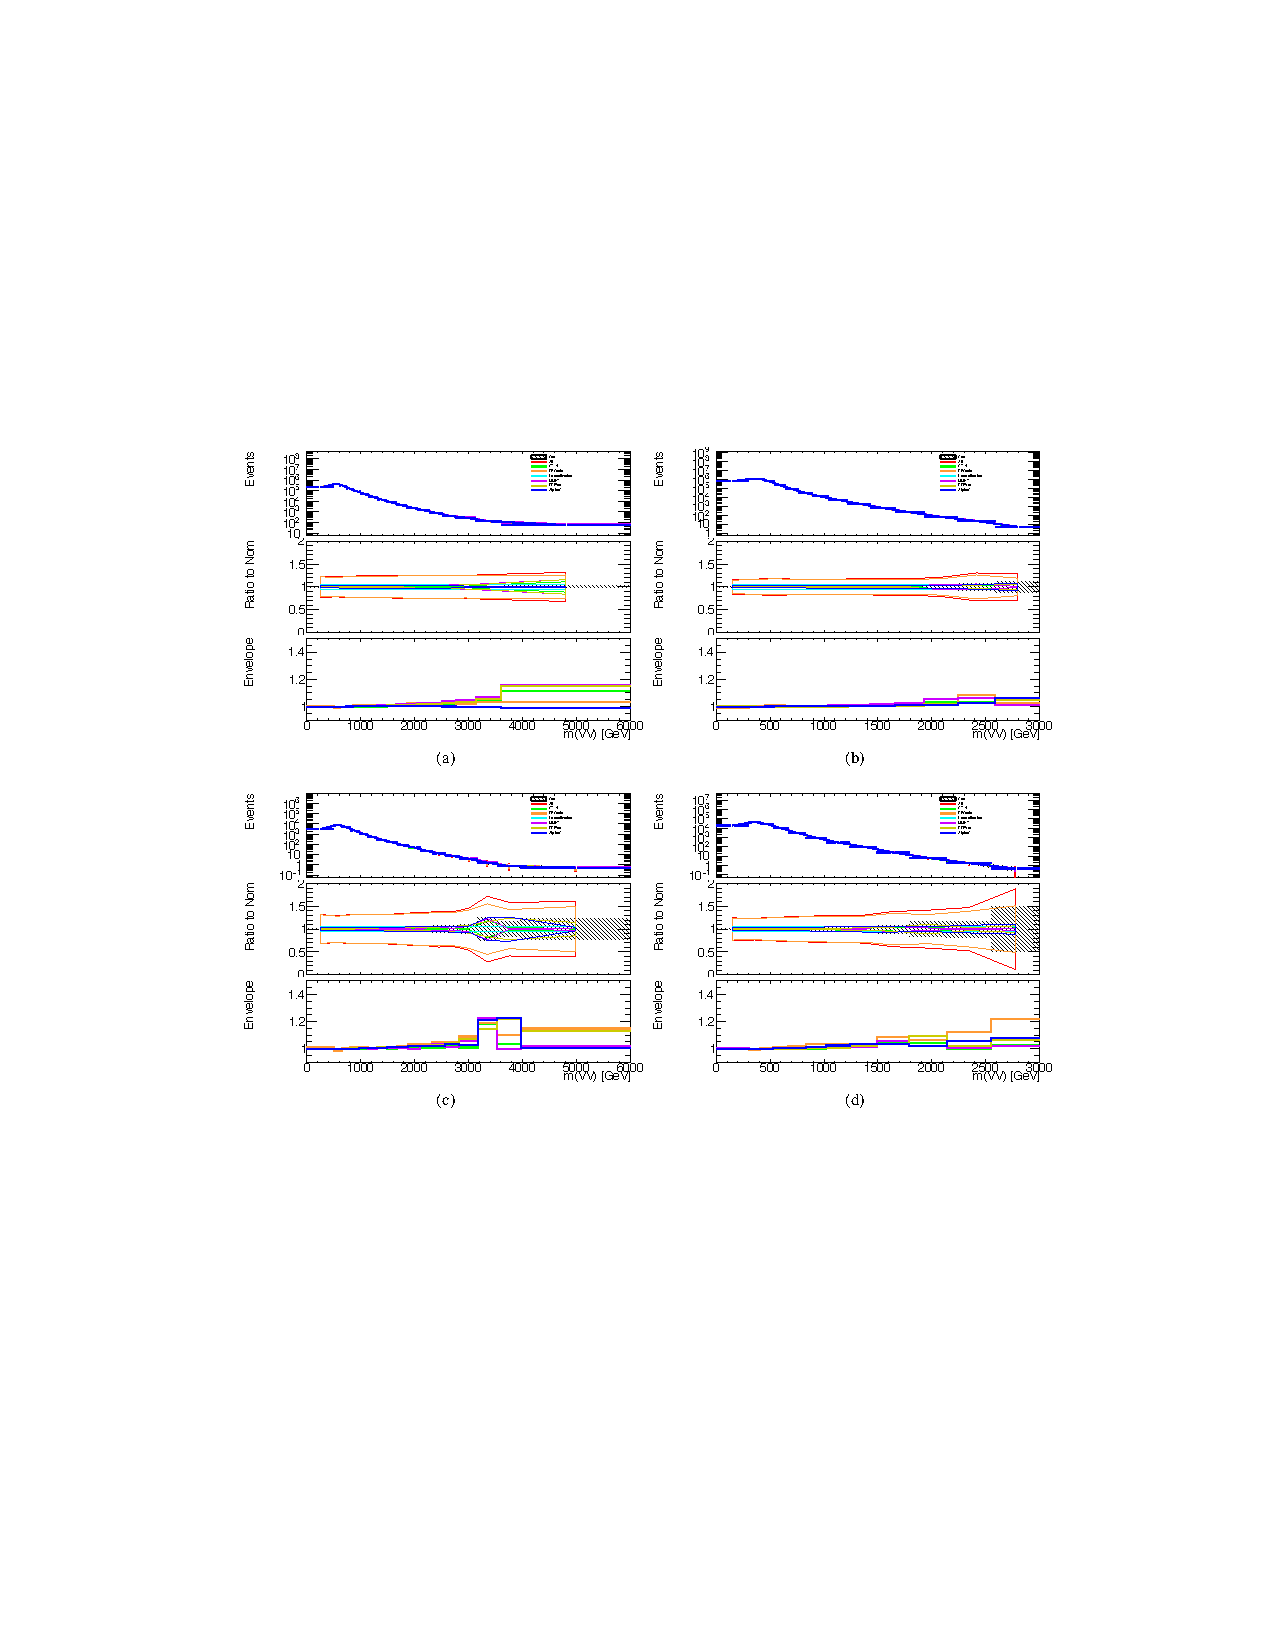
\includegraphics[width=\hsize]{figures/Analysis/modelingsysts/w_syst.pdf}
      \caption{The W/Z+jet systematics for the a) Merged ggF, b) Resolved ggF, c) Merged VBF, and d) Resolved VBF regions. The top subplot shows the nominal and variation distributions/bands, the middle shows the ratio of the two, and the final shows just the shape of the envelope (the final uncertainty).} 
  \label{fig:w_systs}
\end{figure} 
\FloatBarrier


\begin{figure}[h!]
  \centering
  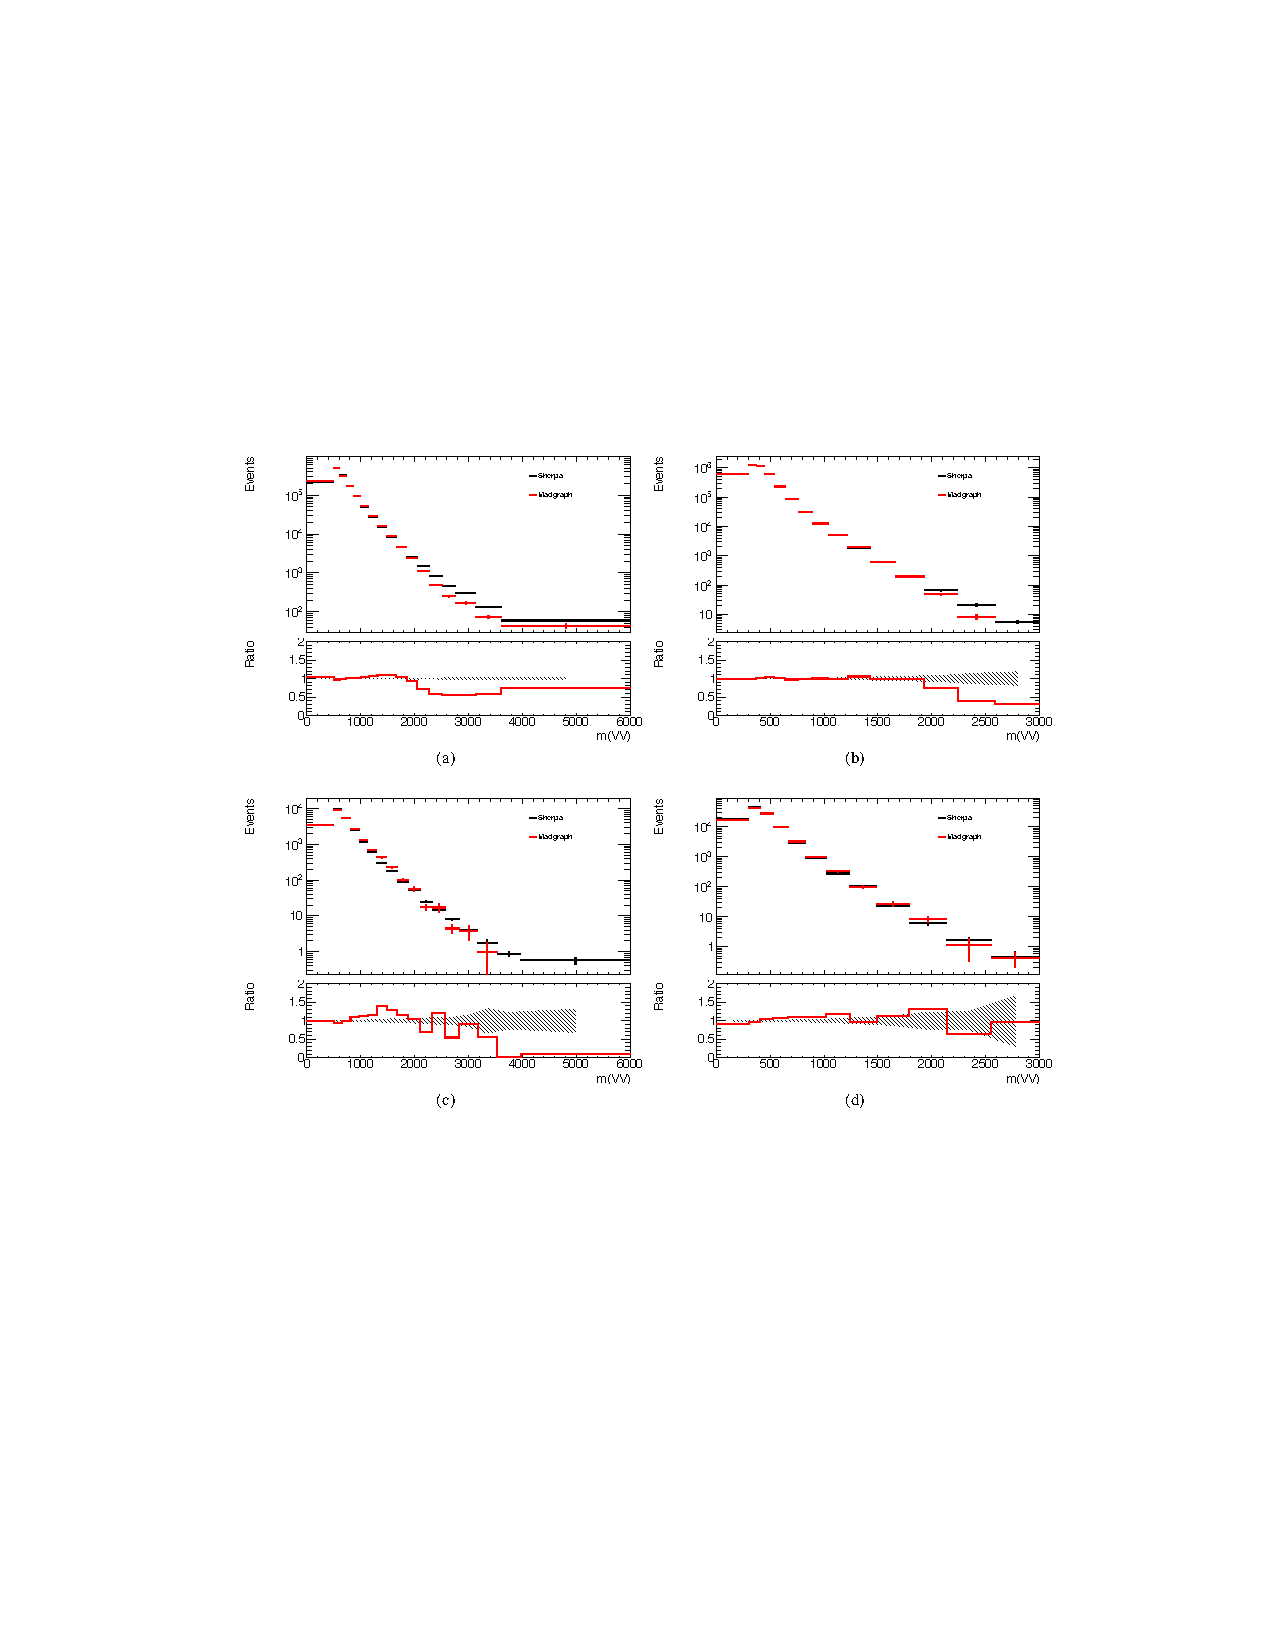
\includegraphics[width=\hsize]{figures/Analysis/modelingsysts/w_gen.pdf}
            \caption{The two-point generator comparison between Sherpa and MadGraph for the W/Z+jet samples in the a) Merged ggF, b) Resolved ggF, c) Merged VBF, and d) Resolved VBF regions. The normalization of the Madgraph sample is set to the Sherpa value to consider only shape effects. The bottom inlet shows the ratio of the two.} 
  \label{fig:w_gen}
\end{figure} 
\FloatBarrier



\begin{figure}[h!]
  \centering
  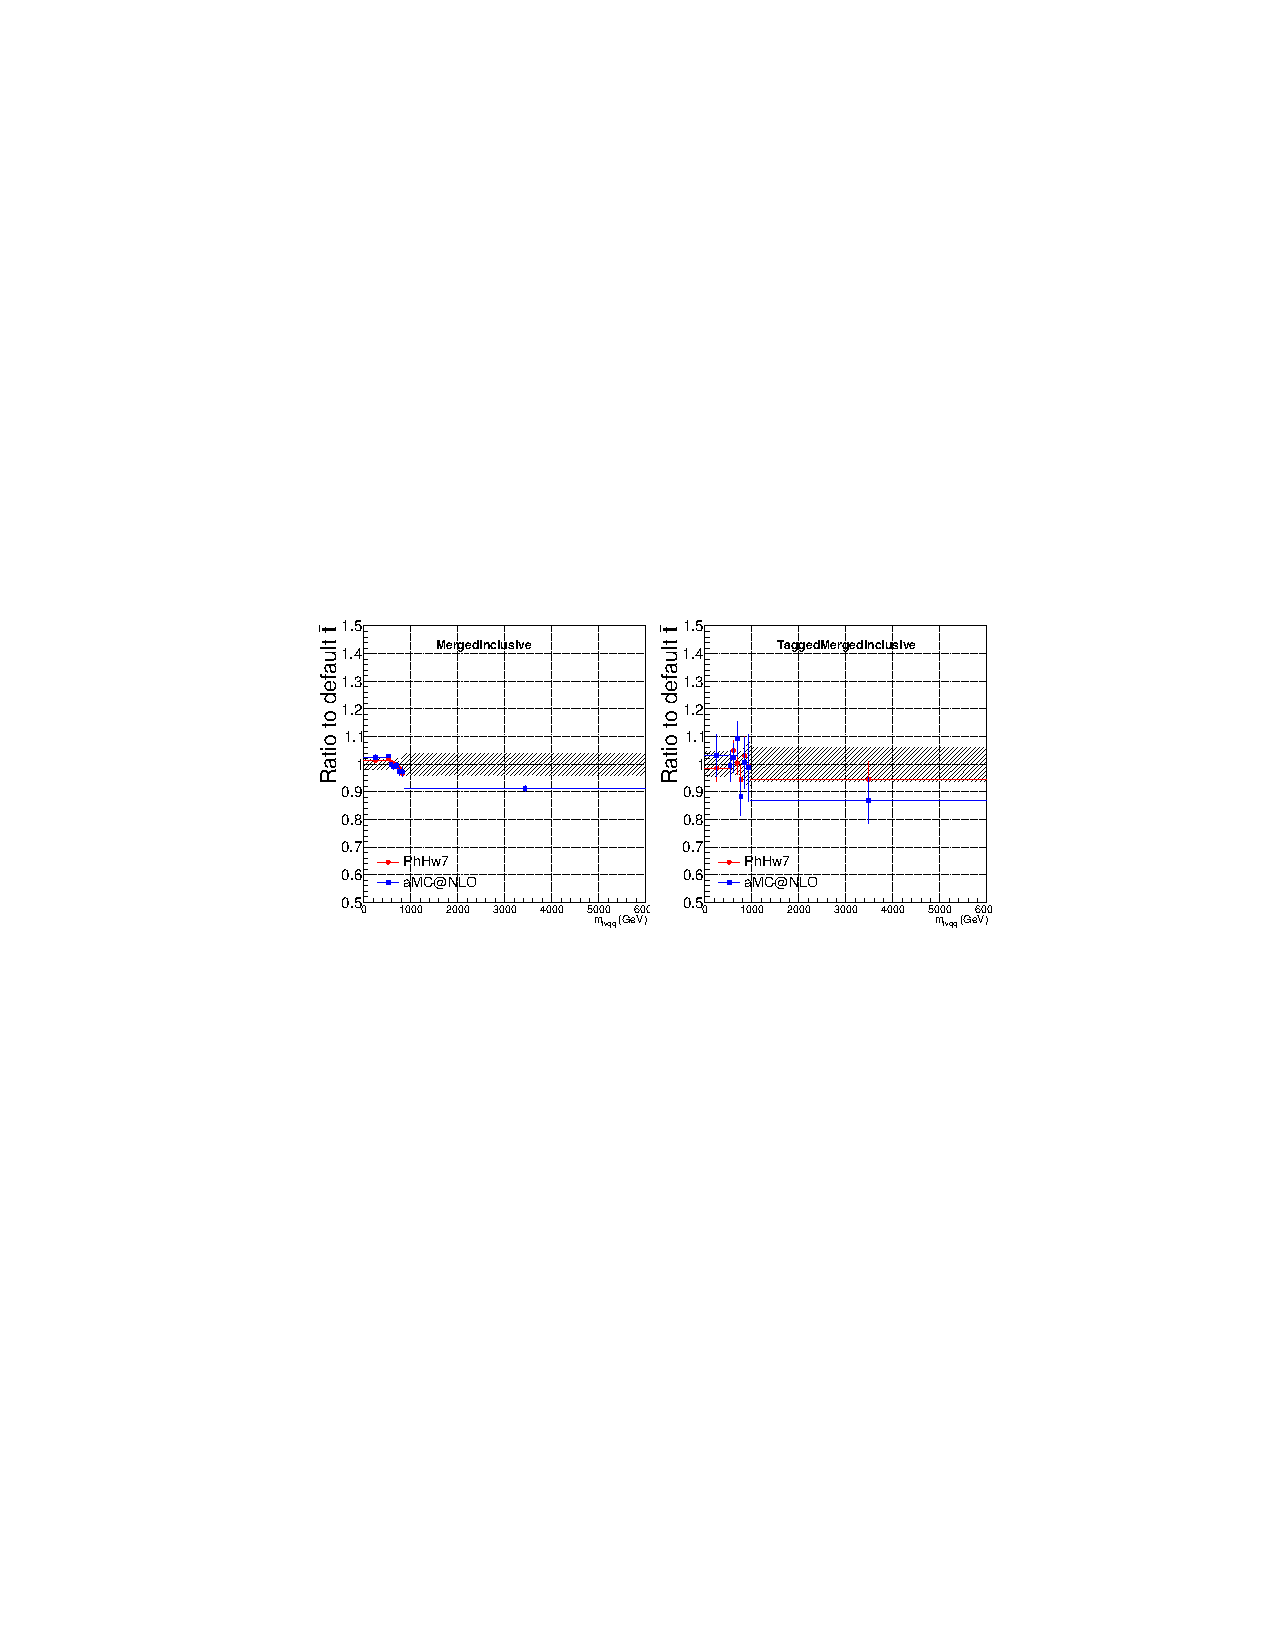
\includegraphics[width=\hsize]{figures/Analysis/modelingsysts/ttbar_gen_had_merg.pdf}
            \caption{Ratio between the variations of generator (red) and hadronization (blue) variations for the Merged regime for $t\bar{t}$ sample.} 
  \label{fig:ttbar_gen_merg}
\end{figure} 
\FloatBarrier


\begin{figure}[h!]
  \centering
  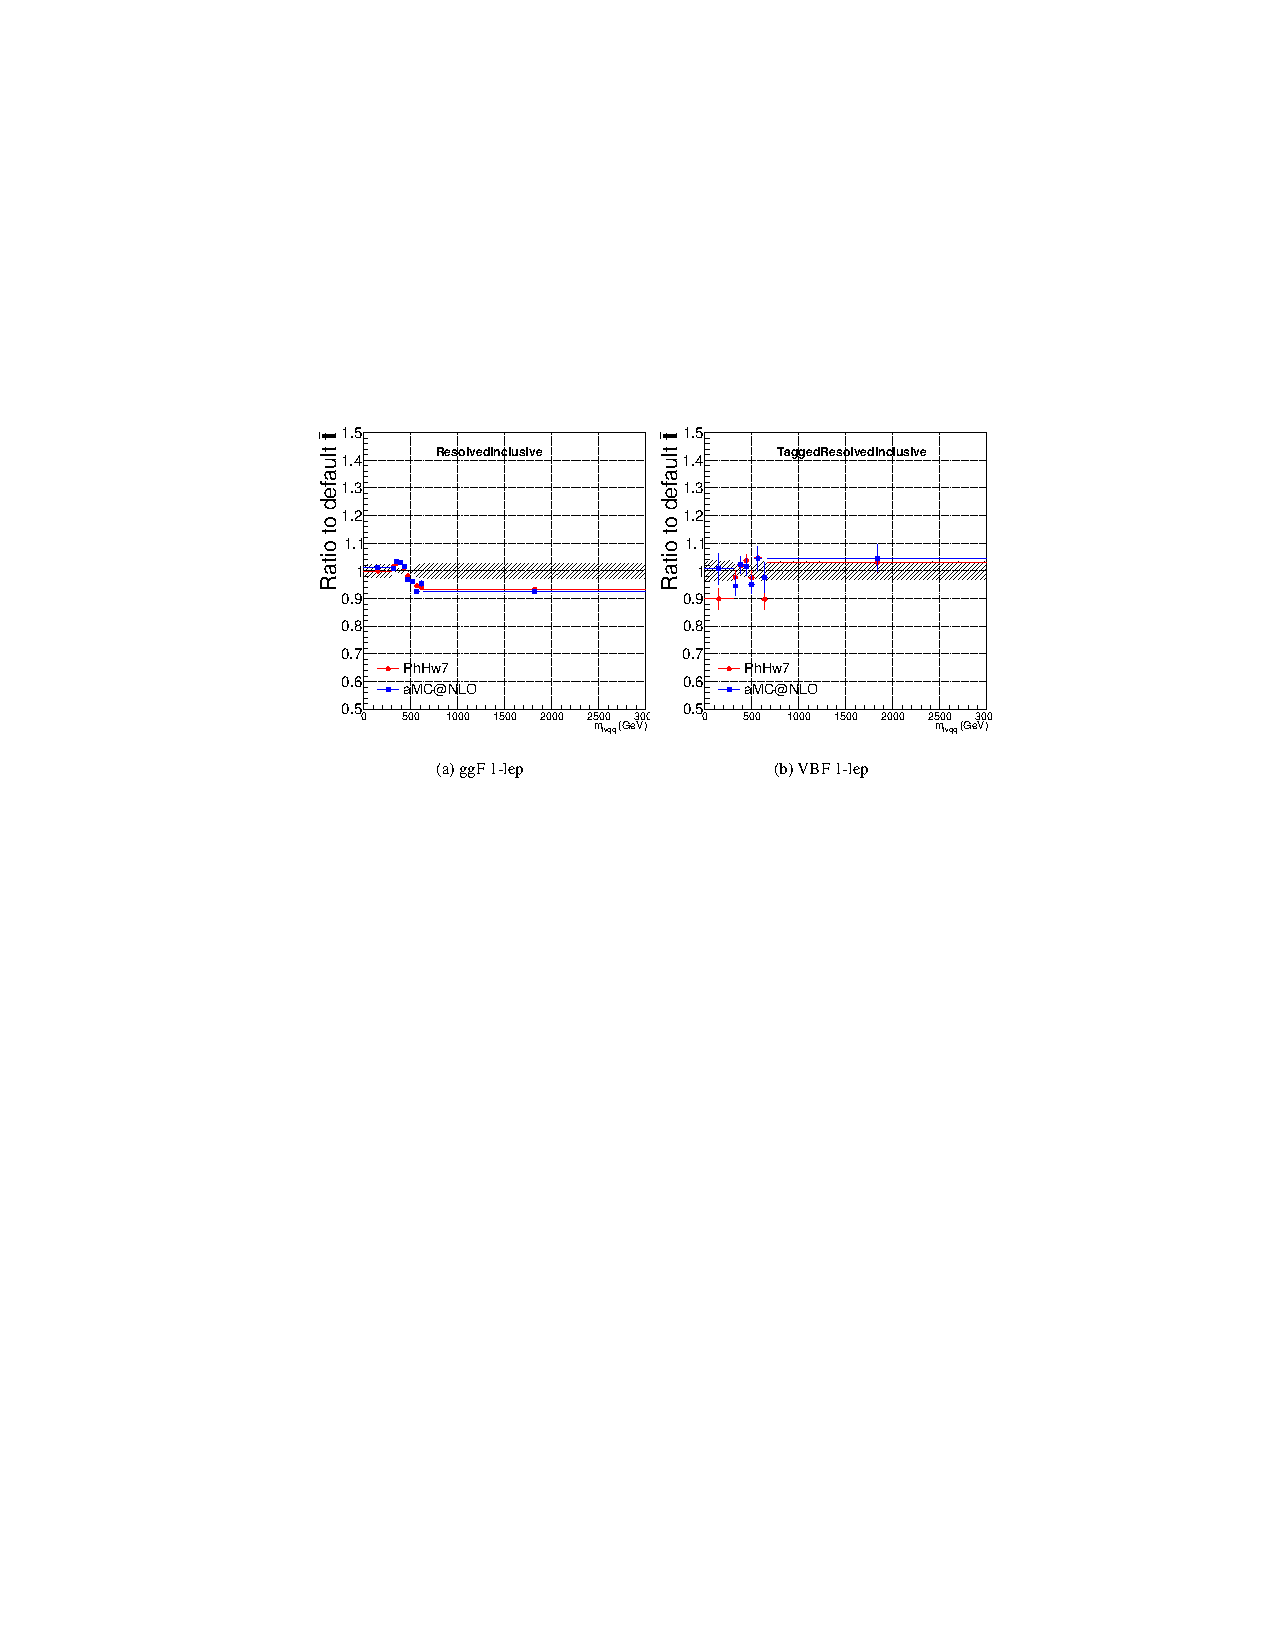
\includegraphics[width=\hsize]{figures/Analysis/modelingsysts/ttbar_gen_had_res.pdf}
            \caption{Ratio between the variations of generator (red) and hadronization (blue) variations for the Resolved regime for $t\bar{t}$ sample.} 
  \label{fig:ttbar_gen_res}
\end{figure} 
\FloatBarrier


\begin{figure}[h!]
  \centering
  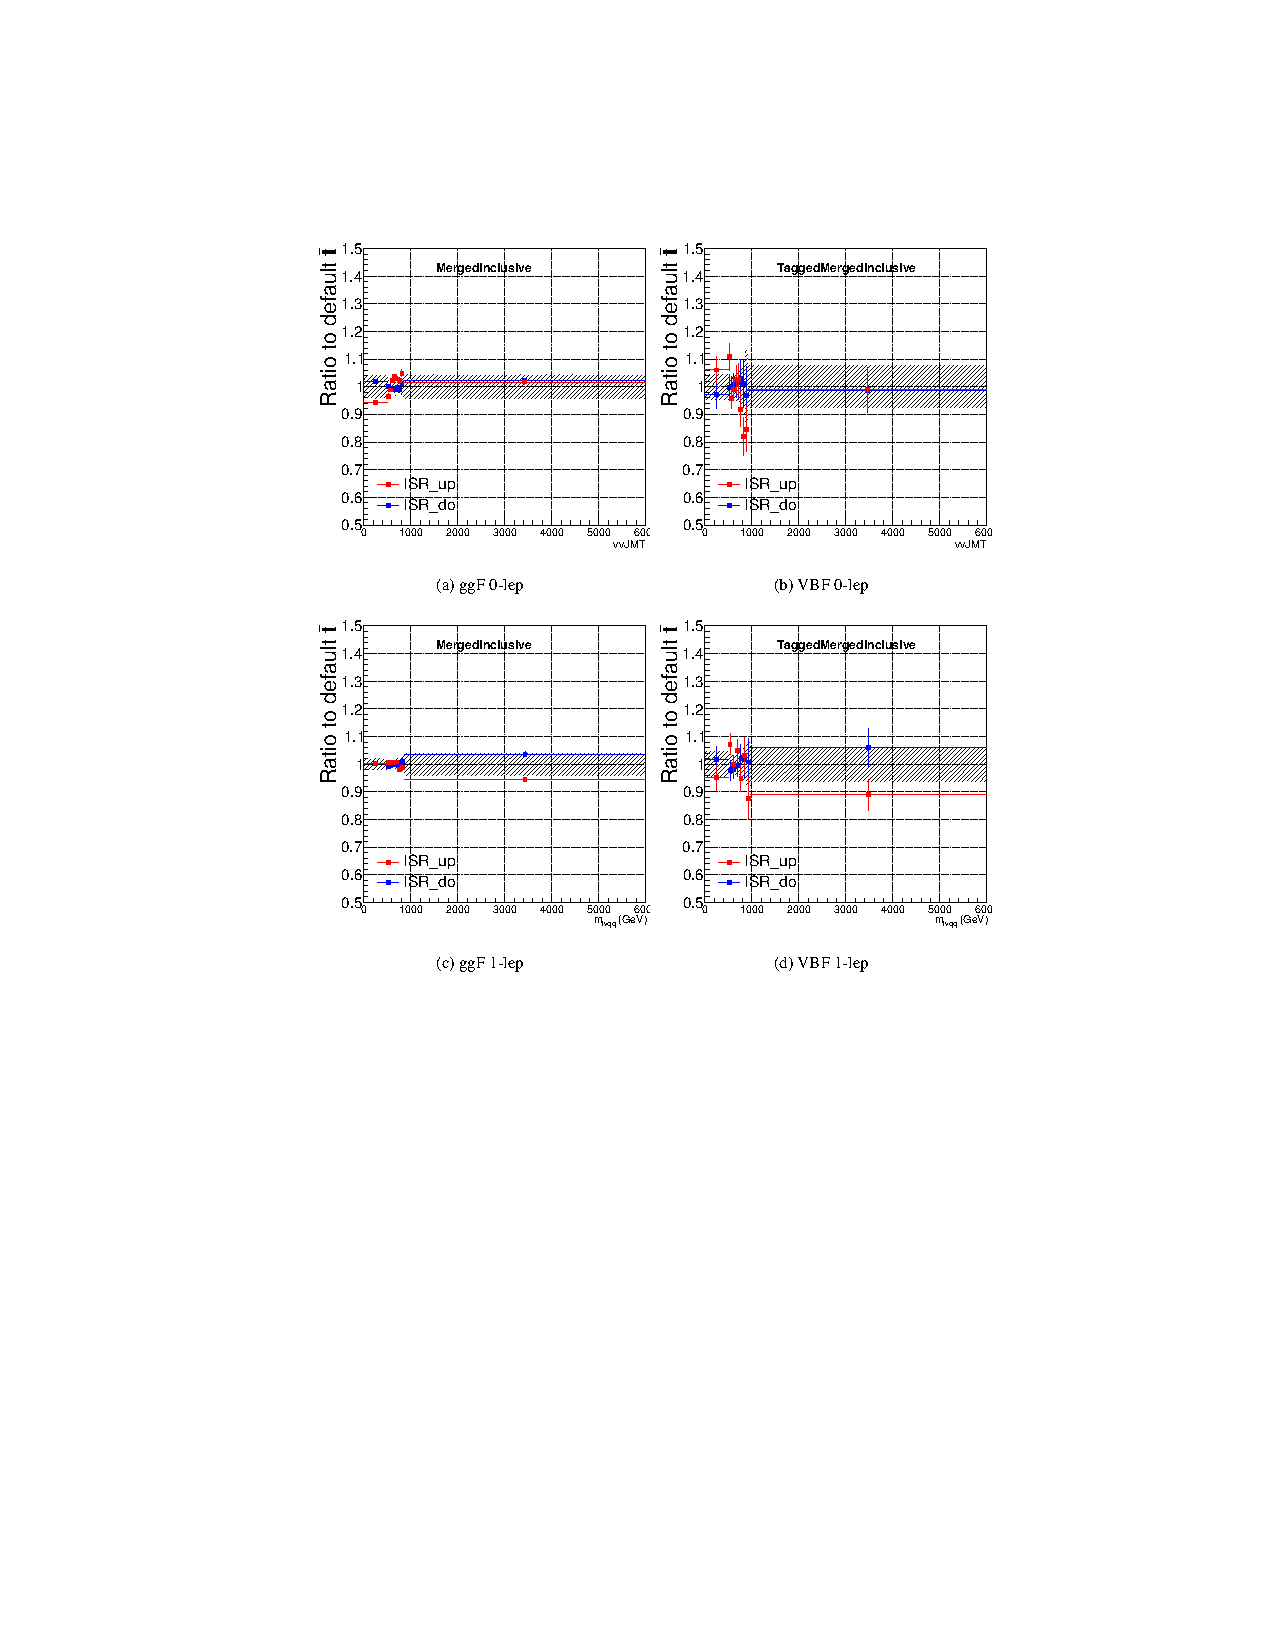
\includegraphics[width=\hsize]{figures/Analysis/modelingsysts/ttbar_isr_merg.pdf}
            \caption{Ratio between the variations of ISR up (red) and down (blue) variations for the Merged regime for $t\bar{t}$ sample.} 
  \label{fig:ttbar_isr_merg}
\end{figure} 
\FloatBarrier


\begin{figure}[h!]
  \centering
  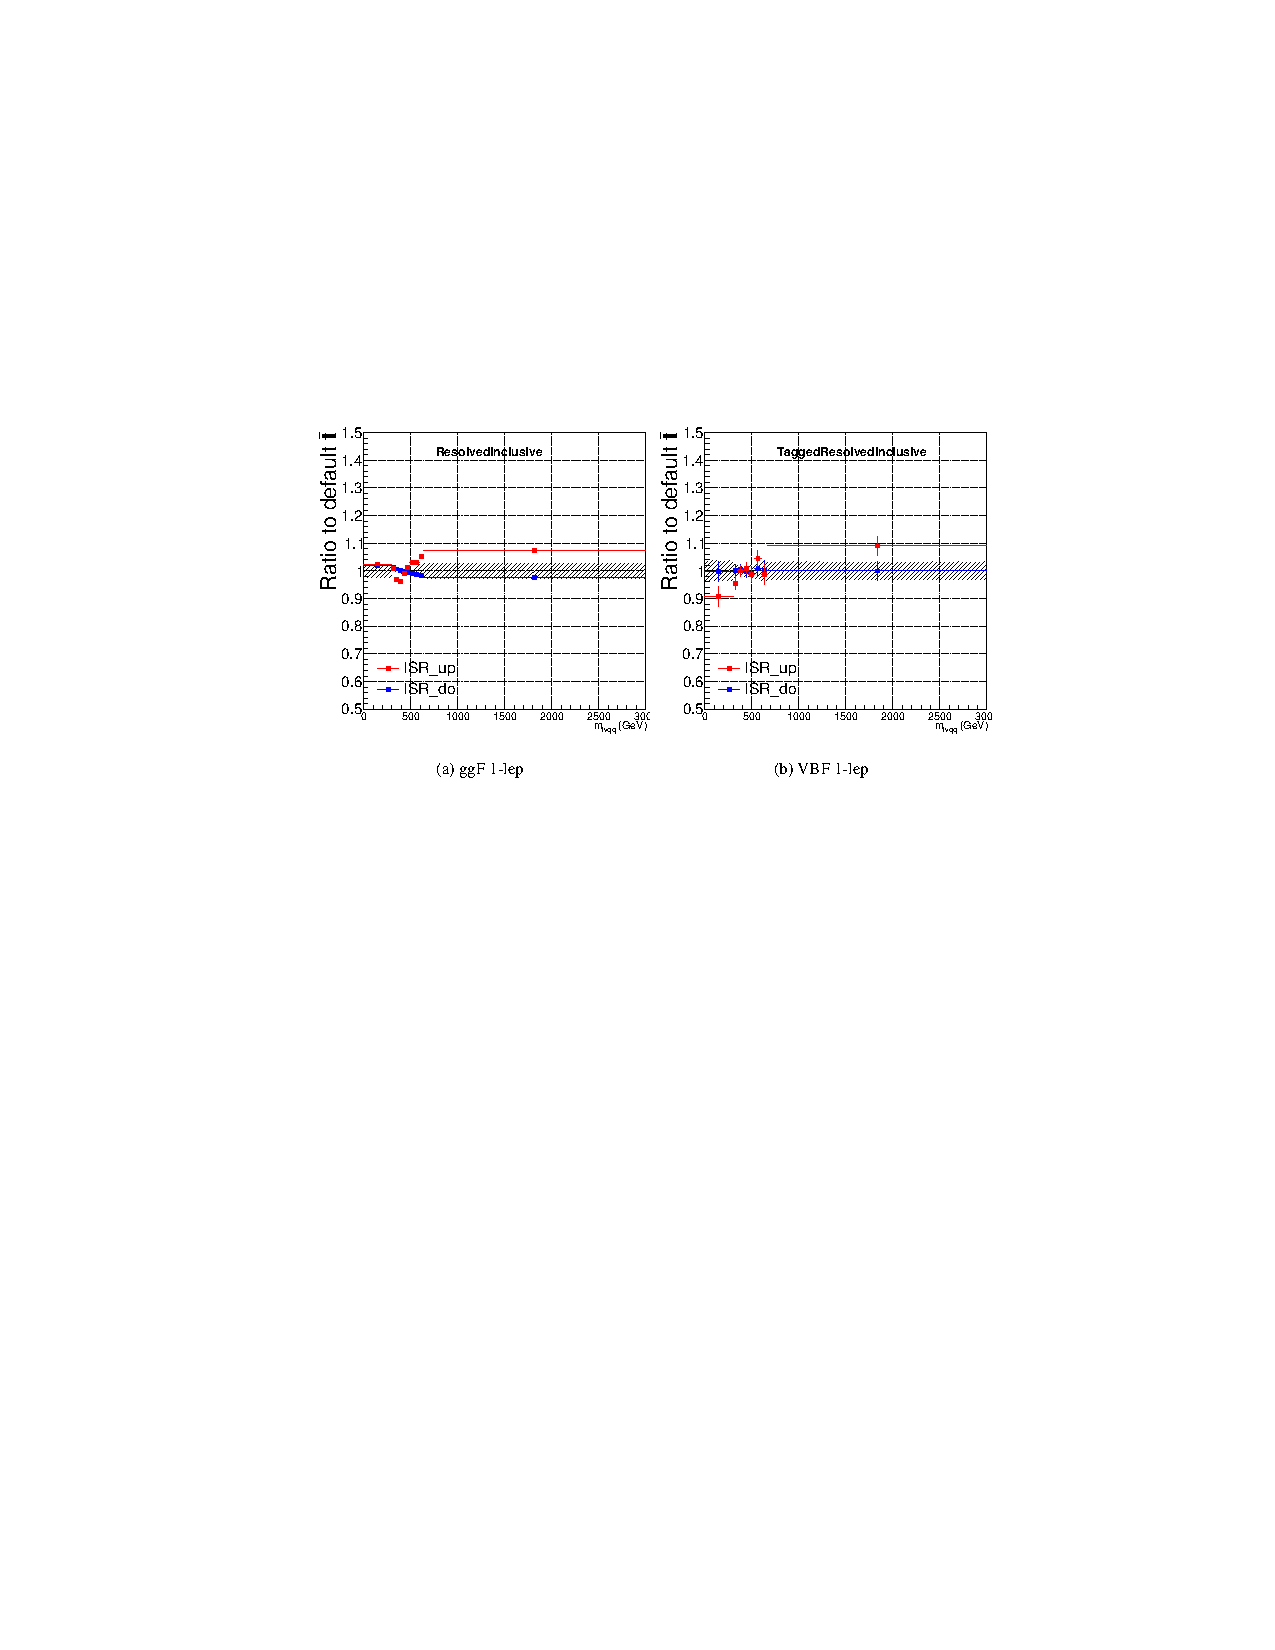
\includegraphics[width=\hsize]{figures/Analysis/modelingsysts/ttbar_isr_res.pdf}
            \caption{Ratio between the variations of ISR up (red) and down (blue) variations for the Resolved regime for $t\bar{t}$ sample.} 
  \label{fig:ttbar_isr_res}
\end{figure} 
\FloatBarrier


\begin{figure}[h!]
  \centering
  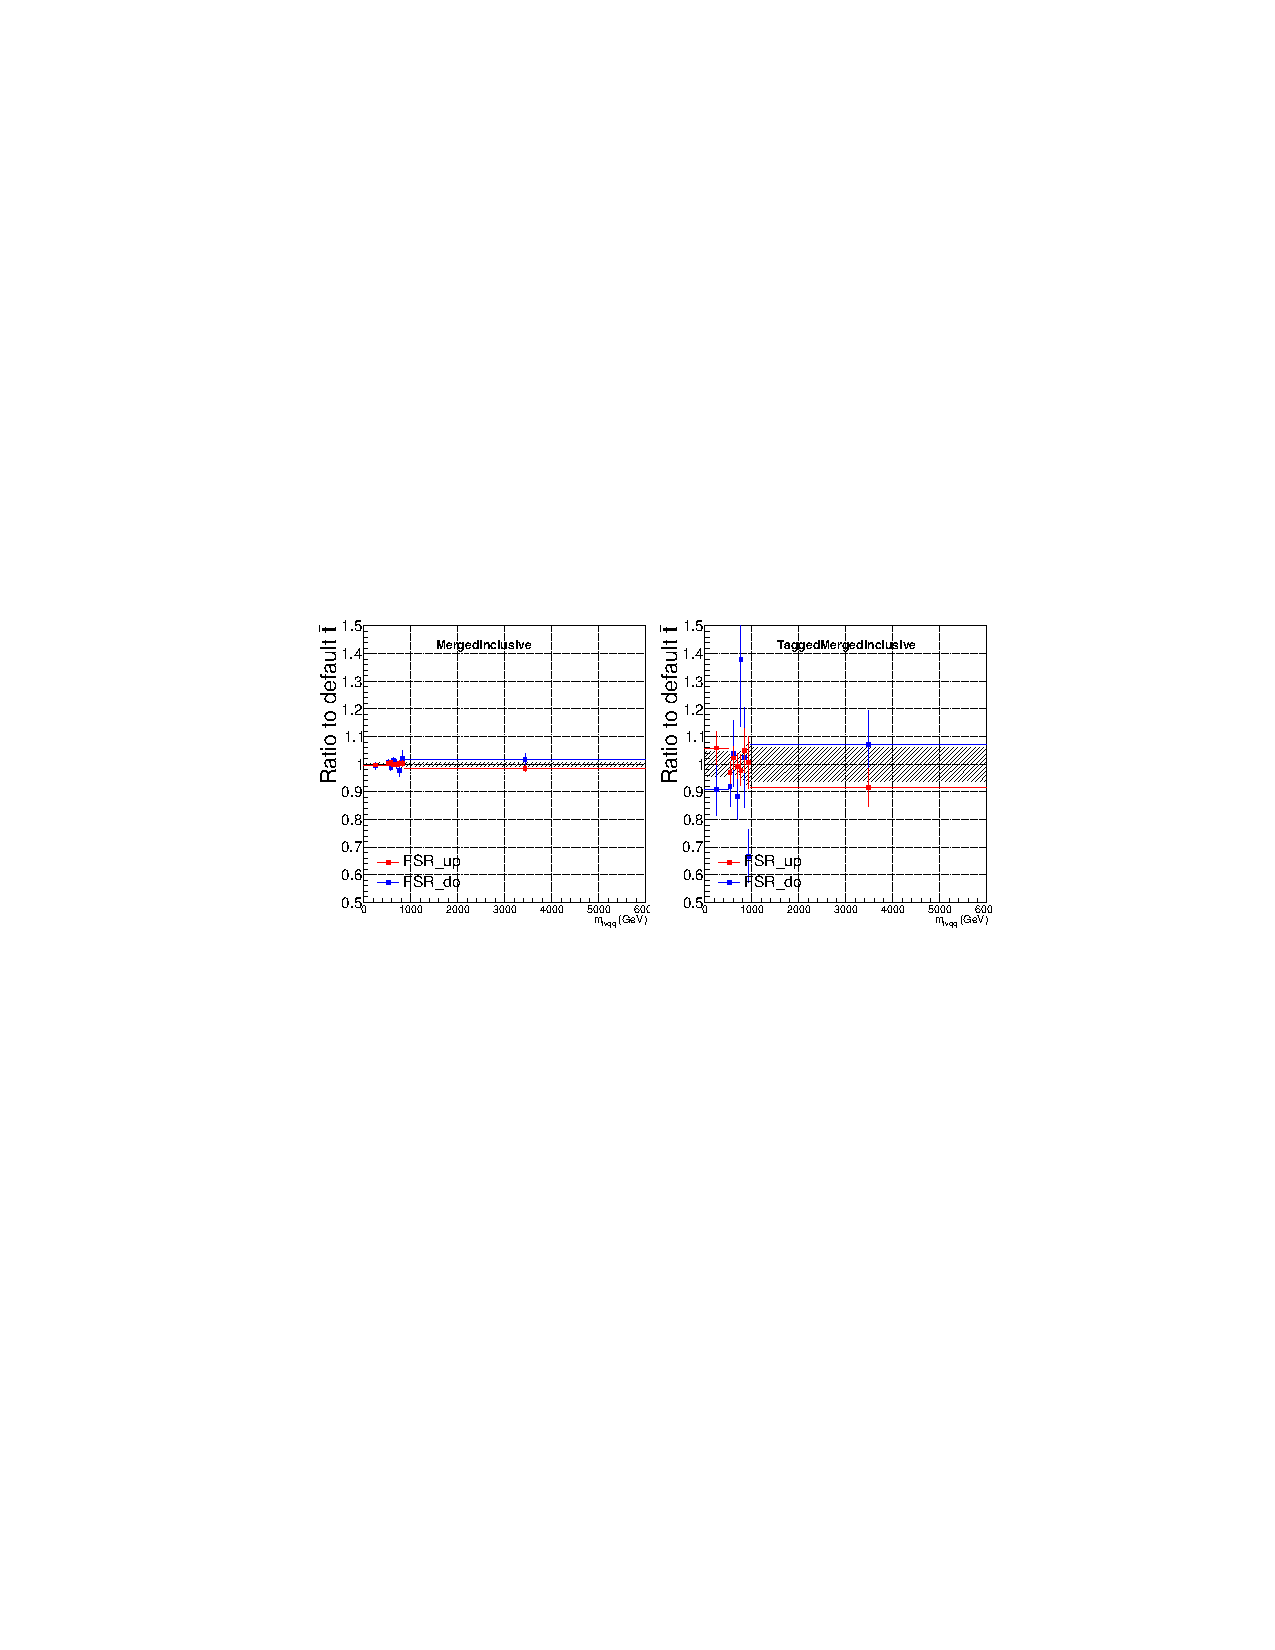
\includegraphics[width=\hsize]{figures/Analysis/modelingsysts/ttbar_fsr_merg.pdf}
            \caption{Ratio between the variations of FSR up (red) and down (blue) variations for the Merged regime for $t\bar{t}$ sample.} 
  \label{fig:ttbar_fsr_merg}
\end{figure} 
\FloatBarrier


\begin{figure}[h!]
  \centering
  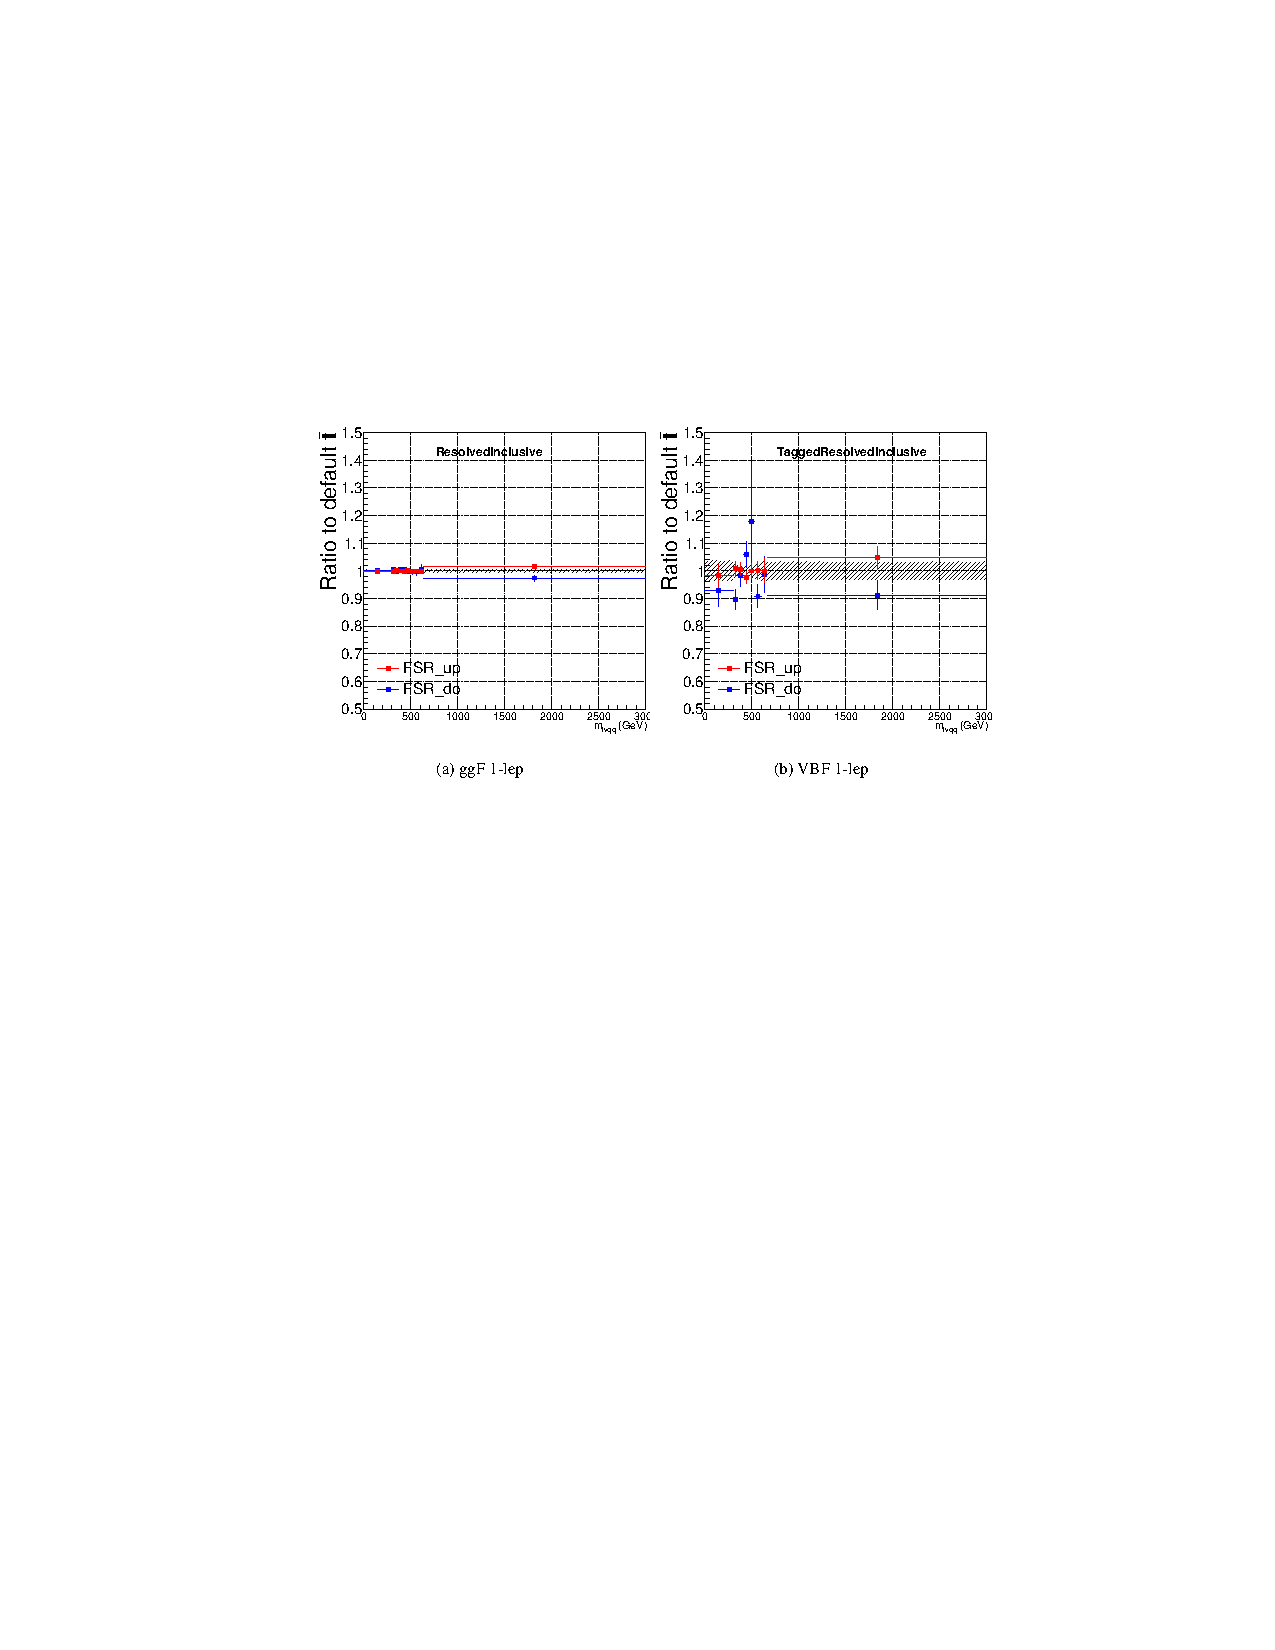
\includegraphics[width=\hsize]{figures/Analysis/modelingsysts/ttbar_fsr_res.pdf}
            \caption{Ratio between the variations of FSR up (red) and down (blue) variations for the Resolved regime for $t\bar{t}$ sample.} 
  \label{fig:ttbar_fsr_res}
\end{figure} 
\FloatBarrier

\chapter{Statistical Analysis}
To determine the compatibility of the data collected with the proposed resonances a statistical procedure based on a likelihood function is used. A discovery test is used to measure the compatibility of the observed data with the background only hypothesis. If the observed data is sufficiently incompatible with the background only hypothesis, this could indicate a discovery. In the absence of discovery, upper limits on the signal strength parameter, $\mu$, are assessed using the CLs method.

\section{Likelihood Function Definition}
The likelihood function is product of Poisson probabilities for all analysis bins and systematic constraints:

\begin{equation}
\mathcal{L}(\mu,\bm{\theta})= \prod_{c} \prod_{i} \frac{(\mu s_{ci}(\bm{\theta}) + b_{ci}(\bm{\theta}))^{n_{ci}}}{n_{ci}!} e^{-(\mu s_{ci}(\bm{\theta})+b_{ci}(\bm{\theta}))}\prod_{k}(\theta^{'}_{k}|\theta_{k})
\end{equation}

Here $c$ are the analysis channels considered and $i$ runs over all the $m_{\ell\nu qq}$ bins used in the fit. The signal strength parameter, $\mu$, multiplies the expected signal yield in each analysis bin, $s_{ci}$. The background content for channel $c$ and bin $i$ is given by $b_{ci}$ . The dependence of signal and background predictions on systematic uncertainties is described by the aforementioned set of nuisance parameters $\bm{\theta}$, which are parameterized by Gaussian or log-normal priors denoted here as $\theta_{k}$. Statistical uncertainties of the simulated bin contents are also included as systematic uncertainties. Most systematics are correlated among all the analysis regions and considered to be independent from each other. The validity of this assumption is checked by evaluating the covariance of nuisance parameters.  

\section{Fit Configuration}
The binning of $m_{\ell \nu qq}$ in signal regions for likelihood fit is determined by the statistical uncertainty of signal mass width. For each signal mass point, the signal mass resolution is given by the fitted Gaussian width of the $m_{\ell \nu qq}$. The fitted signal widths are then fit to a line to give a parameterized signal mass width, as shown in Figures \ref{fig:resolved_sigwidth} and \ref{fig:merged_sigwidth}. Bin widths are set first to this parameterized signal mass resolution. Then if the statistical uncertainty of the data or simulated background is more than 50\%, bins are merged until the statistical uncertainty is less than 50\%. All control regions contain only a single bin.

For this analysis, each signal model is fit in the Merged and Resolved channels for the relevant signal production mode simultaneously. The $W$+jets and $t\bar{t}$ normalizations are given by the best fit values in the overall fit and these fitted normalizations are then applied to those backgrounds in the SRs.

Systematics may be affected by low statistics, leading to unsmooth $m_{VV}$ distributions with unphysically large fluctuations. This can lead to artificial pulls and constraints in the fit. To remove such issues a multi-step smoothing procedure is applied to all systematic variation distributions in all regions. First, distributions are rebinned until the statistical error per bin is at least 5\%. Next all local extrema are identified. The bins around smallest extrema are iteratively merged until only four local extrema remain. Then distributions are rebinned so that statistical uncertainties in each bin are $< 5\%$.

For some systematics, up and down variations may be in the same direction with respect to the nominal distributions. This causes the variations to not cover the nominal choice, and the interpretation of the confidence interval is skewed as the nominal distribution should be bracketed by the up and down variations. This asymmetry may also lead to unconstrained systematics in the fit. To handle such asymmetric systematics, if the up and down variation for a given systematic are in the same direction for at least three $m_{VV}$ bins the variation is averaged for those bins. The averaging procedure replaces bin-by-bin the up and down variation bins by $b_{\pm}^{new}=b_{nom}\pm\frac{|b_{+}-b_{-}|}{2}$, where $b_{nom}$ is the nominal bin content and $b_{\pm}$ are the original up and down variation bin content. The same procedure is also applied to any variations where the integral of the difference between the up/down variation and the nominal distribution is twice that of the other down/up variation, further ensuring variations are symmetric around the nominal distribution.

Finally, systematics that have a negligible effect on the $m_{WV}$ distribution are not considered in the fit. Shape systematics where no bin in the variational distribution deviates more than $1\%$ from the nominal distribution (after normalizing all histograms to the nominal) are not included in the fit. Also, statistical bin uncertainties $< 1\%$ are ignored. 

\begin{figure}[h!]
  \centering
  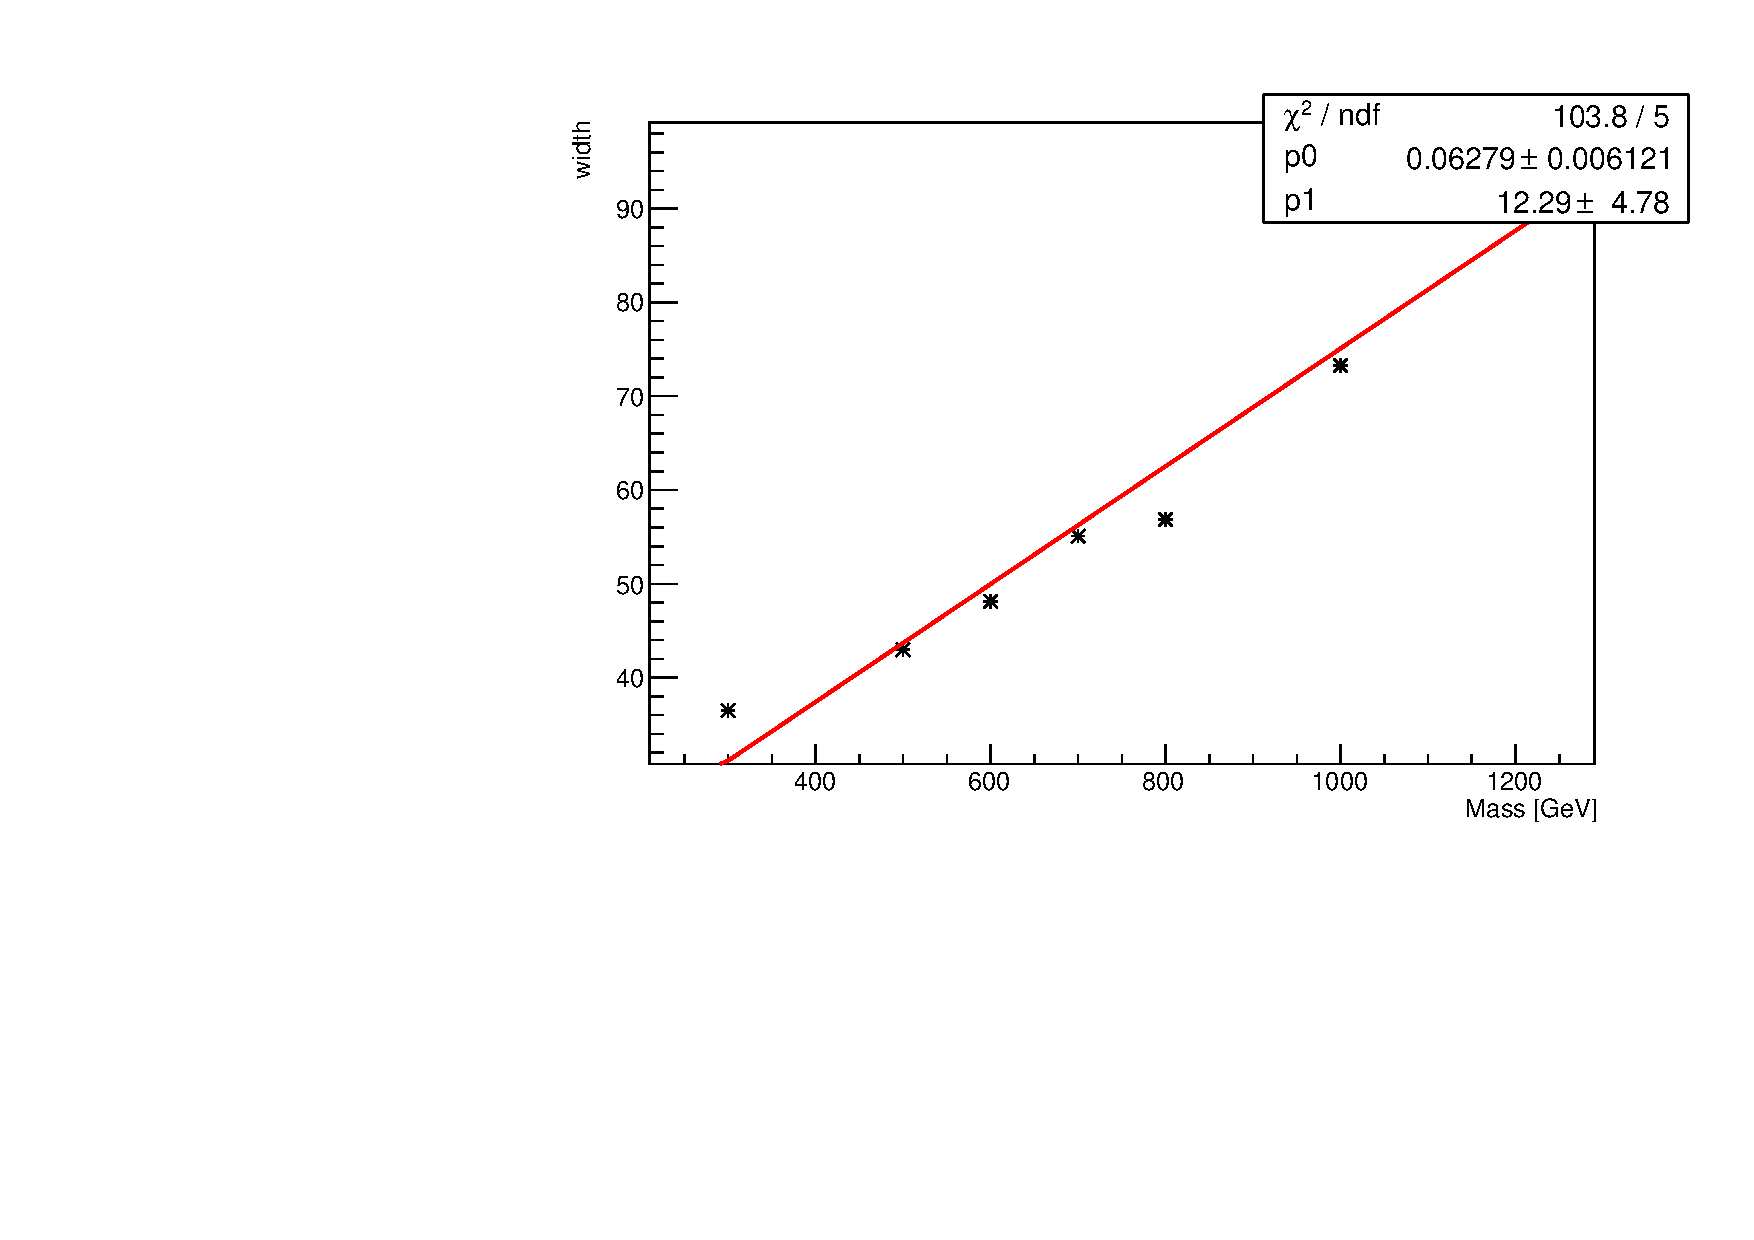
\includegraphics[width=0.48\hsize]{figures/Analysis/signal_mass_resolution/sigres_resolved_1lephvt.pdf}
    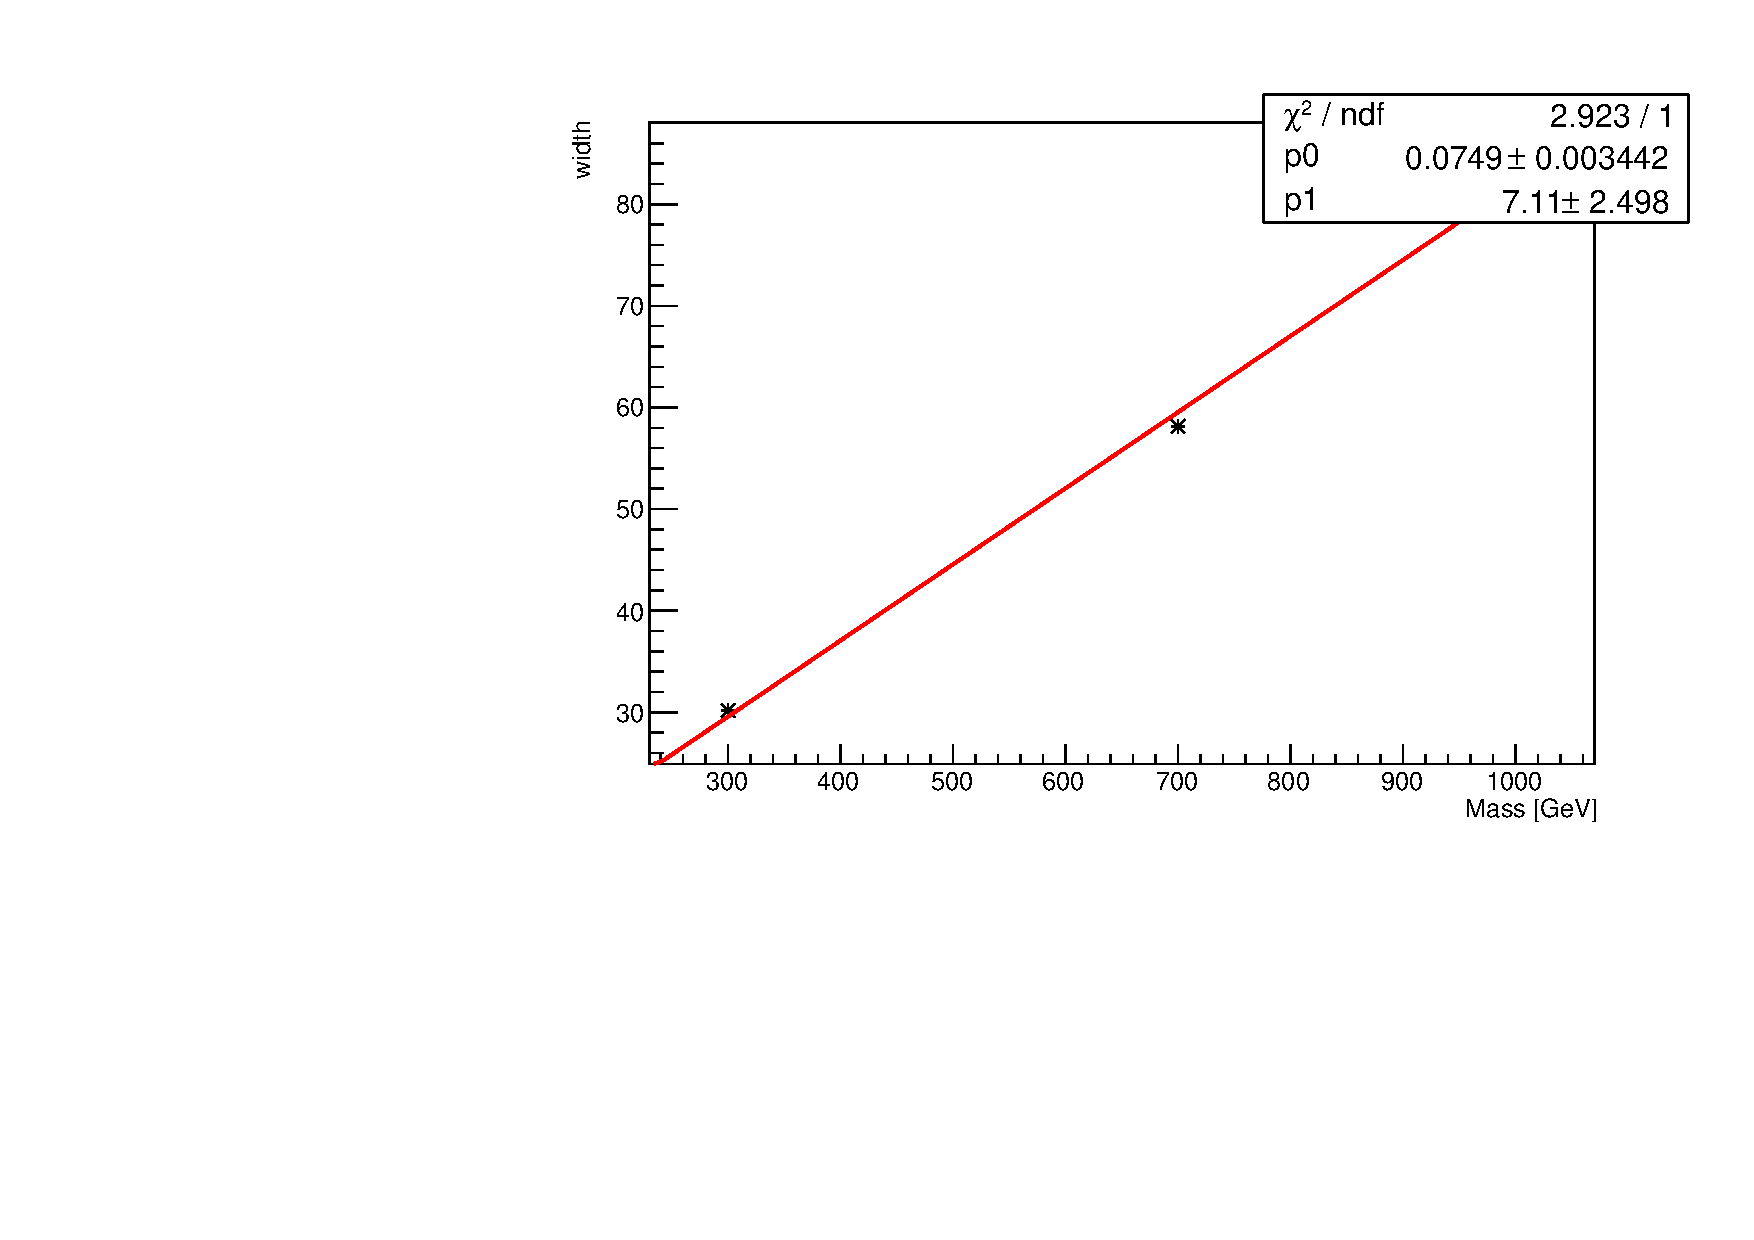
\includegraphics[width=0.48\hsize]{figures/Analysis/signal_mass_resolution/sigres_resolved_1lephvtvbf.pdf}
 \caption{The HVT signal mass resolution as a function of mass fit with a straight line in the Resolved ggF region (left) and VBF (right) region. } 
  \label{fig:resolved_sigwidth}
\end{figure} 
\FloatBarrier

\begin{figure}[h!]
  \centering
  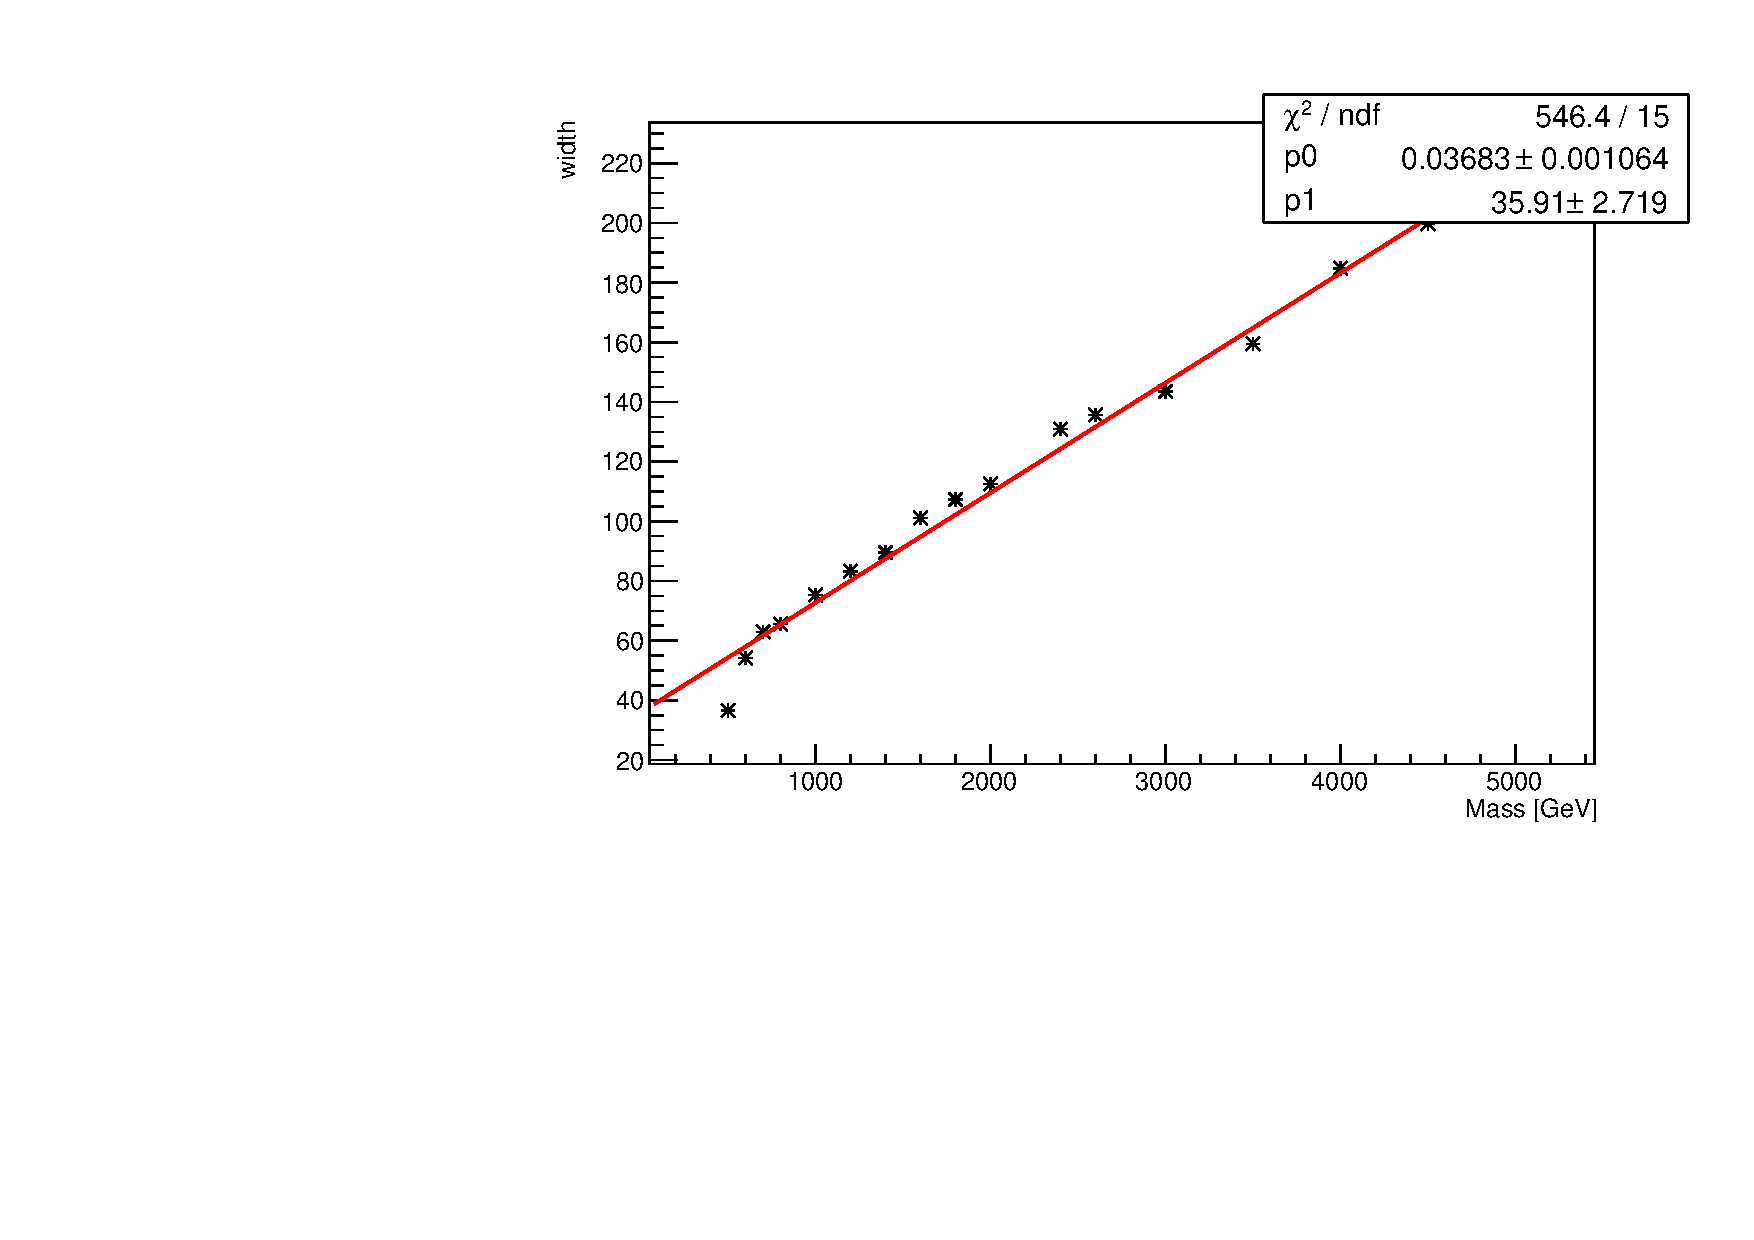
\includegraphics[width=0.48\hsize]{figures/Analysis/signal_mass_resolution/sigres_merged_1lephvt.pdf}
    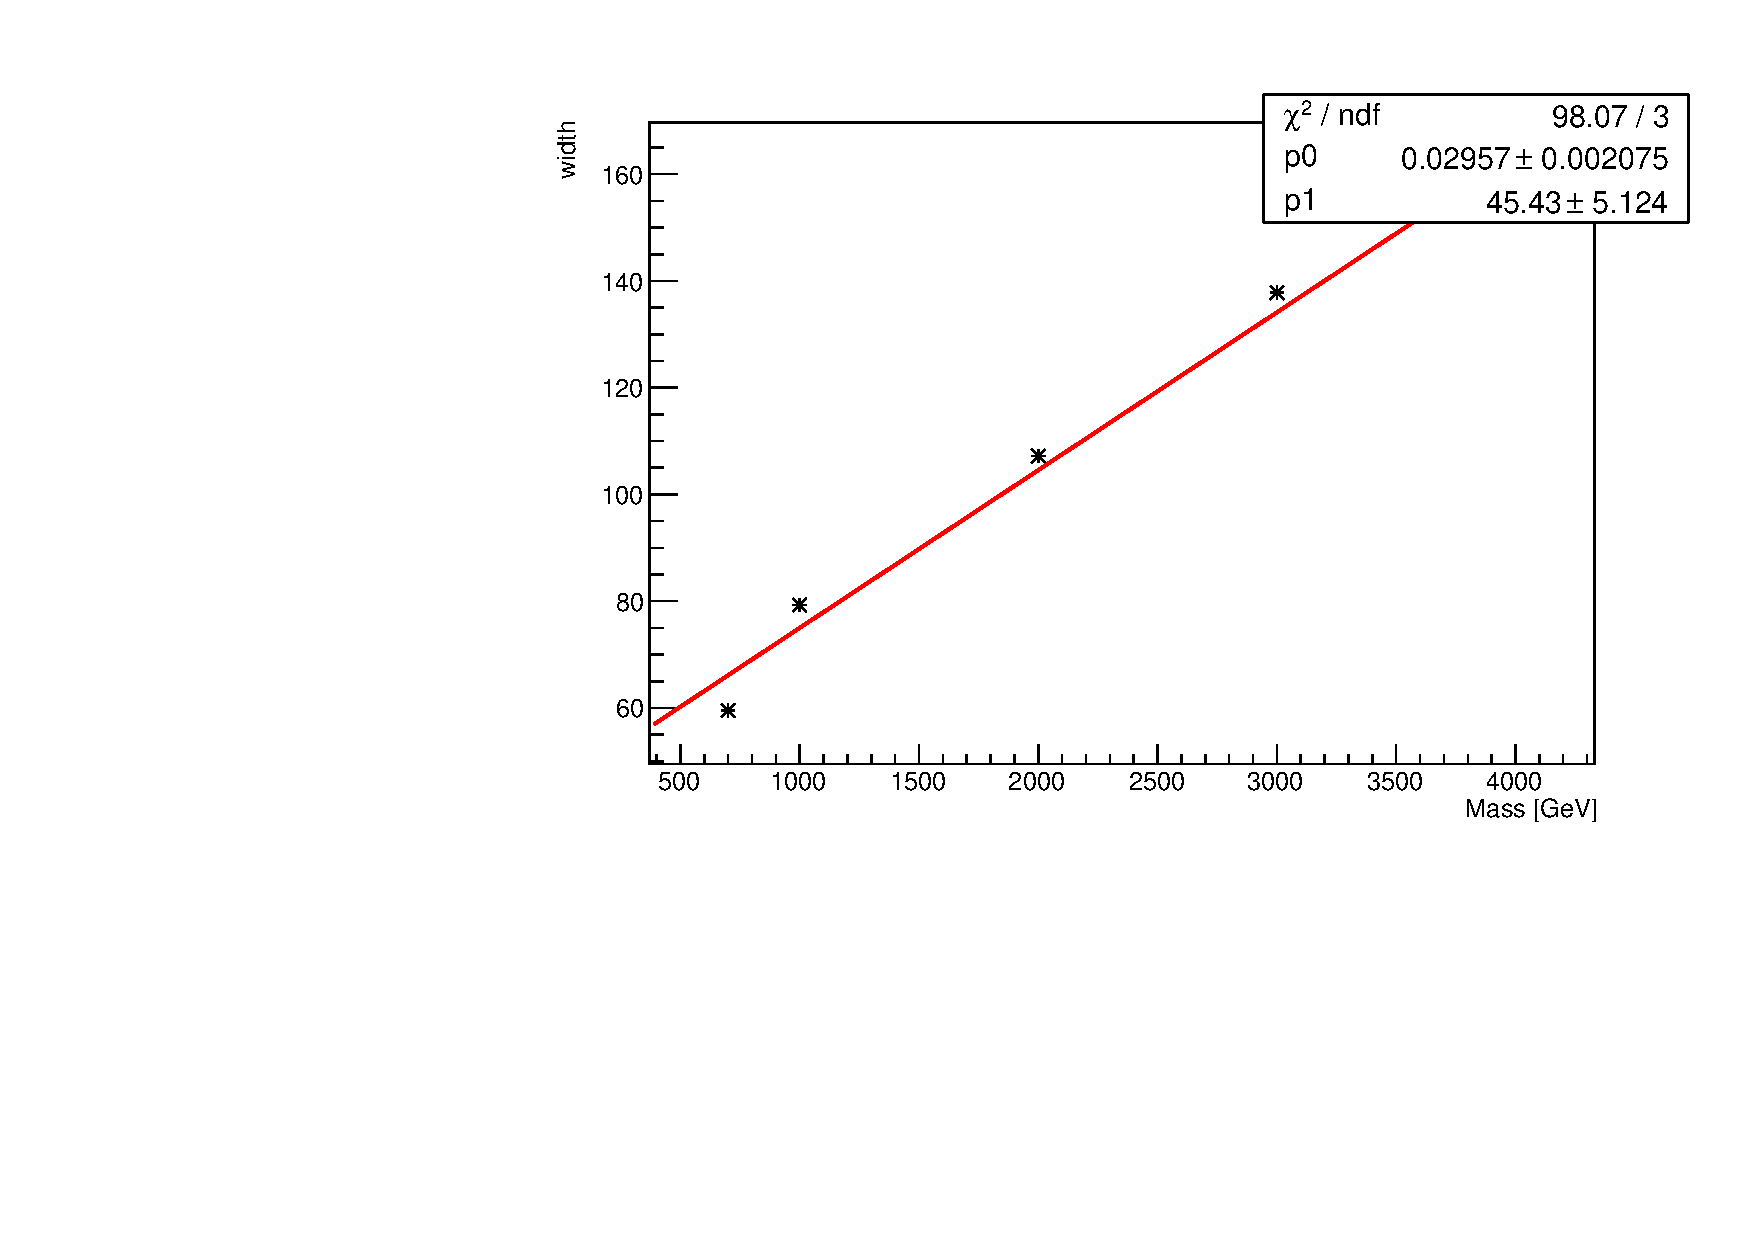
\includegraphics[width=0.48\hsize]{figures/Analysis/signal_mass_resolution/sigres_merged_1lephvtvbf.pdf}
 \caption{The HVT signal mass resolution as a function of mass fit with a straight line in the Merged ggF region (left) and VBF (right) region. } 
  \label{fig:merged_sigwidth}
\end{figure} 
\FloatBarrier

\section{Best Fit $\mu$}
The best fit signal strength parameter is denoted by $\hat{\mu}$ and calculated by maximizing the likelihood function with respect to all systematics and $\mu$. The corresponding set of systematics that maximize the likelihood are given by $\bm{\hat{\mu}}$. The first term in the likelihood is maximized when the expected number of signal and background events is equal to the number of events in data ($n_{ci}=\mu s_{ci} + b_{ci}$). Thus, by maximizing the likelihood, the fit determines values of $\mu$ and $\bm{\theta}$ that give the best agreement between expected and measured event yields. The second term in the likelihood is a penalty term which decreases the likelihood when systematics are shifted from their nominal values. This prevents the fit from profiling systematics in unphysical ways to maximize the likelihood. The uncertainty on $\mu$ is calculated by varying $\mu$ up and down until the natural log of the likelihood function shifts by one-half.


\section{Discovery Test}
To determine if the observed dataset is consistent with tested signal model a likelihood ratio is constructed:

\begin{equation}
\lambda(\mu)=\frac{\mathcal{L}(\mu, \hat{\hat{\bm{\theta_{\mu}}}})}{\mathcal{L}(\hat{\mu}, \hat{\bm{\theta}})}
\end{equation}

The denominator in this equation is the maximized value of $\mathcal{L}$ over all systematics and $\mu$. The numerator is the maximized likelihood over all systematics for a given $\mu$ value, where the maximized systematics are given by $\hat{\hat{\mu_{\mu}}}$. To test for the existence of signal the observed dataset the null hypothesis ($H_{0}$) is defined as the background only hypothesis and the alternate hypothesis includes signal and background ($H_{1}$). This test quantifies the compatibility of observed data with $H_{0}$ by calculating a p-value representing the probability of observing data as discrepant or more than the observed data under the $H_{0}$. The test statistic used to calculate this p-value is given by ($r_{0}$):

\begin{equation}
r_{0}=\left\{ \begin{array}{ll}
-2\ln \lambda (0), \hat{\mu} > 0\\
+2\ln \lambda (0), \hat{\mu} < 0
\end{array}
\right.
\end{equation}

The expected distribution of the the test statistic under $H_{0}$ ($f(r_{0}|0)$ is used to calculate the p-value:

\begin{equation}
p_{0}=\int_{r_0,obs}^{\infty} f(r_{0}|0)dr_{0}
\end{equation}

Small p-values indicate the observed data is poorly described by $H_{0}$. This equivalent Z-score of a given p-value is usually used to further quantify the agreement between the observed data and $H_{0}$. The Z-score is given by the number of standard deviations away from the mean of a Gaussian distribution, the integral of the upper tail of the distribution would equal the p-value. Mathematically:

\begin{equation}
Z = \Phi^{-1}(1-p_{0})
\end{equation}

where $\Phi$ is the Gaussian cumulative distribution function. The statistical significance of these tests are expressed as the $Z$-score. In particle physics, $3\sigma$ is considered evidence for new phenomena and $5\sigma$ is the threshold for discovery. 
\section{Exclusion Limits}
In the absence of discovery, upper limits on the signal strength, $\mu$ are set using the CLs method [cite P60]. The test statistic for this test, $q_{\mu}$, is constructed as:
\begin{equation}
\tilde{\lambda_{\mu}}=\left\{ \begin{array}{ll}
\frac{\mathcal{L}(\mu,\hat{\hat{\theta_{\mu}}})}{\mathcal{L}(\hat{\mu},\hat{\theta})},  \hat{\mu} > 0\\
\frac{\mathcal{L}(\mu,\hat{\hat{\theta_{\mu}}})}{\mathcal{L}(0,\hat{\hat{\theta_{0}}})},  \hat{\mu} < 0
\end{array} 
\right.
\end{equation}
 
 \begin{equation}
\tilde{q}_{\mu}=\left\{ \begin{array}{ll}
-2\ln \tilde{\lambda}(\mu),  \hat{\mu} < \mu \\
+2\ln \tilde{\lambda}(\mu),  \hat{\mu} > \mu 
\end{array}
\right.
\end{equation}
 
As defined, larger values of $q_{\mu}$ correspond to increasing incompatibility between the observed data and the background + signal hypothesis. The observed value of the test statistic, $q_{\mu, obs}$, is then compared to its expected distribution, $f$, to calculate p-values to assess the likelihood of the background+signal hypothesis. Using these distributions, $CL_{s}$ values are computed as:
 
 \begin{equation}
 CL_{s+b}=\int_{q_{\mu, obs}}^{\infty}f(q_{\mu}|\mu)dq_{\mu}\\
 \end{equation}
  \begin{equation}
CL_{b}=\int_{q_{0}^{obs}}^{\infty}f(q_{\mu}|\mu=0)dq_{\mu}\\
 \end{equation}
  \begin{equation}
CL_{s}=\frac{CL_{s+b}}{CL_{b}}
 \end{equation}

$CL_{s+b}$ is the p-value for the signal + background hypothesis and $CL_{b}$ is the p-value for the background only hypothesis. The $CL_{s}$ value is interpreted as the probability to observe the background + signal hypothesis normalized to the probability of background-only hypothesis. Normalizing by $CL_{b}$ prevents setting artificially strong exclusion limits due to downward fluctuations in data. 

For a given signal hypothesis, $\mu$ values are scanned simultaneously over all $m_{WV}$ bins to find the $\mu$ value that yields $CL_{s}$=0.05, meaning the likelihood of finding data more incompatible with the signal+background hypothesis (relative to the background only hypothesis) is 5\%. The 95\% upper limit on the cross section is then calculated as the product of the $\mu$ value found, branching ratio, and theory cross section.







